\documentclass[a4paper,
fontsize=11pt,
%headings=small,
oneside,
numbers=noperiodatend,
parskip=half-,
bibliography=totoc,
final
]{scrartcl}

\usepackage[babel]{csquotes}
\usepackage{synttree}
\usepackage{graphicx}
\setkeys{Gin}{width=.8\textwidth} %default pics size

\graphicspath{{./plots/}}
\usepackage[ngerman]{babel}
\usepackage[T1]{fontenc}
%\usepackage{amsmath}
\usepackage[utf8x]{inputenc}
\usepackage [hyphens]{url}
\usepackage{booktabs} 
\usepackage[left=2.4cm,right=2.4cm,top=2.3cm,bottom=2cm,includeheadfoot]{geometry}
\usepackage[labelformat=empty]{caption} % option 'labelformat=empty]' to surpress adding "Abbildung 1:" or "Figure 1" before each caption / use parameter '\captionsetup{labelformat=empty}' instead to change this for just one caption
\usepackage{eurosym}
\usepackage{multirow}
\usepackage[ngerman]{varioref}
\setcapindent{1em}
\renewcommand{\labelitemi}{--}
\usepackage{paralist}
\usepackage{pdfpages}
\usepackage{lscape}
\usepackage{float}
\usepackage{acronym}
\usepackage{eurosym}
\usepackage{longtable,lscape}
\usepackage{mathpazo}
\usepackage[normalem]{ulem} %emphasize weiterhin kursiv
\usepackage[flushmargin,ragged]{footmisc} % left align footnote
\usepackage{ccicons} 
\setcapindent{0pt} % no indentation in captions

%%%% fancy LIBREAS URL color 
\usepackage{xcolor}
\definecolor{libreas}{RGB}{112,0,0}

\usepackage{listings}

\urlstyle{same}  % don't use monospace font for urls

\usepackage[fleqn]{amsmath}

%adjust fontsize for part

\usepackage{sectsty}
\partfont{\large}

%Das BibTeX-Zeichen mit \BibTeX setzen:
\def\symbol#1{\char #1\relax}
\def\bsl{{\tt\symbol{'134}}}
\def\BibTeX{{\rm B\kern-.05em{\sc i\kern-.025em b}\kern-.08em
    T\kern-.1667em\lower.7ex\hbox{E}\kern-.125emX}}

\usepackage{fancyhdr}
\fancyhf{}
\pagestyle{fancyplain}
\fancyhead[R]{\thepage}

% make sure bookmarks are created eventough sections are not numbered!
% uncommend if sections are numbered (bookmarks created by default)
\makeatletter
\renewcommand\@seccntformat[1]{}
\makeatother

% typo setup
\clubpenalty = 10000
\widowpenalty = 10000
\displaywidowpenalty = 10000

\usepackage{hyperxmp}
\usepackage[colorlinks, linkcolor=black,citecolor=black, urlcolor=libreas,
breaklinks= true,bookmarks=true,bookmarksopen=true]{hyperref}
\usepackage{breakurl}

%meta
%meta

\fancyhead[L]{K. Schuldt\\ %author
LIBREAS. Library Ideas, 44 (2023). % journal, issue, volume.
%\href{https://doi.org/10.18452/27071}{\color{black}https://doi.org/10.18452/27071}
{}} % doi 
\fancyhead[R]{\thepage} %page number
\fancyfoot[L] {\ccLogo \ccAttribution\ \href{https://creativecommons.org/licenses/by/4.0/}{\color{black}Creative Commons BY 4.0}}  %licence
\fancyfoot[R] {ISSN: 1860-7950}

\title{\LARGE{Völkisches Büchereiwesen} \vskip 1em \large{Zur Geschichte der Grenzbüchereiarbeit in der Weimarer Republik und im Nationalsozialismus}}% title
\author{Karsten Schuldt} % author

\setcounter{page}{1}

\hypersetup{%
      pdftitle={Völkisches Büchereiwesen. Zur Geschichte der Grenzbüchereiarbeit in der Weimarer Republik und im Nationalsozialismus},
     pdfauthor={Karsten Schuldt},
      pdfcopyright={CC BY 4.0 International},
      pdfsubject={LIBREAS. Library Ideas, 44 (2023).},
      pdfkeywords={Öffentliche Bibliotheken, Büchereiwesen, Fachstellen, Bibliotheksgeschichte, völkisches Denken, Weimarer Republik, Nationalsozialismus, Büchereipädagogik, Public libraries, Public librarianship, Fachstellen, library history, völkisch ideology, Weimar republic, Nationalsocialism, Büchereipädagogik},
      pdflicenseurl={https://creativecommons.org/licenses/by/4.0/},
      pdfurl={https://doi.org/},
      pdfdoi={10.18452/},
      pdflang={de},
      pdfmetalang={de}
     }



\date{}
\begin{document}

\maketitle
\thispagestyle{fancyplain} 

%abstracts
\begin{abstract}
\noindent
Das Öffentliche Bibliothekswesen -- vor den 1970er Jahren eher
Büchereiwesen genannt -- ist immer eingelassen in die zeitgenössischen
Denkweisen und politischen Entwicklungen der Gesellschaft, im den es
existiert. Gleichzeitig findet die Weiterentwicklung der Büchereiarbeit
sowie der Infrastrukturen des Büchereiwesens statt, egal welche
Ideologie jeweils aktuell vorherrschend sind. Der Artikel zeigt dies am
Beispiel des Grenzbücherdienst e.V. auf, welcher in den 1920er bis
1940er Jahren in Deutschland eine bedeutende Rolle im damaligen
Bibliothekswesen spielte, obwohl die Grundüberzeugungen, die der Verein
vertrat, heute als rechtsextrem gelten können. Der Verein ging von einem
völkischen Verständnis aus, nach dem die Welt in Völker eingeteilt wäre,
die sich untereinander bekämpfen würden und sah es als seine Aufgabe
darin, die «Erhaltung» des deutschen Volkes in den sogenannten
«Grenzregionen» sicherzustellen. Für seine Arbeit konnte der Verein
offenbar enorme Ressourcen mobilisieren. Er war mit den entstehenden
staatlichen Infrastrukturen des Büchereiwesens, insbesondere den damals
gegründeten Fachstellen, verbunden und war zudem eingelassen in die
zeitgenössischen Diskurse des Büchereiwesens, insbesondere der
Büchereipädagogik. Er nutzte nicht nur die gleichen Instrumente, wie sie
auch von deutschen Büchereien genutzt wurden, die der Verein nicht
erreichte. Vielmehr trieben einige Mitglieder des Vereins in ihren
beruflichen Funktionen, beispielsweise als Fachstellenleitungen, die
Entwicklung des Bücherwesens selber mit voran. Der Text schildert, nach
einer notwendigen historischen Kontextualisierung, die vom Verein
verbreiteten Diskurse und seine konkrete Arbeit, zuerst während der
Weimarer Republik (1918-1933), dann während des Nationalsozialismus
(1933-1945). Dabei wird sich zeigen, dass die Ideologie und konkrete
Tätigkeit des Vereins ohne grössere Probleme auch in das
nationalsozialistische Büchereiwesen integriert werden konnte. Am Ende
stellt sich die Frage, was aus dieser Geschichte über das heutige
Öffentliche Bibliothekswesen gelernt werden kann.

\begin{center}\rule{0.5\linewidth}{0.5pt}\end{center}

Public libraries -- before the 1970s called «Büchereien» in german -- is
always connected to the contemporary discourses and political
developments of the society there in. Regardless of the dominant
ideologies, the advancements of the libraries work as well as the
infrastructures of librarianship continues. This article shows this by
example of the Grenzbüchereidienst e.V., which played an important role
in german public librarianship during the 1920s to 1940s, although the
basic beliefs of this association are seen as extreme right-wing
ideologies today. The association followed a ``völkische''
understanding, by which the world is divided into ``Völker'' (ethnic
groups) which are in a constant struggle between each other. He saw his
goal in the upkeep of the german ``Volk'' in the so called
``Grenzregionen'' (border regions). For their work the association was
apparently able to mobilise a great deal of ressources. He was conceted
to the infrastructures of libarrianship, which where developing at that
time, especially to the new founded ``Fachstellen'' (central departemts
for the support of public libraries) and accepted the contemporary
discourses of german public librarianship, expressly the
``Büchereipädagogik'' (a form of planed education through public
libraries, unique for libraries in the german speaking countries). The
association used the same instruments and methods like those public
libraries which she did not reach. In fact, members of the association
pushed the development of public librarianship at that time
themselves,in their professional roles, e.g.~as directors of the
aforementioned ``Fachstellen''. After a necessary historical
contextualisation, this article depicts the discourses as well as the
concret activities of the association during the Weimar republic
(1918-1933) and the nationalsocialist regime (1933-1945). Thereby it
will become clear apparent, that the basic belives as well as the work
of the association could easily be integrated into the public
librarianship during the nazi area. At the end, the article raises
questions, what could be learned from this history for todays public
librarianship.
\end{abstract}

%body
Inhaltswarnung: Dieser Text beschäftigt sich mit völkisch denkenden
Personen während der Weimarer Republik und dem Nationalsozialismus. Er
enthält Originalzitate, welche völkische, explizit rassistische sowie
antisemitische Begrifflichkeiten nutzen, um ebensolche Inhalte
darzustellen.

\begin{quote}
«Im Leben eines Volkes liegen Wirtschaft, Politik und Kultur so
ineinander und durcheinander geschichtet, daß man sie nicht säuberlich
voneinander trennen kann und daß man nicht behaupten kann, das eine oder
andere Organ sei das Wichtigste. Zuletzt wird immer dasjenige Volk sich
politisch und wirtschaftlich behaupten, daß seine geistigen und
seelischen Kräfte voll entwickelt. Eine solche volle harmonische
Entwicklung muß man besonders einer Grenzbevölkerung wünschen, die ja
infolge ihrer Randlage schon sowieso in dem Nachteil lebt, daß in ihr
die geistigen Lebensströme der Nation schwächer pulsieren. Gerade in
einer Zeit, da die wirtschaftlichen Kräfte in den Grenzgebieten so
geschwächt sind, muß mit erhöhtem Nachdruck die Forderung gestellt
werden, daß die bedrohte völkische Lebenskraft von der kulturellen Seite
her so pfleglich wie möglich behandelt wird. {[}\ldots{]}

Die Aufgabe also, hierfür das deutsche Buch als den Rückhalt und Träger
deutscher Kultur planmäßig einzusetzen, kann in dieser Stunde nicht
ernst genug genommen und gelöst werden. Gibt es doch kein Gebiet des
Lebens, in das es nicht befruchtend oder auch zerstörerisch hineinwirkt.
Es kann sich also bei der Pflege des Buches in den Grenzgebieten immer
nur um einen kulturell und pädagogisch geregelten Einsatz handeln, wozu
öffentliche, kräftig entwickelte Büchereien notwendig sind.» (Schriewer
1933a: 7f.)
\end{quote}

\hypertarget{einleitung}{%
\section{1. Einleitung}\label{einleitung}}

Gegenstand dieses Artikels sind die zu damaliger Zeit
«Grenzbüchereiarbeit» genannten Tätigkeiten, welchen in Deutschland
während der Weimarer Republik (1918--1933) und dem Nationalsozialismus
(1933--1945) nachgegangen wurde. Bei dieser Arbeit ging es immer um die
damals zumeist «Volksbüchereien» genannten Vorläufer der heutigen
Öffentlichen Bibliotheken, wobei dazu oft auch Bibliotheken gezählt
wurden, die heute «Schulbibliotheken» heissen würden. Es wird
thematisiert, wie die Entwicklung von Strukturen des deutschen (und,
spätestens durch die 1938 erfolgte Angliederung an das Deutsche Reich,
österreichischen) Volksbüchereiwesens explizit verbunden waren mit einer
Ideologie, die heute zurecht als explizit rechtsextrem gilt.

\hypertarget{struktur-des-zeitgenuxf6ssischen-volksbuxfcchereiwesens}{%
\subsection{1.1 Struktur des zeitgenössischen
Volksbüchereiwesens}\label{struktur-des-zeitgenuxf6ssischen-volksbuxfcchereiwesens}}

Die sich zu heute unterscheidenden Bezeichnungen sind sichtbarer
Ausdruck einer damals auch anders als heute strukturierten
Büchereilandschaft, welche bei der Geschichte der Grenzbüchereiarbeit
beachtet werden muss.

Während die Öffentlichen Bibliotheken heute, ungeachtet der
verschiedenen Träger (Gemeinden, Gemeindeverbände, Stiftungen, Vereine,
Kirchgemeinden, nicht profitorientiert arbeitende Firmen und so weiter),
Teil der von Gemeinden beziehungsweise Städten finanzierten und
beauftragten Infrastruktur von Bildungs- und Kultureinrichtungen sind,
galt dies in der hier untersuchten Zeit nicht. Vielmehr ist die
Grenzbüchereiarbeit Teil der Geschichte der «Kommunalisierung» des
Öffentlichen Büchereiwesens, also der langsamen «Erhöhung der
Staatsquote» in diesem Bereich. Zu Beginn des 20. Jahrhunderts waren
Volksbüchereien in Deutschland und Österreich (die beiden Länder, welche
in diesem Artikel die Hauptrolle spielen werden) institutionell nicht
eindeutig verankert: Zum Teil wurden sie von Vereinen betrieben, zum
Teil von Gemeinden und oft auch von Lehrern an den damals zumeist
Volksschulen genannten Einrichtungen (die heute Grund- oder Primarschule
heissen und selbstverständlich, im Vergleich zum Zeitraum von
1918--1945, zum Teil auch andere Aufgaben haben). Es war auch nicht
ungewöhnlich, wenn in grossen Betrieben sogenannte Werkbüchereien als
Teil der Sozialeinrichtungen für die Belegschaft betrieben wurden, die
zum Büchereiwesen der damaligen Zeit zu zählen sind. Darüber hinaus gab
es zahlreiche, an politische Bewegungen und Milieus angebundene
Büchereien, insbesondere die explizit von katholischen Vereinen und
Kirchgemeinden betriebenen («katholische Bibliotheken») sowie solche von
sozialdemokratischer beziehungsweise gewerkschaftlicher Seite
(«Arbeiterbibliotheken»). Genaue Zahlen über die Anzahl, Grösse und
Verbreitung all dieser Büchereien sind heute nicht mehr verfügbar. Aber
es wäre falsch, die von den Gemeinden direkt geführten und finanzierten
Büchereien als die grössten oder erfolgreichsten anzusehen und die
anderen nur als kleine Einrichtungen. Oft scheint das Gegenteil der Fall
gewesen zu sein.\footnote{Vergleiche Wild (1957), damals Leiterin der
  Öffentlichen Bibliotheken der Stadt Zürich, die noch Ende der 1950er
  Jahre darüber schreibt, dass die beiden Arbeiterbibliotheken der Stadt
  weit höhere Ausleihzahlen hätten als die von ihr geleiteten.} Nicht
zuletzt gab es zahllose gewerblich organisierte «Leihbibliotheken».

Zudem kamen zu den Büchereien -- in denen Bücher ausgeliehen wurden --
Lesehallen. In diesen wurden Bücher, später auch Zeitschriften und
Zeitungen, zum Lesen vor Ort vorgehalten. Büchereien und Lesehallen
konnten getrennt voneinander existieren, aber auch in einer Einrichtung
zusammengeführt sein. Teilweise wurden sie zusammen betrieben, teilweise
gab es auch am selben Ort zum Beispiel Vereine, die Büchereien und
solche, die Lesehallen unterhielten. Zudem waren die Grenzen nicht immer
klar gezogen -- nur, weil eine Einrichtung Lesehalle hiess, bedeutete
das nicht unbedingt, dass sie nicht auch Bücher entlieh. Und, um die
Sache noch komplizierter zu machen, gab es beispielsweise ab ungefähr
1910 auch explizite «Kinderlesehallen» (Feldhausen 1910), teilweise als
eigenständige Einrichtungen oder als Filialen von Volksbüchereien,
teilweise als eigene Räume innerhalb einer Volksbücherei. Welche
Aufgaben die Büchereien und Lesehallen hatten, war die ganze Zeit über
nicht genau geklärt, vielmehr war es Thema intensiver
Auseinandersetzungen. Erst die «Kommunalisierung» führte dazu, dass sich
ein gewisses, gemeinsam geteiltes Verständnis dieser Aufgaben
entwickelte. Dieser Prozess zog sich bis in die 1960er Jahre des 20.
Jahrhunderts, war also am Ende des hier besprochenen Zeitraumes nicht
abgeschlossen.

In der Grenzbüchereiarbeit ging es aber immer um Volksbüchereien,
inklusive derer in Schulen, und in der späten Weimarer Republik auch
manchmal um die katholischen Bibliotheken. Arbeiterbibliotheken und
Leihbibliotheken wurden immer als «gegnerische» Einrichtungen angesehen,
auch die katholischen Bibliotheken wurden nach 1933 wieder abgelehnt.

\hypertarget{fokus-und-ziele-des-artikels}{%
\subsection{1.2 Fokus und Ziele des
Artikels}\label{fokus-und-ziele-des-artikels}}

Dieser Artikel beschränkt sich, wie schon gesagt, auf Deutschland und --
bedingt durch den 1938 erfolgten «Anschluss» an das Deutsche Reich --
auf Österreich. Dies hat einerseits mit den hier verwendeten Quellen zu
tun, andererseits ist -- wie im nächsten Kapitel noch einmal besprochen
wird -- das «völkische Denken» zumindest in dieser Intensität eine
Spezifik der deutschen und österreichischen Gesellschaften Ende des 19.
und Anfang des 20. Jahrhunderts. Ob, und wenn ja wie, ein ähnliches
Denken auch die Entwicklung der Volksbüchereien in anderen Ländern
beeinflusst hat, muss eine Frage für weitere Forschungen bleiben.

Ziel dieses Textes hier ist -- auch das wird weiter unten nochmal
thematisiert -- explizit nicht, eine Verurteilung des damaligen
Büchereiwesens vorzunehmen, Einzelpersonen aus dem damaligen
Bibliothekswesen zu diskreditieren oder die damals aufgebauten und heute
noch existierenden bibliothekarischen Infrastrukturen zu verurteilen. Es
sollte aus der unten folgenden Darstellung ersichtlich werden, dass die
gesamte völkische Ideologie und damit auch die daraus abgeleiteten
«Probleme», Lösungen und so weiter, inhaltlich und moralisch falsch
waren und zu verurteilen sind. Es ist aber nicht vorrangiges Ziel dieses
Artikels, dies explizit nachzuweisen. Vielmehr geht es hier darum, zu
zeigen, wie eng die Entwicklung von Bibliotheken und die Entwicklungen
der jeweiligen Gesellschaft zusammenhängen. Wenn der Text eines zeigen
soll, dann, dass Vorstellungen davon, dass Öffentliche Bibliotheken oder
ihre Vorgänger immer schon bestimmte Werte vertreten oder gelebt hätten
(beispielsweise einen «demokratischen Kern» hätten), die frei von den
gesellschaftlichen Entwicklungen wären, falsch sind.

In diesem Text wird ein Autor, Franz Schriewer, sehr oft angeführt
werden. (Schon das eröffnende Zitat stammt von ihm.) Schriewer ist heute
wohl vor allem bekannt dafür, das Öffentliche Bibliothekswesen in
Schleswig-Holstein aufgebaut sowie gleichzeitig mittels seiner
Vereinsarbeit und Artikel das Bibliothekswesen der frühen Bundesrepublik
Deutschland geprägt zu haben. Deswegen kann leicht der Eindruck
entstehen, als würde es in diesem Text darum gehen, nachträglich zu
zeigen, dass Schriewer zuvor unter dem Nationalsozialismus eine -- wenn
auch nicht ganz ungebrochene -- Karriere hatte. Angesichts dessen, dass
die Kontinuitäten bibliothekarischer Karrieren in Deutschland vor und
nach 1945 erst seit den 1970er Jahren wirklich thematisiert werden
(Andrae 1970, Kettel 1981, Boese 1987) wäre dies denkbar. Aber: Erstens
müsste man die Geschichte hier erweitern. Schriewer war schon in der
Weimarer Republik ein erfolgreicher Organisator der Büchereiarbeit in
Schleswig -- bei ihm explizit als «Grenzbüchereidienst» verstanden --
und nicht erst nach 1933. Zweitens wird Schriewer in diesem Artikel hier
vor allem deshalb oft zitiert, weil er einfach die gesamte Zeit über ein
überaus produktiver Autor war. (Vergleiche seine Bibliographie in Weimar
1976.) Er publizierte kontinuierlich praktisch sofort seit er 1921 mit
dem Bibliotheksdienst begann und bis nach seiner Verrentung 1959. In
fast allen zeitgenössischen wichtigen bibliothekarischen Zeitschriften
fanden sich von ihm regelmässig Artikel, Rezensionen und Kommentare. Die
inhaltliche Breite seiner Arbeiten ist beachtlich: Von
büchereitechnischen Entwicklungen (Schriewer 1924b) über
büchereipolitische Grundsatzartikel (Schriewer 1933b) bis hin zu
zahllosen Besprechungen. (Schriewer 1933c) Zudem hielt er ständig
Vorträge und leitete Weiterbildungsveranstaltungen, die von anderen
Autor*innen referiert wurden. (Scheffen-Döring 1933) Er hat seine
Karriere und inhaltliche Entwicklung praktisch selber gut dokumentiert.
Schon die jeweiligen Zusätze zu seinem Autorennamen («Flensburg»,
«Berlin», «Frankfurt/Oder») berichten von seinen Karrierewegen.
Ungezählte andere Bibliothekar*innen machten zur gleichen Zeit ähnliche,
aber eben nicht mehr so einfach nachvollziehbare, Karrieren im deutschen
Büchereiwesen, über alle politischen Veränderungen hinweg.\footnote{Wenn
  man einen anderen deutschen Bibliothekar mit vergleichbarer
  «Sichtbarkeit» und Karriere in verschiedenen deutschen Staaten sucht,
  müsste man wohl auf Heinrich Uhlendahl verweisen, der in der Weimarer
  Republik Direktor der Deutschen Bibliothek in Leipzig wurde, das die
  ganze Zeit des Nationalsozialismus über blieb, die Bibliothek die
  gesamte Zeit der US-amerikanischen und sowjetischen Besatzung von
  Leipzig bis weit über die Gründung der DDR hinaus leitete -- und dann,
  mit hohen Ehren verabschiedet, in den Ruhestand ging. (Flachowsky
  2018, Rau 2018)} Nicht zuletzt wurde, drittens, von Uwe Danker schon
ein Beitrag zur Biographie Schriewers, inklusive einer kritischen
Wertung seines Verhaltens während des Nationalsozialismus, vorgelegt.
(Danker 2017) Wenn es darum gehen würde, direkt an diesen Beitrag
anzuschliessen, müsste hier, im vorliegenden Artikel, ein neuer Fokus
gewählt werden. Aber es geht hier gerade nicht darum, Schriewer hier als
besonders zu zeichnen. Wenn überhaupt, dann steht er als einer von
vielen im deutschen Bibliothekswesen. (Vergleiche auch den gesamten Band
Kuttner \& Vodosek 2017, nicht nur den Beitrag von Danker.)

Wichtig ist an dieser Stelle zudem, explizit darauf hinzuweisen, dass es
sich beim hier im Mittelpunkt stehenden \emph{Grenzbüchereidienst e.V.}
nicht um eine randständige Organisation handelte, die vielleicht keinen
Einfluss auf das Büchereiwesen hatte. Vielmehr waren die Aktiven des
Vereins eng mit dem restlichen Büchereiwesen -- zumindest der Richtung
der «Volksbüchereien», nicht der anderen drei weiter oben genannten
«Richtungen» katholische Bibliotheken, Arbeiterbibliotheken und
gewerbliche Leihbibliotheken -- verbunden. Ein grosser Teil von ihnen
publizierte regelmässig auch in den jeweiligen Zeitschriften für das
Volksbüchereiwesen (also vor allem den \emph{Blättern für
Volksbüchereien und Lesehallen} (1900--1919), der \emph{Bücherei und
Bildungspflege} (1920--1933) und \emph{Die Bücherei} (1933--1944), aber
auch vielen kleineren Blättern\footnote{In den \emph{Heften für
  Büchereiwesen} (unregelmässig 1920--1932), der damals zweiten
  reichsweit erscheinenden Fachzeitschrift für Volksbüchereien, wurde
  der Verein und das Thema nicht erwähnt.}), war in den
bibliothekarischen Verbänden, auf den Kongressen und den
Weiterbildungsveranstaltungen vertreten und besetzte auch viele der
zentralen Stellen, die für die Entwicklung des Öffentlichen
Büchereiwesens, insbesondere ausserhalb der grossen Städte, wichtig
waren. Über die Aktivitäten des Vereins und die Themen, die er
bearbeitete, wurde in der restlichen bibliothekarischen Presse zudem oft
berichtet. (Vergleiche zum Beispiel Kander 1928) Nicht zuletzt war der
Verein gut mit den wirtschaftlichen Eliten Deutschlands verbunden.

\hypertarget{struktur-des-artikels}{%
\subsection{1.3 Struktur des Artikels}\label{struktur-des-artikels}}

Diesem einleitenden Kapitel folgt nun eines (2.), in dem Grundbegriffe
und Konzepte, welche für die Geschichte der Grenzbüchereiarbeit relevant
sind, geklärt werden. Insbesondere wird das völkische Denken sowie die
dominanten Vorstellungen zur Büchereipädagogik besprochen. Am Ende
dieses Kapitels wird auf das Anfangszitat dieses Textes zurückverwiesen,
um es im Kontext dieser Vorstellungen noch einmal zu lesen. Es wird sich
zeigen, dass es problematischer ist, als es auf den ersten Blick
erscheint und nicht nur einfach eine vielleicht etwas überkommene
Sprache verwendet. Anschliessend wird die Geschichte der
Grenzbüchereiarbeit während der Weimarer Republik dargestellt. (3.) In
der deutschen Geschichte wird im Allgemeinen das Jahr 1933 mit der
Machtergreifung der Nationalsozialisten als Bruchpunkt gesehen. Dem
folgt auch dieser Text, indem er die Geschichte der Grenzbüchereiarbeit
während dieses Herrschaftssystems in einem gesonderten Kapitel
darstellt. (4.) Allerdings kann hier schon gesagt werden, dass sich die
Grenzbüchereiarbeit in dieser Zeit eher kontinuierlich
weiterentwickelte. Einen echten Bruch gab es nicht. Im vorletzten
Kapitel (5.) wird dann die Grenzbüchereiarbeit aus der heutigen Sicht
bewertet. Grundsätzlich, um auch das vorwegzugreifen, endet die von
völkischem Denken geprägte Volksbüchereiarbeit mit dem Ende des
Nationalsozialismus. Aber viele Strukturen und Vorstellungen werden nach
1945 weitergeführt. Sie transformierten sich und nehmen heute auch
andere Aufgaben wahr -- die \emph{Büchereizentrale Schleswig-Holstein}
ist heute zum Beispiel eine ganz andere Einrichtung als Franz Schriewers
\emph{Zentrale für Nordmarkbüchereien} und hat auch ganz andere Ziele,
obgleich sie in einer direkten Kontinuität steht. Insoweit drängt sich
nicht nur die Frage auf, wie erfolgreich die Grenzbüchereiarbeit an sich
war, sondern auch, was diese Kontinuitäten für das heutige
Bibliothekswesen bedeuten -- oder nicht bedeuten.

\hypertarget{grundkonzepte}{%
\section{2. Grundkonzepte}\label{grundkonzepte}}

Zur Kontextualisierung der Grenzbüchereiarbeit ist es notwendig, im
Vorfeld zwei Themenkomplexe, nämlich völkisches Denken und
Büchereipädagogik, zu klären. Dies geschieht in den folgenden beiden
Abschnitten.

\hypertarget{vuxf6lkisches-denken}{%
\subsection{2.1 Völkisches Denken}\label{vuxf6lkisches-denken}}

Völkisches Denken, auf dem die «völkische Bewegung» in Deutschland und
Österreich Ende des 19. und Anfang des 20. Jahrhunderts aufbaute, hat
einen spezifischen Inhalt, auch wenn dieses Denken von Widersprüchen
gekennzeichnet war und deshalb nicht immer leicht zu fassen ist.
(Puschner, Schmitz \& Ulbricht 1996a, Hartung 1996, Breuer 2010)
Vertreter*innen des völkischen Denkens widersprachen sich ständig,
setzten immer wieder neu Grundprinzipien fest, mit denen sie sich von
den Grundprinzipien anderer Vertreter*innen abgrenzten und waren an sich
notorisch untereinander zerstritten. Und dennoch war das Denken weit
verbreitet. (Breuer 2010)

\hypertarget{der-begriff-volk}{%
\subsubsection{2.1.1 Der Begriff «Volk»}\label{der-begriff-volk}}

Im Mittelpunkt des völkischen Denkens steht «das Volk». Das Wort «Volk»
hat verschiedene Bedeutungen. (Retterrath 2016) Beispielsweise kann es
für das Staatsvolk (also alle Bewohner*innen eines Landes oder alle
Personen, welche die Staatsbürgerschaft eines Landes haben) stehen. In
dieser Bedeutung wird das Wort heute zumeist verwendet. Volk kann aber
auch eine Bezeichnung für bestimmte Schichten oder Klassen darstellen,
im Sinne einer Trennung von «Volk und Eliten». Dies kann eine moralische
Kritik an den als «Eliten» begriffenen Gruppen beinhalten oder aber,
beispielsweise im marxistischen Denken, welches Anfang des 20.
Jahrhundert extrem virulent war, auch als Teil einer
Gesellschaftsanalyse begriffen werden. In letzterer Verwendung steht
dann «Volk» oft als Synonym für das Proletariat. Volk kann ebenfalls als
Bezeichnung für die Gläubigen einer Religion oder Konfession verwendet
werden, im Sinne von «Kirchenvolk». Auch diese Verwendung war Anfang des
20. Jahrhunderts verbreitet. Darüber hinaus gibt es weitere Verwendungen
des Begriffes. Gleichzeitig sind diese Bedeutungen nicht unbedingt immer
klar voneinander abgrenzt. Es ist deshalb immer notwendig, den Kontext
und die konkrete Verwendung des Begriffes «Volk» anzuschauen, um zu
bestimmen, wer oder was damit gemeint ist.

Das deutschsprachige Bibliothekswesen der 1920er und 1930er Jahre
liefert für diese Unbestimmtheit des «Volksbegriffs» sogar selbst ein
gutes Beispiel: Es gab damals gleich zwei Zeitschriften mit dem Titel
\emph{Buch und Volk}. Die erste, 1923--1927 herausgegeben vom
\emph{Verband der deutschen Buchwarte in der tschechoslowakischen
Republik}, folgte eher dem weiter unten geschilderten völkischen
Verständnis -- wenn auch nicht unbedingt in radikaler Form. Die zweite,
1931--1938 publiziert vom \emph{Schweizerischen Katholischen
Pressverein},\footnote{«Press» steht hier für Presse,
  Veröffentlichungen, nicht für Pressen oder Unterdrücken.} meinte mit
«Volk» eher das katholische Kirchenvolk, teilweise aber auch das
«Schweizervolk», das aber als Bevölkerung einer «Willensnation» (im
Gegensatz zum im Anschluss geschilderten völkischen Verständnis)
verstanden wurde.

\hypertarget{volk-im-vuxf6lkischen-denken}{%
\subsubsection{2.1.2 «Volk» im völkischen
Denken}\label{volk-im-vuxf6lkischen-denken}}

Im völkischen Denken hat der Begriff Volk eine weitere, spezifische
Bedeutung.

\begin{enumerate}
\def\labelenumi{\arabic{enumi}.}
\item
  «Volk» wurde im völkischen Denken als eine zusammengehörige Einheit
  verstanden: Die Welt sei in Völker unterteilt, diese Völker befänden
  sich untereinander in einem ständigen Kampf. In gewisser Weise seien
  Völker handelnde Entitäten, mit jeweils eigenen Zielen, «Kampfformen»,
  Stärken und Schwächen, die man analysieren, lenken und nutzen könne.
  In diesem Kampf ginge es um Einfluss, um die Beherrschung anderer
  Völker, letztlich aber immer darum, ob ein Volk «überleben» oder
  «untergehen» würde. Völker werden hier in einem «biologischen» Sinn
  verstanden, wobei unter Biologie weniger das konkrete Forschungsfeld
  und mehr eine populistische, stark sozialdarwinistische Variante zu
  verstehen ist. In diesem Verständnis von Biologie geht es immer um
  Züchtung, Reinheit und Überlebenskampf und nicht (wie das heute wohl
  der Fall wäre) darum, zu verstehen, wie komplexe Umweltsysteme
  interagieren. (Retterath 2020, Fahlbusch \& Haar 2020)
\item
  Das Volk wurde immer als Einheit verstanden, welche alle Angehörigen
  des jeweiligen Volkes umfasst, egal welcher Schicht sie angehören oder
  in welchem Land sie leben. Völker werden als übergreifende Entitäten
  verstanden, die nicht mit den Staatsgrenzen übereinstimmen.
  (Beziehungsweise, es war oft eine Kritik von völkischer Seite, dass
  «Volks- und Staatsgrenzen» nicht gleich wären, was immer implizierte,
  dass Staaten geschaffen werden sollten, die immer nur aus einem Volk
  bestehen sollten und das Völker, die als «nicht staatsbildend»
  verstanden wurden, im Endeffekt untergehen würden.) Beispielsweise
  wurden ständig Karten und Tabellen vorgelegt, in denen die prozentuale
  Verteilung von «Volksgruppen» in verschiedenen Ländern, Regionen oder
  Gemeinden dargestellt wurde und die sich darüber hinwegsetzten, dass
  die meisten dieser Menschen konkret die jeweils gleiche
  Staatsbürgerschaft hatten, also im Fall der hier im Artikel
  besprochenen Geschichte zum Beispiel die polnische,
  tschechoslowakische oder französische. Das Volk wird auch immer als
  eine Entität verstanden, die «über dem Tagesgeschäft» stehen würde. Es
  wäre wirksam, auch wenn es zum Beispiel in einer Gesellschaft
  Auseinandersetzungen über wirtschaftliche und gesellschaftliche
  Interessen gäbe. Obgleich es auch viele Versuche gab, völkische
  Parteien zu organisieren (Breuer 2010: 68--83), war es doch normal,
  dass völkische Organisationen behaupteten, dass sie «über den
  Parteien» stehen würden. Die «völkischen Frage» wurde als eine
  verstanden, welche die gesamten unterschiedlichen Schichten und
  Organisationen übergreifen würde -- solange sich diese nur im
  völkischen Rahmen bewegten (und nicht zum Beispiel grundsätzlich
  international aufgestellt wären oder humanistisch die Gleichwertigkeit
  aller Menschen betonen würden).
\item
  Das Volk wurde als grundsätzlich «angeboren» verstanden. Ein Mensch
  würde als Teil eines Volkes geboren und könne dem «nicht entkommen».
  Es wurde zudem angenommen, dass Menschen, die zu einem Volk gehören,
  dazu tendieren würden, beieinander leben zu wollen. Menschen, die
  nicht direkt einem Volk zugeordnet werden konnten, beispielsweise weil
  ihre Eltern aus «verschiedenen Völkern» stammten oder weil sie sich
  selbst nicht unbedingt dem jeweils «eigenen Volk» zugehörig ansahen,
  wurden immer mindestens argwöhnisch betrachtet.\footnote{Auch wenn
    eine ganze Anzahl der völkischen Aktiven selber als solche
    «Grenzgänger*innen» bezeichnet werden können, prominent Houston
    Stewart Chamberlain, Sohn einer britischen Adelsfamilie,
    aufgewachsen vor allem in Frankreich und der französischsprachigen
    Schweiz, aber erfolgreicher völkischer Autor in deutscher Sprache.}
  Eine Veränderung von Völkern wurde, wenn, dann nur über einen längeren
  Zeitraum als möglich angenommen. Also: In gewisser Weise würden sich
  Völker verändern, einige würden «untergehen», andere neu entstehen.
  Aber diese Veränderungen würden weit über ein Menschenleben hinaus
  wirksam sein. Ein Mensch, welcher nicht als Teil «seines» Volkes leben
  würde, wäre -- so die zeitgenössische Terminologie -- «entartet». Dies
  ist wieder mit der «biologistischen» Sicht auf Völker zu erklären: So,
  wie sich neue Pflanzenarten entwickeln, aber die einzelne Pflanze
  immer zu einer Art gehört, sei es auch bei Menschen.
\item
  Wichtig war im völkischen Denken zudem, dass Völker immer hierarchisch
  gedacht wurden. Völker hatten einen «Wert», der sich in ihrer Macht,
  Kultur, «Zivilisation» ausdrücken würde. Es gäbe Völker, die eher
  ähnlich wertvoll wären und andere, die vollkommen unterschiedlich
  wären. Aber was es im völkischen Denken per se nicht geben konnte, war
  die Idee, dass alle Völker gleichwertig wären.
\item
  Fest zusammen gedacht wurde auch das Volk und «der Boden». Ein Volk
  würde zu einem bestimmten Land, «Boden», gehören. Ein Volk könne nur
  auf dem «richtigen» Land wirklich ein richtiges Volk sein. Über lange
  Sicht war schon vorgesehen, dass ein Volk ein Land «unter Kontrolle
  bringen» und so prägen würde, dass dieses dann zu diesem Volk gehören
  würde. (Ansonsten wäre im völkischen Denken nicht erklärbar, wieso zum
  Beispiel die Deutschen zu einem «Boden» gehören sollten, der einst von
  anderen Völkern besiedelt war. Breuer (2010) betont auch einen starken
  Zusammenhang zwischen völkischer Bewegung und Kolonialbewegung ab den
  1890er Jahren, die gar nicht denkbar wäre, wenn man sich nicht
  vorstellen könnte, dass zum Beispiele «Deutsche» auch in Afrika oder
  Südamerika «deutschen Boden» bewirtschaften könnten.) Aber es wird ein
  enger Zusammenhang gesehen -- man könne zum Beispiel den Charakter
  eines Volkes daraus bestimmen, welches Land es besiedeln würde. Es
  wäre deshalb auch falsch, wenn ein «falsches» Volk ein bestimmtes Land
  besiedele.
\item
  Daraus ergab sich, dass im völkischen Denken ständig über zwei
  «Probleme» nachgedacht wurde: Erstens, welche Völker es überhaupt gibt
  und in welcher Hierarchie sie zueinander stehen würden. Da es sich bei
  der völkischen Bewegung um eine deutsch-österreichische handelte, ging
  es oft um die «Völker» in Europa, insbesondere die an den jeweiligen
  deutschen und österreichischen Staatsgrenzen sowie die, welche
  «innerhalb» dieser Grenzen lebten. Oft wurden Hierarchien konstruiert,
  in denen «das deutsche Volk» an die Spitze gestellt, die «nordischen
  Völker» darunter platziert, die «westeuropäischen» eine Stufe darunter
  und die «osteuropäischen» noch tiefer platziert wurden. Aber es gab
  auch andere Hierarchien -- teilweise mit anderen Stufen, teilweise mit
  grösserer Differenzierung.\footnote{Zudem «übersahen» solche
    Hierarchien oft ganze Kulturen. Beispielsweise findet sich in der
    hier ausgewerteten bibliothekarischen Literatur einiges zu
    «nordischen» beziehungsweise «skandinavischen» «Kulturvölkern», die
    dem deutschen Volk fast gleichwertig seien. Aber die Samen, die ja
    auch in weiten Teilen Skandinaviens leben, werden niemals erwähnt.
    Ebenso werden die innerhalb Deutschlands lebenden Sorb*innen nie
    thematisiert.} Zweitens war das völkische Denken besessen von den
  Themen «Reinheit» und «Mischung». Menschen, wie gesagt, konnten laut
  diesem Denken «das eigene Volk» nicht verlassen. Und dennoch: In der
  Realität gab und gibt es immer Menschen, die genau das tun. Es gab und
  gibt immer freundschaftliche oder sexuelle Beziehungen und
  Familiengründungen von Menschen aus «unterschiedlichen Völkern». Es
  gab und gibt immer auch Staaten, in denen «unterschiedliche Völker»
  recht umstandslos miteinander leben. (Schon die Existenz der Schweiz
  war immer eine Herausforderung für das völkische Denken.) Im
  völkischen Denken ging es immer wieder darum, ob und wie das sein
  kann, welche Konsequenzen es hat -- sowohl für «das Volk» als auch für
  die einzelnen Menschen --, in welchem Masse es zugelassen werden
  sollte oder auch verhindert. Nicht zuletzt ging es immer wieder um
  «Gebiete», in denen es den völkischen Vorstellungen nach besonders oft
  zu solchen «Vermischungen» kommen würde -- Grossstädte, Grenzgebiete
  und «völkische Enklaven» auf dem Gebiet «anderer Völker».
\item
  Mit dem völkischen Denken verbunden waren immer zwei weitere Punkte:
  Zum einen gab es die Überzeugung, dass «das Volk» ausserhalb der
  Städte weit mehr «völkisch» wäre. Die Grossstädte wären ein
  «Völkergemisch», das Dorf hingegen wäre jeweils «eine völkische
  Einheit». Deshalb war das völkische Denken immer mit einem positiven
  Bezug zum «Dorfleben» verbunden. Viele Volksbüchereiarbeit, die weiter
  unten besprochen wird, bezog sich deshalb auf die dörfliche
  Bevölkerung. Es gab auch eine ganze Anzahl von völkischen
  «Siedlungsprojekten».\footnote{Allerdings standen die Völkischen mit
    diesen Siedlungsprojekten auch nicht alleine. Vielmehr gab es Ende
    des 19., Anfang des 20. Jahrhunderts zahlreiche solcher Projekte,
    unter sehr unterschiedlichen Gesichtspunkten. (Linse 1996)}
  Gleichzeitig war dies begleitet von einem recht eingeschränkten Blick
  auf die tatsächlichen Entwicklungen in ländlichen Gebieten:
  Vermeintliche und echte Traditionen wurden positiv gesehen, reale
  Entwicklungen wie die Mechanisierung der Landwirtschaft in der
  damaligen Zeit eher ignoriert. Zum anderen ist mit dem völkischen
  Denken Antisemitismus, Anti-Sozialismus und Anti-Katholizismus
  verbunden. Dies ergibt sich aus dem völkischen Denken selber: Das
  Judentum wurde als ein Volk «ohne Boden», also als kein «richtiges
  Volk» verstanden.\footnote{Verfolgt man dieses Denken weiter, ist
    klar, dass die völkische Bewegung auch antiziganistisch gerichtet
    war, weil sie Sinti*zze und Rom*nja wohl ebenso als «Volk ohne
    eigenen Boden» begriff. Allerdings scheint dieser Zusammenhang noch
    nicht untersucht worden zu sein.} Gleichzeitig wurde die völkische
  «Kapitalismuskritik» an antisemitischen Stereotypen ausgerichtet. Als
  problematisch sah die Bewegung weniger die sich wandelnden
  Produktionsverhältnisse oder die Machtverteilung im Kapitalismus an
  (wie es die sozialistische Bewegung tat), sondern nur, dass Firmen im
  Kapitalismus «übernational» agieren und Profitinteressen folgen
  würden. (Hoffmann 1996) Dies wurde, mal mehr, mal weniger explizit,
  mit «dem Judentum» verbunden. Der Sozialismus wurde als eine Bewegung
  angesehen, welche durch ihre internationale Ausrichtung die angebliche
  Unterteilung der Menschen in sich gegenseitig bekämpfende Völker
  bestreiten würde. Gleiches wurde dem Katholizismus vorgeworfen,
  welcher sich in allen Ländern immer «über den Berg» (deshalb der
  Begriff «Ultramontanismus») hin zum Papst orientieren würde, nicht auf
  das eigene Volk. Das alles wurde ständig in der völkischen Bewegung
  diskutiert. Es gab aber in der völkischen Bewegung auch immer davon
  abweichende Stimmen, die es zum Beispiel für möglich erachteten, dass
  es einen deutschen Katholizismus geben kann, und die «katholische
  Deutsche» abgrenzten von «Ultramontanisten», die sie dann zum Beispiel
  im Jesuiten-Orden verorteten. (Scherzberg 2012) Oder aber, die ihren
  Antisemitismus als «geistig» verstanden und meinten, zwischen der
  «Idee eines Judentums» und den realen Jüd*innen unterscheiden zu
  können. Wie gesagt, bestanden innerhalb der völkischen Bewegungen
  immer Widersprüche, so auch bei diesen Fragen. (Rosenberger 2020)
\end{enumerate}

\hypertarget{modernituxe4t-und-widerspruxfcchlichkeiten-des-vuxf6lkischen-denkens}{%
\subsubsection{2.1.3 Modernität und Widersprüchlichkeiten des völkischen
Denkens}\label{modernituxe4t-und-widerspruxfcchlichkeiten-des-vuxf6lkischen-denkens}}

Bei all dem verstand sich die völkische Bewegung explizit nicht als
antimodern. (Breuer 2010, Brajer 2020) Sie griff wissenschaftliche
Begriffe auf, sie verstand Völker an sich als in Entwicklung begriffen
(aber halt diese Entwicklung als Kampf), sie bejahte den technischen
Fortschritt, teilweise auch Prozesse der Demokratisierung (solange sie
völkisch interpretiert werden konnten, also zum Beispiel als Ausdruck
der Zusammenarbeit eines Volkes über alle Schichten hinweg in einer
\enquote{Volksgemeinschaft}). Moderne Formen der Planung, der
Massenkommunikation oder auch der Organisation wurden aufgegriffen.
(Brajer 2020) Es ging nicht um ein reines «zurück» in mythische Zeiten.
Stattdessen wurde oft versucht, wissenschaftliche Begründungen für
völkische Ideen zu finden. (Puschner, Schmitz \& Ulbricht 1996b) Nicht
selten bezeichneten deshalb Aktive der völkischen Bewegung ihre
Publikationen als «Forschung», «Studie» und so weiter. Ob sie damit
erfolgreich waren, ist eine weiterhin offene Forschungsfrage. Einerseits
gelang es nur wenigen dieser Vertreter*innen, in der Wissenschaft selber
Fuss zu fassen. (Breuer 2010) Andererseits prägten ihre Thesen ab den
späten 1920er Jahren den wissenschaftlichen Diskurs, vor allem in
Deutschland und Österreich. Nicht zuletzt gingen viele Projekte, in
denen begonnen wurde, «Volkskultur» zu sammeln und zu erschliessen, auf
die völkische Vorstellung zurück, dass sich in diesen das tatsächliche
«Volkstum» zeigen würde. Es gibt also eine Traditionslinie zur heutigen
Forschungen, beispielsweise der europäischen Ethnologie -- die aber
jetzt ganz anderen Grundsätzen folgt. (Fahlbusch et al.~2020)

Trotz dieses Fokus auf «das Volk» schaffte es die völkische Bewegung
nie, eine klare und eindeutige Definition von «Volk» zu etablieren.
(Retterath 2020) Aus der Rückschau kann man feststellen, dass dies wohl
auch daran liegt, dass Völker in der Realität kulturelle, bewegliche und
sich ständig in Veränderung befindende Entitäten darstellen, während sie
im völkischen Denken als praktisch feststehende, überzeitliche Einheiten
verstanden wurden. Es wurde also versucht, etwas zum Hauptinhalt des
Denkens zu machen, dass so gar nicht existiert. Aber das ist nur ein
Grund. In der völkischen Bewegung gab es vielmehr nebeneinander ganz
unterschiedliche Ansätze, mit denen versucht wurde zu verstehen, was
genau ein Volk ist: Es wurde als geistige oder seelische Einheit
verstanden. Es wurde versucht, Völker über ihre Sprache zu definieren
oder auch über die biologische Abstammung. Teilweise wurde es als
Ausdruck «des Bodens» verstanden, teilweise wurde es einfach als gegeben
angenommen. Und teilweise wurde es als «Rasse» verstanden.

Auch wurde nie klar, was genau passiert, wenn ein Volk «untergeht». Zwar
wurde darüber oft als Gefahr geschrieben, aber es war nicht klar, ob das
heisst, dass die Menschen, die zu einem Volk «gehören», dann
verschwinden, gar sterben würden -- oder ob sie einfach nur eine andere
Kultur annehmen würden. Nicht zuletzt wurde nie richtig klar, ob ein
Menschen ein Volk wechseln kann oder nicht -- was dazu beiträgt, dass
nie ganz klar wird, was eigentlich die genaue Gefahr wäre, wenn sich das
eine oder andere Volk «durchsetzen» würde.

Was in der Forschung zur völkischen Bewegung und zum völkischen Denken
allerdings Konsens ist, ist, dass dieses als Reaktion insbesondere
kleinbürgerlicher Schichten auf die Veränderungen durch die Moderne zu
verstehen ist -- vor allem auf die Industrialisierung und den
Massenkonsum, das Wachstum der Städte, den Ausbau der
Verkehrsinfrastruktur, aber auch den gesellschaftlichen Wandel wie das
Entstehen der in der Sozialdemokratie organisierten, politisch
engagierten Arbeiterschaft, der beginnenden Demokratisierung oder auch
der ersten Frauenbewegung. (Breuer 2020, Brajer 2020) Die Suche nach
«überzeitlichen» Entitäten wie Völkern und den Gesetzmässigkeiten ihrer
Entwicklung, war ein Versuch, diese Veränderungen zu verstehen und wohl
auch, sie zu steuern.

\hypertarget{vuxf6lkische-bewegung-und-nationalsozialismus}{%
\subsubsection{2.1.4 Völkische Bewegung und
Nationalsozialismus}\label{vuxf6lkische-bewegung-und-nationalsozialismus}}

Der Beginn der völkischen Bewegung wird gemeinhin in den 1870er, 1880er
Jahren verortet. (Puschner, Schmitz \& Ulbricht 1996b, Brajer 2020)
Während die Moderne an sich den gesellschaftlichen Hintergrund bietet,
sind als konkrete Daten der österreichisch-ungarische Ausgleich von 1867
(bei dem die Habsburger Monarchie zur Doppelmonarchie umgestaltet wurde)
und die Gründung des Deutschen Reiches 1871 als Bruchpunkte zu nennen,
aus denen heraus sich unter anderem die völkische Bewegung in
Deutschland und Österreich zu entwickeln begann -- wobei sich die
Völkischen in Österreich als «Deutsche» verstanden. Als weiterer
Bruchpunkt (der für die weiter unten besprochene Geschichte des
Grenzbüchereiwesens relevanter war) ist der verlorene Erste Weltkrieg
und die Revolutionen, welche die beiden Staaten als Republiken neu
gründeten, zu nennen. Grundsätzlich kam es in der Zeit nach 1918 in der
Weimarer Republik und der ersten österreichischen Republik zu einem
massiven Wachstum und zu einer inhaltlichen Radikalisierung der
völkischen Bewegung. (Breuer 2020, Brajer 2020) Als Ende der Bewegung
wird gemeinhin der Nationalsozialismus angegeben, aber immer auch
betont, dass es eine komplexe Beziehung zwischen völkischer Bewegung und
Nationalsozialismus gab. (Puschner \& Vollnhals 2012)

Unschwer zu erkennen ist, dass beide -- also Nationalsozialismus und
völkische Bewegung -- viele Grundwerte miteinander teilten. Und dennoch
kann man beide nicht gleich setzen. Es gab in der
\emph{Nationalsozialistischen Deutschen Arbeiterpartei} (NSDAP) viele, auch
einflussreiche, Mitglieder, die einen positiven Bezug zum völkischen
Denken und der völkischen Bewegung hatten. Die NSDAP, beziehungsweise
ihre Vorgängerorganisation \emph{Deutsche Arbeiterpartei}, wurde 1919 in
diesem Umfeld gegründet. Aber spätestens nach der Neugründung der Partei
1925 grenzte sie sich explizit von völkischen Kreisen ab. In der
Literatur werden immer wieder explizite Äusserungen Adolf Hitlers
zitiert, in denen er diese Abgrenzung als grundlegend beschreibt.
(Vollnhals \& Puschner 2012) Insbesondere legten Hitler und die NSDAP
Wert darauf, zu betonten, dass ihre Definition von «Volk» auf explizit
rassistischer Grundlage erfolge und damit wissenschaftlich sei -- und
nicht so offen und veränderlich, wie in der völkischen Bewegung. (Breuer
2020) Ausserdem grenzten sie sich von eher sektiererischen Gruppen
innerhalb der völkischen Bewegung ab. Gleichwohl gab es die gesamte Zeit
vor der Machtergreifung 1933 ständige Kontakte zwischen Personen in der
NSDAP und der völkischen Bewegung. Viele Personen mit völkischem Denken
traten sowohl vor als auch nach 1933 in die NSDAP ein und engagierten
sich in ihr.\footnote{Prominentestes Beispiel für diese Verbindung aus
  dem Bibliotheksbereich ist Rudolf Buttmann. Buttmann baute seit 1910
  die Bibliothek des Bayerischen Landtages auf, deren Direktor er war,
  bis er 1935 Generaldirektor der Bayerischen Staatsbibliothek, München
  wurde. Daneben war er in verschiedenen Parteien
  (\emph{Nationalliberale Partei}, \emph{Deutschnationale Volkspartei})
  aktiv, für die er auch im Bayerischen Landtag sass. Seit 1922 war er
  in der völkischen Bewegung aktiv, 1924 gründete er den «Völkischen
  Block in Bayern» mit. Solche «völkischen» Wahllisten waren teilweise
  Tarnlisten der (damals verbotenen) NSDAP, teilweise Versuche der
  völkischen Bewegung, in den Parlamenten Fuss zu fassen. Diejenige in
  Bayern war dabei die erfolgreichste, erlangte 17,1\% der 1924 bei der
  Landtagswahl abgegebenen Stimmen und zog mit 23 Abgeordneten in den
  Landtag ein. Nachdem die NSDAP 1925 wiedergegründet wurde, trat
  Buttmann dieser, zusammen mit fünf anderen Abgeordneten, bei und
  gründete so eine NSDAP-Fraktion. Er erhielt offiziell die
  Parteimitgliedsnummer 4 und agierte dann während des
  Nationalsozialismus kontinuierlich als Reichstagsabgeordneter sowie
  als Generaldirektor der Bayerischen Staatsbibliothek. (Wanninger 2014)}

Nach der Machtergreifung 1933 wurden trotzdem die meisten völkischen
Gruppen, Zeitschriften, Verlage und so weiter verboten oder aber in
nationalsozialistische Organisationen überführt. Diese Übernahmen sind
als Teil der allgemein angestrebten Gleichschaltung der deutschen
Gesellschaft zu verstehen. Sie fanden unter ganz anderen Massgaben und
auch gänzlich anders, zum Beispiel viel weniger gewaltförmig, statt als
die Auflösung jüdischer, kommunistischer oder sozialdemokratischer
Organisationen. Zudem wurden völkische Einzelpersonen explizit als
Vorläufer des Nationalsozialismus geehrt, auch wenn sie dann im
Nationalsozialismus selbst wenig Einfluss hatten. (Breuer 2020)
Gleichzeitig engagierten sich viele Personen, die zuvor in der
völkischen Bewegung aktiv gewesen waren, nahtlos im Nationalsozialismus.
Das völkische Denken war, trotz der teilweise gegenseitigen Abgrenzung
von völkischer Bewegung und NSDAP, also überhaupt nicht unvereinbar mit
der nationalsozialistischen Ideologie.\footnote{Es gab eine Anzahl von
  Auseinandersetzungen zwischen völkischen Organisationen und NSDAP, bei
  denen es aber eigentlich immer darum ging, ob und wie die jeweiligen
  völkischen Organisationen überleben konnten. (Puschner \& Vollnhals
  2012) Am Widerstand gegen den Nationalsozialismus waren völkische
  Organisationen offenbar nirgends beteiligt, höchstens Einzelpersonen.}

Obgleich es nach dem Zweiten Weltkrieg -- und bis heute -- immer wieder
Versuche der Neugründungen gab (und teilweise lange existierende
Gruppierung wie der, nach dem Gründer*in\-nen-Ehepaar «Ludendorffer»
genannte, «Bund für Deutsche Gotterkenntnis» weiterhin bestehen (Amm
2012)), ist die völkische Bewegung als massiv umtriebige Szene erst im
Nationalsozialismus auf- und dann 1945 mit ihm untergegangen.

\hypertarget{buxfcchereipuxe4dagogik}{%
\subsection{2.2 Büchereipädagogik}\label{buxfcchereipuxe4dagogik}}

Die Arbeit aller Büchereien (nicht nur der Volksbüchereien, sondern auch
der Schulbibliotheken, Arbeiterbibliotheken und katholischen
Bibliotheken) war im späten 19. bis zur Mitte des 20. Jahrhunderts
geprägt von einem Denken, dass ungefähr ab den 1910er Jahren
systematisiert und dann oft «Büchereipädagogik» genannt wurde.
(Vergleiche Ackerknecht 1926) Ein Vorwurf, welcher den gewerblichen
Leihbibliotheken gemacht wurde, war, dass sie sich nicht den
Grundprinzipien der Büchereipädagogik unterwerfen würden (Maiwald 1931)
-- was nicht unbedingt empirisch belegt wurde, aber eine weit
verbreitete Meinung war.

Grundlage der Büchereipädagogik war, erstens, die Büchereien als neue
Bildungs- und Reformeinrichtungen zu verstehen, die ausserhalb der
Schulen wirken sollten. Im Laufe des 19. Jahrhunderts wurde im DACH-Raum
die allgemeine Schulpflicht eingeführt, durchgesetzt und unter die
«Obhut» des Staates genommen (also auch dem direkten Einfluss der
Kirchen entzogen). Ende des 19. Jahrhunderts gab es darauf aufbauend
zahllose Ideen, welche weiteren Bildungs- und Kultureinrichtungen ein
moderner Staat neben den Schulen noch unterhalten müsse (oder ob die
Schulen ausgebaut, also zum Beispiel um weitere Jahrgänge oder Inhalte
erweitert, werden sollten). Einige dieser Vorstellungen setzten sich mit
der Zeit durch und sind heute -- wenn auch regional teilweise
unterschiedlich -- etabliert, wie die Volkshochschulen und
Landschulheime, moderne Botanische Gärten oder Kindergärten. Andere, wie
die Reformbühnen oder Volkssuppenküchen, sind hingegen wieder
verschwunden. Aber es ist leicht sichtbar, dass in diesem Zusammenhang
Büchereien als eine weitere dieser Einrichtungen gedacht wurden.

Zweitens gab es eine einhellig geteilte Vorstellung von der direkten
Wirkung von Literatur auf Menschen. Es wurde angenommen, dass Bücher
einen direkten Einfluss darauf hätten, wie sich Menschen entwickeln
würden. Was gelesen wird und wie es gelesen wird, waren ständig Punkte,
über die sich im damaligen Büchereiwesen (und darüber hinaus) Gedanken
gemacht wurde. Auf der einen Seite wurde dies inhaltlich und formal
verstanden: Es wurde angenommen, dass Menschen direkt davon geprägt
werden, was sie lesen. Deshalb wäre es wichtig zu wissen, was genau in
den Büchern oder Zeitschriften geschrieben wurde. Und es wäre auch
wichtig, wie es dargestellt wurde -- also ob zum Beispiel als schnelle
Reportage, die auf Klischees zurückgreift oder aber als «künstlerisch
gestaltetes» Werk. Einfache Texte, einfache Worte würden zu einfachem
Denken verleiten. Auf der anderen Seite ging es aber auch darum, dass
sich Texte «erschlossen» werden müssten, also nicht einfach möglichst
schnell möglichst viele Texte gelesen werden. Ein zu schnelles,
ungenaues, «wenig tiefes» Lesen würde ebenso zu einem oberflächlichen
Denken führen.

Obgleich die Volksbüchereien mit dem Anspruch verbunden wurden, für alle
Schichten da zu sein, wurde sich in der Büchereipädagogik vor allem über
die «einfachen Schichten», die «classes populaires», Gedanken gemacht.
Gerade ihnen wurde unterstellt, dazu zu neigen, direkt von Texten
geprägt zu werden und ihren «Verführungen zu erliegen».

Man muss sich davor hüten, dies einfach als autoritäres Verständnis von
Lesen zu interpretieren. Obgleich es auch immer die Vorstellung gab, man
müsse die Menschen zum richtigen Lesen erziehen, ihnen die Lektüre
vorgeben oder ihnen helfen, sich «hinaufzulesen», war die Diskussion
darum, was Büchereipädagogik ist, kann und soll, immer differenzierter.
Insbesondere während der Weimarer Republik war es normal, dass sich in
Texten zur Büchereipädagogik von einfacher Erziehungsvorstellung
abgegrenzt und zudem betont wurde, dass Büchereipädagogik nur gelingen
könnte, wenn die jeweiligen Personen überhaupt Unterstützung wünschten.
Es wurde zum Beispiel immer wieder gesagt, dass die Menschen behutsam
beraten werden müssten, weil sie ansonsten einfach nicht mehr in die
Bibliothek kommen würden.\footnote{Vergleiche für eine solche
  differenzierende Position, die sich explizit von einfachen Verboten
  abgrenzt und gleichzeitig die Entwicklung bis zum damaligen Zeitpunkt
  referiert, Sielaff (1930).}

Damit war die Diskussion innerhalb der Volksbüchereien bei weitem
differenzierter als die gleichzeitig geführten politischen Debatten um
«Schmutz und Schund» sowie die möglichen Eingriffsmöglichkeiten des
Staates. (Engelhardt 2015) Dennoch waren die Büchereien aller Milieus
von den Vorstellungen der Büchereipädagogik geprägt. Es wurde als
Aufgabe des Büchereiwesens an sich angesehen, nur «gute» Bücher (was
formal und inhaltlich gut heisst) im Bestand zu haben. Deshalb war es
Aufgabe der Bibliothekar*innen, aktiv «Buchkritik» zu üben. Gleichzeitig
gab es unzählige Listen von Büchern, die für Bibliotheken als gut
angesehen wurden -- herausgegeben von wieder zahllosen Einrichtungen. In
praktisch allen Zeitschriften des Volksbüchereiwesens (aber auch der
katholischen Büchereien und der Arbeiterbibliotheken) fanden sich
zahllose kurze Besprechungen von Büchern, die danach bewertet wurden, ob
sie sich für die büchereipädagogische Arbeit nutzen lassen würden. Diese
Rezensionen zu erstellen und auszuwerten, gehörte zum Arbeitsalltag von
Bibliothekar*innen. Zudem war es Konsens, dass Bibliothekar*innen die
Leser*innen zu beraten hätten -- die Frage war nur, wie diese Beratung
genau aussehen sollte. (Zifreund 1929) Dadurch erklärt sich auch, dass
die Büchereien bis nach 1945 grundsätzlich sogenannte Thekenbibliotheken
waren -- also der Bestand hinter einer Theke stand, an den die
Leser*innen herantreten mussten, um dann von den Bibliothekar*innen
bedient zu werden. Der direkte Zugang zum Bestand wurde zumeist als
unvereinbar mit dieser Bildungsfunktion angesehen. Auch die ständige
Erstellung von kommentierten oder unkommentierten Katalogen für
Leser*innen (gedruckt oder per Schreibmaschine), entweder für den
gesamten Bestand oder für eine Auswahl, gehörte zur Arbeit von
Volksbüchereien. (Schriewer 1925b) Zudem wurde sich Gedanken über solche
Hilfsmittel wie «Leserkarten», auf denen die Interessen und bisherigen
Ausleihen von Leser*innen vermerkt wurden, gemacht. (Schulz 1930, Schulz
1931) Nicht zuletzt wurde mit grossem Aufwand versucht, mittels
statistischen Auswertungen, Umfragen und auch weiteren Methoden
herauszufinden, welche Bücher die Leser*innen konkret lasen.

Erklärbar ist durch dieses Denken auch, dass viele Büchereien die Anzahl
der Bücher, die sie entliehen, explizit beschränkten. Es war normal,
dass Leser*innen nur ein Buch oder aber je einen Band Belletristik und
einen Band Sachliteratur auf einmal entleihen durften. Es ging darum,
dass sie langsam und intensiv zu lesen lernen sollten.\footnote{Büchereien
  verweigerten sich dabei nicht unbedingt anderen Medienformen, sondern
  beschäftigten sich auch damit, was deren Möglichkeiten und
  (angenommen) Gefahren waren. (Ackerknecht 1918, Honigheim 1923) Dies
  passierte parallel zur büchereipädagogischen Auseinandersetzung mit
  Büchern. Die Arbeit des in diesem Artikel thematisierten Vereins
  fokussierte aber auf Bücher und das Lesen im Allgemeinen, deshalb wird
  die Darstellung hier auch auf diese eingeschränkt.} Das erklärt aber
auch zum Teil, warum Büchereien mit einem Bestand von teilweise einigen
Dutzenden oder Hundert Büchern als ausreichend angesehen wurden.

Diese Grundsätze der Büchereipädagogik bildeten im DACH-Raum den
Diskursraum für Volksbüchereien. Auch wenn innerhalb dieses Raumes im
Laufe der Zeit immer mehr differenziert wurde und beispielsweise in der
Zeit der Weimarer Republik beziehungsweise der ersten österreichischen
Republik immer mehr die Eigensinnigkeit der Leser*innen akzeptiert
wurde, bewegten sich doch alle Diskussionen immer in diesem Rahmen. Dies
gilt auch für die Auseinandersetzungen zwischen Volksbüchereien,
Arbeiterbibliotheken und katholischen Büchereien. In diesen ging es um
die konkrete Literatur, die als gut oder nicht gut angesehen wurde --
aber nie darum, ob diese Bücher eine direkte Wirkung auf Leser*innen
hätten.\footnote{Es gab immer wieder indirekte Hinweise darauf, dass
  dies in der Praxis nicht immer so umgesetzt wurde. Ansonsten hätte es
  wohl nicht immer wieder neu erklärt werden müssen. Auch gibt es in der
  Literatur in den (seltenen) Fällen, in denen sich mit dem
  Büchereiwesen in anderen Ländern beschäftigt wird, Hinweise darauf,
  dass dort die Grundprinzipien der Büchereipädagogik nicht immer
  geteilt wurden. (Hansen 1914, Schriewer 1931a) Es ist nicht Fokus
  dieses Artikels die Entwicklung dieses Diskurses nachzuzeichnen und zu
  klären, wie lange er das Bibliothekswesen prägte. Festzuhalten ist
  aber, dass auch noch nach 1945 Grundprinzipien der Büchereipädagogik
  weit verbreitet waren. Sowohl die Zeitschriften der BRD als auch der
  DDR waren bis in die 1960er Jahre hinein geprägt von
  bibliothekarischen Rezensionen nach büchereipädagogischen Prinzipien.}
Letzteres wurde einfach als gegeben angenommen.

\begin{figure}
\centering
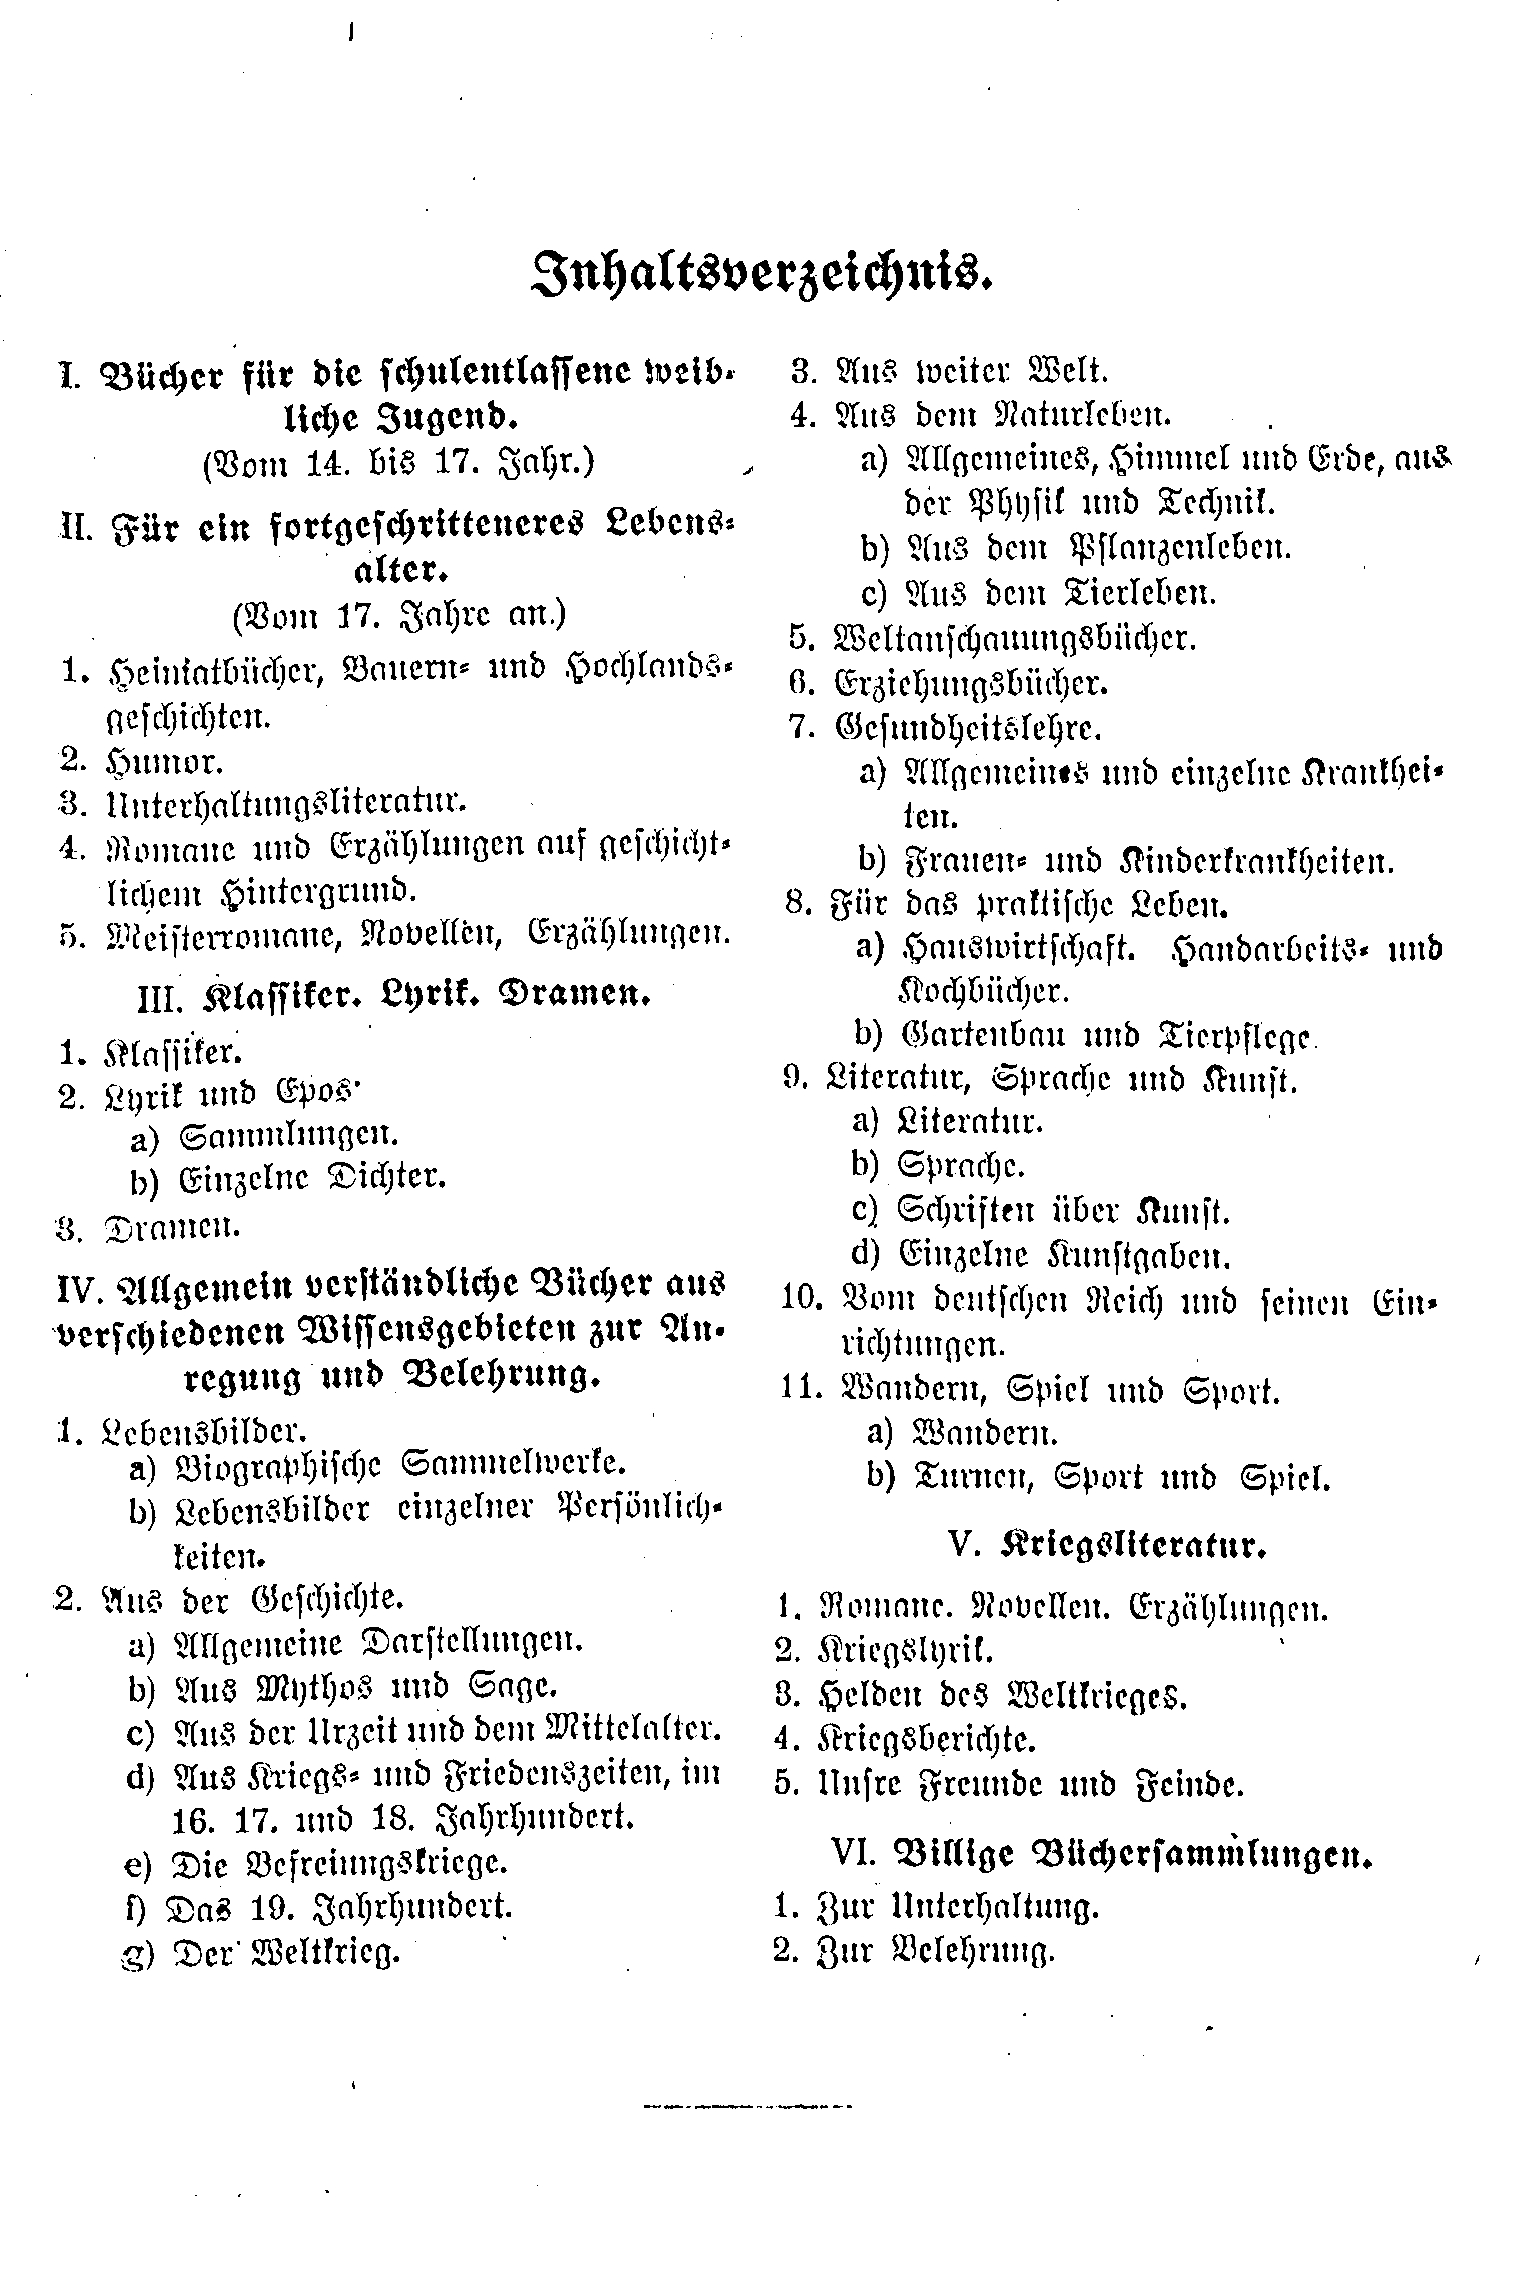
\includegraphics{img/buecherliste_arbeiterinnen_1.jpg}
\caption{Verein zur Verbreitung guter volkstümlicher Schriften 1918a:
37.}
\end{figure}

\begin{figure}
\centering
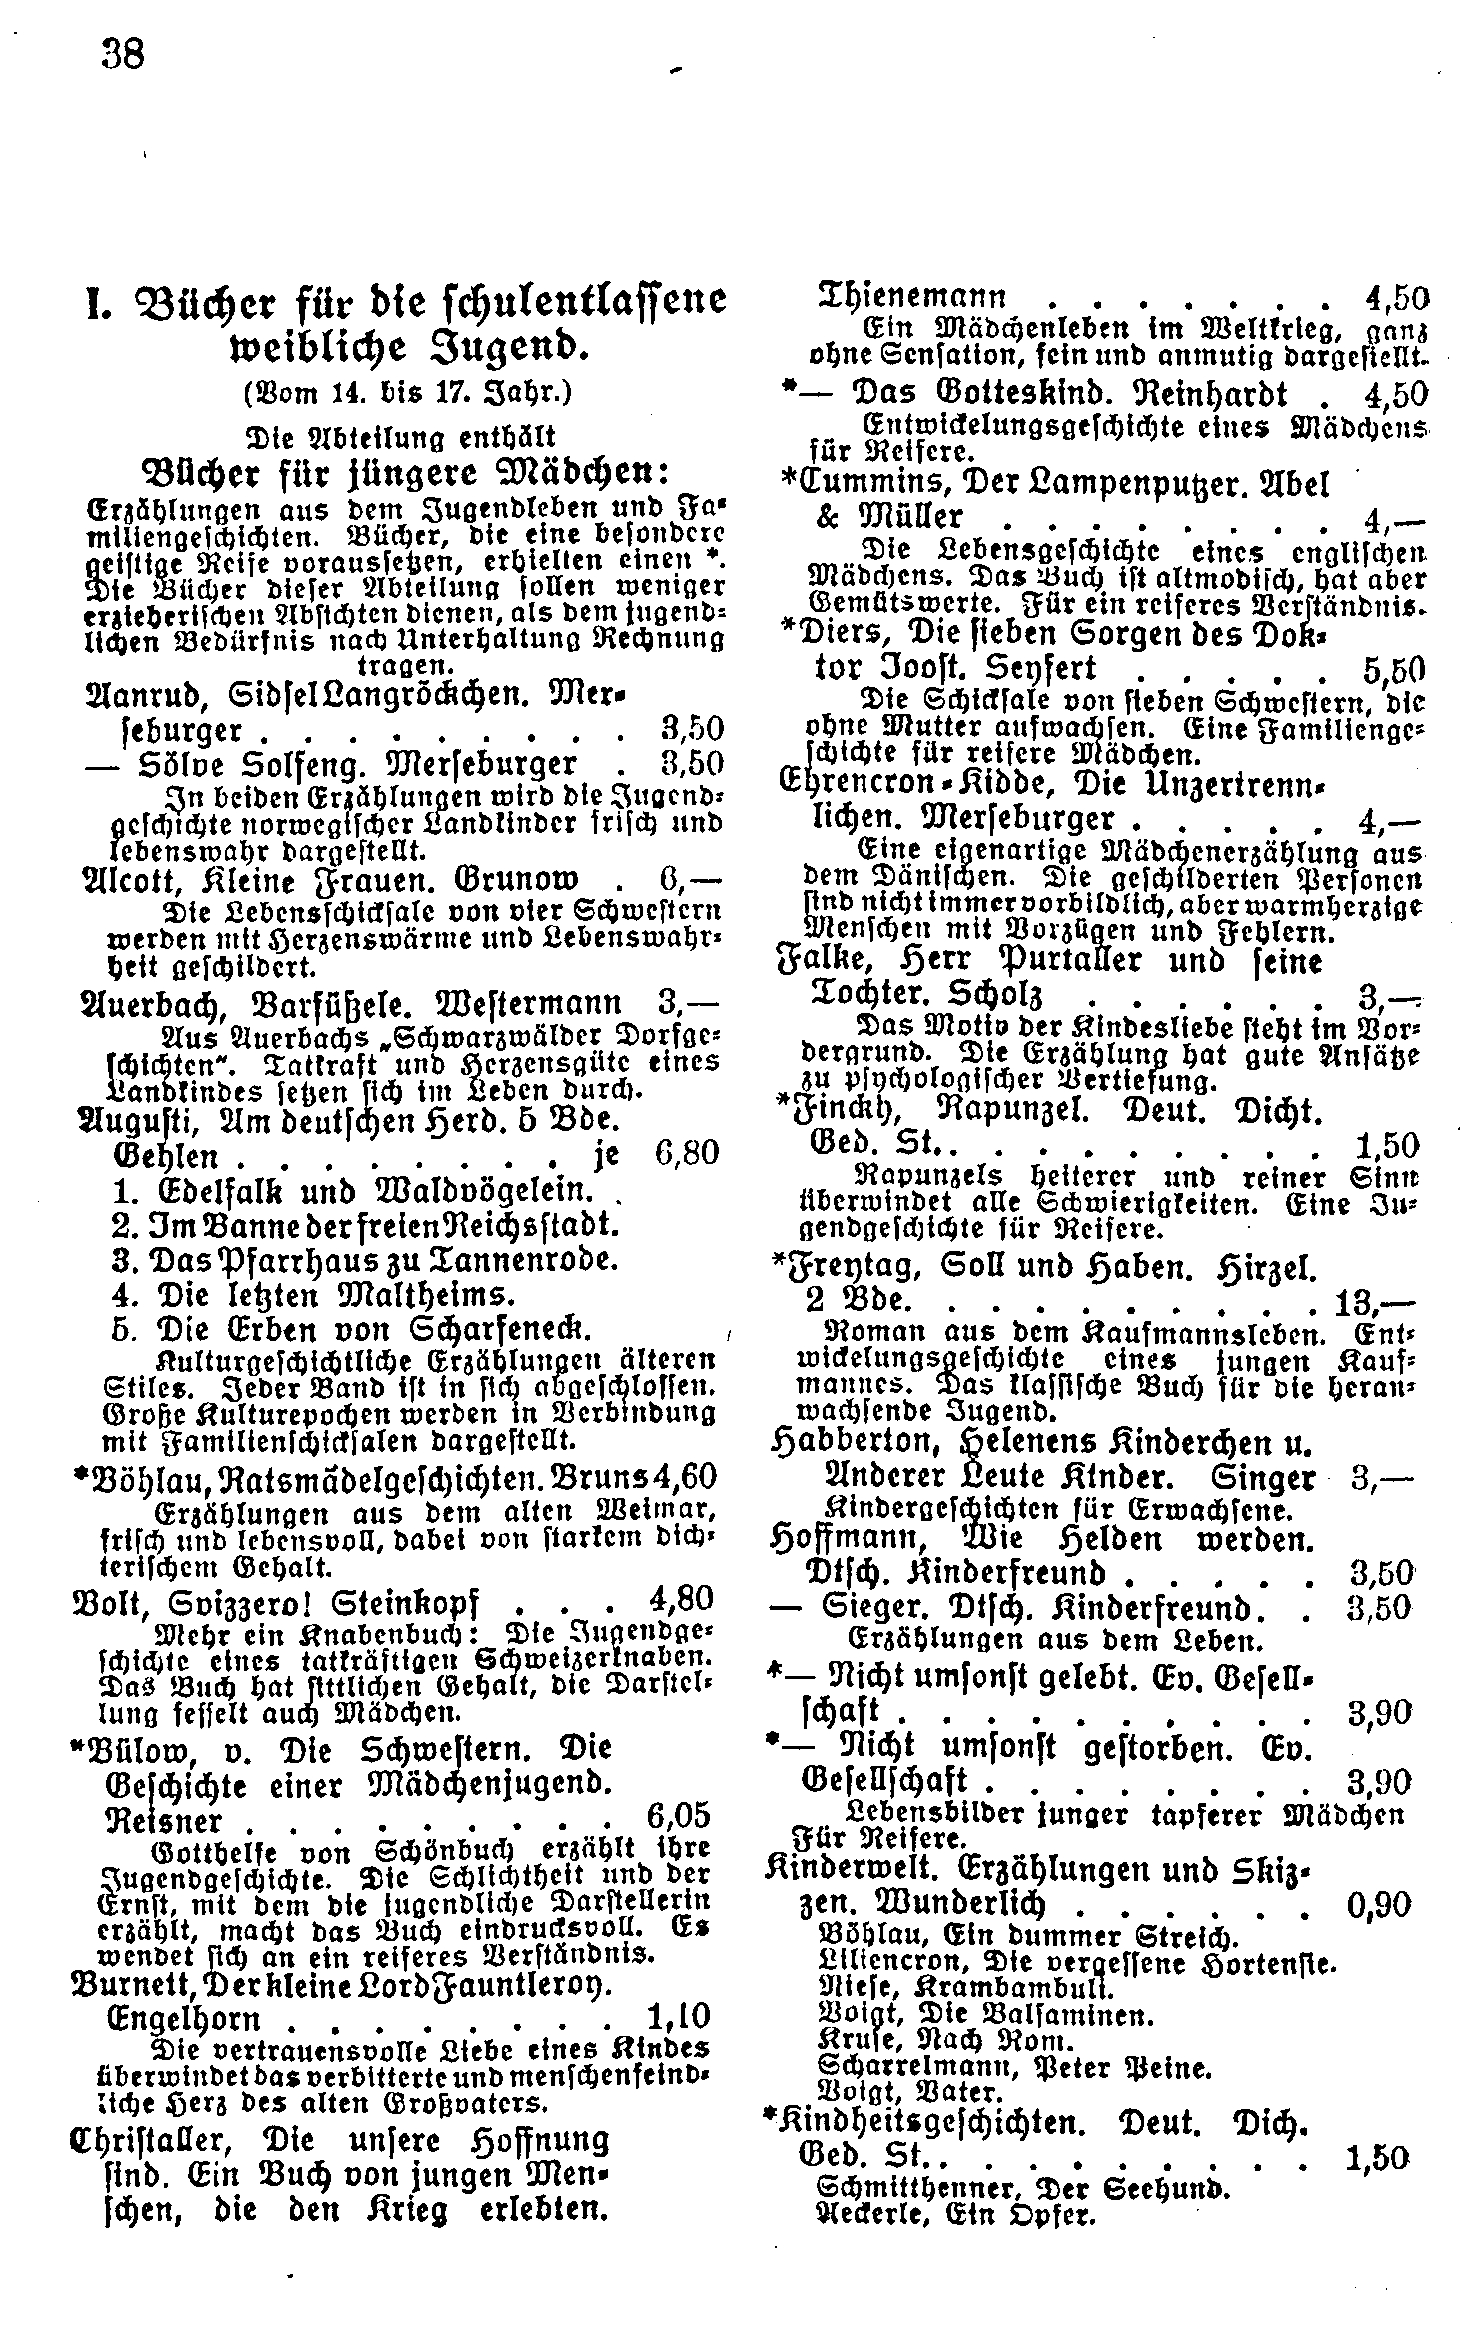
\includegraphics{img/buecherliste_arbeiterinnen_2.jpg}
\caption{Verein zur Verbreitung guter volkstümlicher Schriften 1918a:
38.}
\end{figure}

\hypertarget{verweis-zum-eingangszitat}{%
\subsection{2.3 Verweis zum
Eingangszitat}\label{verweis-zum-eingangszitat}}

Mit dem bis hierher dargestellten Kontext lässt sich das Zitat, welches
dem Artikel vorangestellt wurde, noch einmal neu lesen. In dem Text, aus
dem es stammt, stellt Franz Schriewer (hier in Doppelfunktion als
Vertreter des Vereins \emph{Grenzbüchereiarbeit e.V.} und als Leiter der
\emph{Zentrale für Nordmarkbüchereien}) direkt am Anfang der
nationalsozialistischen Herrschaft dar, welche Prinzipien die
«Grenzbüchereiarbeit» hat, was sie bis dato geleistet hatte und was sie
jetzt im Rahmen des «neuen Staates» leisten würde. Der Text ist in
gewisser Weise einer, mit dem sich der \emph{Grenzbüchereiarbeit e.V.}
als Verbündeter des neuen Regimes darstellt.

Im Zitat selber finden sich nun sowohl büchereipädagogische als auch
völkische Prinzipien. Zuerst betont Schriewer völkische Vorstellungen
vom Volk als einem «Gesamtkörper», das sich gegenüber anderen Völkern
«behaupten» müsse. Dafür müsse es seine «Kräfte voll entwickeln», und
zwar «harmonisch». Aber: In einer Grenzlage sei es bedroht, weil es mit
anderen Völkern in Kontakt sei. Deshalb müsse gerade dort «die bedrohte
völkische Lebenskraft von der kulturellen Seite her so pfleglich wie
möglich behandelt {[}werden{]}». (Schriewer 1933a: 7) Während er dies
als allgemeine Regel für alle Völker postuliert, geht er dann im zweiten
Teil des Zitates explizit auf das deutsche Volk ein und behauptet, dass
«hierfür das deutsche Buch als {[}...{]} Rückhalt und Träger deutscher
Kultur planmäßig einzusetzen {[}sei{]}». (Schriewer 1933a: 8) Bücher
hätten eine direkte Wirkung, sowohl «befruchtend oder auch
zerstörerisch». Das ist eine Grundüberzeugung der Büchereipädagogik, die
Schriewer hier explizit in den Zusammenhang mit einem völkischen
Programm stellt. Und, so wie die völkische Bewegung (aber auch die
Büchereipädagogik) sich als modern und vorwärtsgerichtet verstand, geht
es ihm gerade nicht um eine Rückkehr zu Traditionen, sondern um eine
explizite Planung und Aufbauarbeit, also um den Einsatz moderner
pädagogischer und staatlicher Instrumente: «Es kann sich also bei der
Pflege des Buches in den Grenzgebieten immer nur um einen kulturell und
pädagogisch geregelten Einsatz handeln, wozu öffentliche, kräftig
entwickelte Büchereien notwendig sind.» (Schriewer 1933a: 8)

Das Zitat ist also keine allgemeine Äusserung zur Bedeutung von
Büchereien oder des Lesens im Allgemeinen, sondern es ist eine explizit
im Kontext von völkischem Denken und Büchereipädagogik stehende
Forderung, Büchereien zielgerichtet einzusetzen -- und zwar
zielgerichtet zur Erreichung der Ziele des nationalsozialistischen
Staates (der damals, 1933, noch nicht mit dem Holocaust, dem Zweiten
Weltkrieg und weiteren Verbrechen in Zusammenhang stand, aber dessen
Ziele und Gewaltförmigkeit schon klar sichtbar waren). Wie weiter unten
(Kapitel 4.) sichtbar wird, stellte dieser Text keine neue Stufe im
Denken der Grenzbibliotheksarbeit (oder Schriewers) dar, sondern war
eher eine Zusammenfassung dessen, was schon in den Jahren zuvor
geschrieben wurde.

\hypertarget{grenzbuxfcchereiarbeit-wuxe4hrend-der-weimarer-republik}{%
\section{3. Grenzbüchereiarbeit während der Weimarer
Republik}\label{grenzbuxfcchereiarbeit-wuxe4hrend-der-weimarer-republik}}

\hypertarget{der-verein-zur-verbreitung-guter-volkstuxfcmlicher-schriften}{%
\subsection{\texorpdfstring{3.1 Der \emph{Verein zur Verbreitung guter
volkstümlicher
Schriften}}{3.1 Der Verein zur Verbreitung guter volkstümlicher Schriften}}\label{der-verein-zur-verbreitung-guter-volkstuxfcmlicher-schriften}}

Im Folgenden wird es nun vor allem um den Verein
\emph{Grenzbüchereidienst e.V}. und seine Entwicklung gehen. Gegründet
wurde dieser aber unter einem anderen Namen, nämlich \emph{Verein zur
Verbreitung guter volkstümlicher Schriften}. Jener wurde 1914 während
des Ersten Weltkrieges in Berlin mit dem Ziel etabliert, den (deutschen)
Soldaten an der Front Bücher zu schicken. Später wurden auch kleine
Büchereien für Soldaten aufgebaut. Ziel war es, so ein Text von 1917,
welcher diese Arbeit vorstellt, «allen Feldgrauen, die sich darnach
{[}sic!{]} sehnen, Freunde und Anregung zu bringen». (Lindmaier 1917:
10) Spätestens Juli 1918 (also noch vor dem Ende des Ersten Weltkrieges)
begann der Verein auch, sich für die Verbreitung «guter Schriften» in
den unteren Schichten des Volkes als zuständig zu erklären. (Verein zur
Verbreitung guter volkstümlicher Schriften 1918b) Der Verein war gut in
die Strukturen von Militär und deutscher Oberschicht eingebunden. Auf
der Umschlagseite der ersten Ausgabe der \emph{Mitteilungen} des Vereins
findet sich eine Aufstellung von Vorstand und Beirat. (Verein zur
Verbreitung guter volkstümlicher Schriften 1917b) Vorsitzender ist ein
Militär (Generalleutnant von Schubert, wohl Richard von Schubert), die
anderen Mitglieder (alles Männer) werden als Oberregierungsräte,
Kommerzienräte, Verlagsbuchhändler, Direktoren und so weiter bezeichnet.
Dies ermöglichte Zugang zu Mitteln, aber auch zur tatsächlichen
Verbreitung von Büchern und Broschüren an der Front. Der Verein
unterhielt eine Zentrale in Berlin, von der aus sowohl während des
Weltkrieges als auch später hunderttausende Bücher verschickt wurden und
weitere Arbeit geleistet wurde.

Die Existenz eines solchen Vereins war an sich nicht für Deutschland
spezifisch. Dies passierte gleichzeitig in anderen Ländern.\footnote{Bekannt
  ist zum Beispiel die \emph{Schweizerische Soldatenbibliothek}, die
  dann nach 1918 zur \emph{Schweizerischen Volksbibliothek} -- der
  heutigen \emph{Stiftung Bibliomedia Schweiz} -- umgewandelt wurde.
  (Escher 1922)} Auch, dass zu Beginn des Ersten Weltkrieges von
Angehörigen der Elite Vereine gegründet wurden, die für die breite Masse
tätig wurden, war nicht ungewöhnlich. Zu Beginn des Krieges gab es eine,
in der Forschungsliteratur immer wieder thematisierte, breit in der
Gesellschaft geteilte Vorstellung einer «Gemeinsamkeit des Volkes» über
die Schichten hinweg. Dieses wurde später, auch gerade in der völkischen
Bewegung, zum «Augustereignis» mythologisiert (weil es im August 1914
stattfand). Dieses Zusammengehörigkeitsgefühl hatte tatsächliche
Auswirkungen, wie die Gründung solcher Vereine.

Was den Verein etwas aus ähnlichen Unternehmungen (aber auch nicht
allen) hervorhebt, ist, dass er nach dem Ende des Krieges weiter
existierte. Er verschob seinen Tätigkeitsbereich (Verein zur Verbreitung
guter volkstümlicher Schriften 1921b), aber erst 1928 änderte er seinen
Namen in \emph{Grenzbüchereidienst und Bildungspflege e.V.} (Scheffen
1928b). 1933 dann wurde diese Name verkürzt zu \emph{Grenzbüchereidienst
e.V.} (Scheffen 1933), der dann bis zum Ende des Vereines mit dem
Untergang des NS-Staates 1945 beibehalten wurde. Während dieser Zeit
veröffentlichte der Verein immer wieder einmal Listen seiner
Vorstandsmitglieder. (Zum Beispiel Anonym 1922) Zumindest bis zum Beginn
der 1930er Jahre waren dies immer wieder Vertreter der
gesellschaftlichen, politischen und wirtschaftlichen Elite,
beispielsweise Ernst von Borsig, damals Vorsitzender der Vereinigung der
Deutschen Arbeitgeberverbände sowie des Reichsverbandes der Deutschen
Industrie, der auch als Vorsitzender des Vereins fungierte (wobei die
eigentliche Arbeit wohl vom «Geschäftsführenden Vorsitzenden» Wilhelm
Scheffen geleistet wurde).

Diese ganze Zeit über gab der Verein unregelmässig \emph{Mitteilungen}
heraus, die gleichzeitig Informationsblatt und Werbemittel waren. Der
konkrete Name änderte sich mit den Umbenennungen des Vereines, aber
sowohl das Format als auch die Nummerierung wurden beibehalten. In
diesen \emph{Mitteilungen} dokumentierte der Verein seine Zielsetzungen
und Denkweise selbst. Sie stellen die Hauptquelle für die folgenden
Kapitel dar.

Gleichwohl war dies, wie schon erwähnt, nicht der einzige Ort, an dem
der Verein sichtbar wurde. Während die konkreten Büchersendungen, die er
verschickte, heute nicht mehr vorhanden sind, ist er in den 1920er und
1930er Jahren kontinuierlich in der Fachpresse des Volksbüchereiwesens
vertreten. Wichtige Vertreter*innen des Vereines waren zudem, wie weiter
unten geschildert wird, in wichtigen Positionen in diesem Büchereiwesen
beruflich engagiert. Sie publizierten sowohl über die Arbeit des Vereins
als auch im Rahmen ihrer beruflichen Tätigkeit, wie schon für Franz
Schriewer erwähnt. Gleichzeitig hatte der Verein offenbar immer wieder
Personen, die bei ihm angestellt waren oder zumindest explizit für ihn
arbeiteten, wie das Ehepaar Wilhelm Scheffen und Luise Scheffen-Dörring.

Die Arbeit des Vereines war schon zu Beginn, wie am ersten Namen
sichtbar wird, an büchereipädagogischen Prinzipien ausgerichtet. Die
Schriften, die verschickt wurden, sollten «gut» sein, aber gleichzeitig
auch «volkstümlich», dass heisst hier für Menschen aus den unteren
Sozialschichten zugänglich. Schon in der ersten Nummer der
\emph{Mitteilungen} (1917) wird ein «Verzeichnis guter billiger
Literatur» (Verein zur Verbreitung guter volkstümlicher Schriften 1917a:
17) veröffentlicht, dass es ermöglichen sollte, die richtigen Bücher
auszuwählen, falls man solche «ins Feld senden {[}will{]}» (Verein zur
Verbreitung guter volkstümlicher Schriften 1917a: 17). Es wird nicht
gesagt, nach welchen Kriterien diese Auswahl getroffen wurde, ausser,
dass es Bücher seien, «die den Leser fesseln, erfreuen und bereichern
können» (Verein zur Verbreitung guter volkstümlicher Schriften 1917a:
17) und die leicht, handlich, aber auch kostengünstig wären. Es wird
geschrieben, dass keine religiös-erbaulichen Schriften aufgenommen
wurden. Ansonsten ist es eine Liste, die 14 Seiten lang und in zwei
Spalten gesetzt, Bücher aus verschiedenen Kategorien kurz mit
bibliographischen Angaben, Preis und manchmal ganz kurzen
Erläuterungen\footnote{Zum Beispiel zu Marie von Ebner-Eschenbach (ohne
  Datum): \emph{Ein Buch, das gern ein Volksbuch werden möchte} (Einer
  Auswahl der dann gerade verstorbenen Dichterin): «Schöne Erzählungen
  aus dem Volksleben. Soziales Gefühl ist mit starkem sittlichen Gehalt
  verbunden. Inhaltlich fesselnd.» (Verein zur Verbreitung guter
  volkstümlicher Schriften 1917a: 19).} aufzählt. Aber es ist von den
Formulierungen her klar, dass hier wohl ähnliche Prinzipien angelegt
wurden, wie bei den Listen, die direkt von Volksbüchereien erstellt
wurden. Dies wird nur die erste von vielen Listen sein, welche der
Verein im Laufe der Jahre erstellen und dann kostenlos an alle
Interessierten verschicken wird.

\hypertarget{verbindung-von-vuxf6lkischer-ideologie-und-buxfcchereipuxe4dagogik}{%
\subsection{3.2 Verbindung von völkischer Ideologie und
Büchereipädagogik}\label{verbindung-von-vuxf6lkischer-ideologie-und-buxfcchereipuxe4dagogik}}

1920 -- also erst wieder nach dem Ende des Ersten Weltkrieges, aber auch
nach der Unterzeichnung des Versailler Vertrages, der Revolution in
Deutschland und dann der Etablierung der Demokratie -- erschien dann die
dritte Nummer der \emph{Mitteilungen}. Sie begann gleich mit einem
Artikel über «Grenzmarkbüchereien», welcher in gewisser Weise die
weitere Stossrichtung des Vereins vorgab. (Scheffen 1920)

\begin{quote}
«Millionen von Deutschen sind durch den Friedensschluß politisch fremden
Staaten eingegliedert oder stehen in den Abstimmungsgebieten unter
fremder Aufsicht. Wir können das nicht hindern.» (Scheffen 1920: 1)
\end{quote}

Scheffen bezieht sich hier auf die Ergebnisse des Ersten Weltkrieges,
auf den Versailler Vertrag und auf die 1920 noch bevorstehenden
Volksabstimmungen, zum Beispiel in Oberschlesien oder dem Saargebiet, in
denen die Bevölkerung darüber entscheiden konnte, welchem Staat die
jeweiligen Gebiete zugehören sollten. Dabei blickte er nur auf die
betroffenen Menschen, die er als «Deutsche» definierte (und nicht zum
Beispiel die, welche in Oberschlesien lebend, sich selbst als polnisch,
als schlesisch oder noch anders verstanden). Er sieht dies offenbar auch
nicht als Ergebnis eines Krieges an, den das Deutsche Reich, neben den
meisten anderen beteiligten Staaten, aktiv als Angriffskrieg geführt
hatte. Dies war 1920 in Deutschland (und Österreich) eine in vielen
Milieus verbreitete Haltung. Aber im Rahmen der völkischen Bewegung
blieb dies auch über die folgenden Jahre hinweg die bestimmende
Interpretation. In seinem Artikel schliesst Scheffen eine völkische
Deutung an, mit dem er Völker als gegeneinander kämpfende Einheiten
versteht und unterstellt dabei «anderen Völkern» einen Plan.

\begin{quote}
«Zugleich wird man versuchen, diese unsere deutschen Brüder und
Schwester allmählich einer fremdländischen Kultur zu unterwerfen. Das
darf nimmermehr geschehen. Mit aller Kraft setzten wir uns dafür ein,
dass bei ihnen deutsche Sprache, deutsche Sitte, deutsche Kultur weiter
gepflegt und so deutsches Wesen für sie selbst und für Kind und
Kindeskind kräftig erhalten werden.» (Scheffen 1920: 1)
\end{quote}

Eine Eigenheit des völkischen Denkens, immer «vom eigenen Volk»
ausgehend zu denken, wird in diesem Zitat deutlich: Die Situation wird
als Gefahr für das «deutsche Volk» dargestellt, ohne auch nur zu
thematisieren, wie dies bei einem anderen Ausgang des Krieges für
Angehörigen anderer Völker gewesen wäre. Zudem ist es für Scheffen
offenbar undenkbar, das der «Wechsel» von Menschen von einem Volk zum
anderen (oder die Ausbildung von Identitäten «zwischen» zwei Völkern)
ein normaler Vorgang sein könnte, der nicht unbedingt durch Zwang oder
Verführung erreicht werden muss. Er kann es sich offenbar nur als Kampf
anderer Völker gegen das deutsche Volk vorstellen. Wie oben geschildert,
ist im völkischen Denken schon die Vorstellung, dass Angehörige
verschiedener «Völker» in einem Staat zusammenleben können, nicht
wirklich akzeptabel. Wenn, dann immer nur als Kampf.

Alsdann ordnet er die Aufgabe des Vereins, der sich jetzt auf den Aufbau
von Büchereien für «Deutsche» in den Grenzgebieten konzentrieren will,
in dieses Denken ein.

\begin{quote}
«Neben Theateraufführungen und Vorträgen, neben deutschen Liedern und
deutscher Kunst ist das deutsche Buch einer der wichtigsten
Kulturfaktoren zur Erhaltung und Vertiefung deutschen
Volksbewusstseins.» (Scheffen 1920: 1)

«Ein Kampf auf Leben und Tod um das Deutschtum hat in den Grenzmarken
eingesetzt. Der Geist unserer deutschen Dichter und Denker muß in diesem
Kampfe helfen, der Geist eines Goethe, Schiller, Fichte, Eichendorff,
Hebbel, Jeremias Gotthelf, Reuter, Gustav Freitag, Raabe, Riehl,
Lienhard. In fast allen Briefen aus den abgetretenen und besetzten
Gebieten kommt neben dem Dank die Bitte zum Ausdruck, weiter zu helfen.
Dabei hat eine große Zahl von Anträgen noch nicht berücksichtigt werden
können. Große Mittel sind bei den teuren Bücherpreisen erforderlich,
aber unser Verein muß und will diese ihm gestellte Aufgabe durchführen.
Dorf für Dorf, Stadt für Stadt müssen mit deutschen Büchereien versorgt
werden. Wer hilft mit?» (Scheffen 1920: 5)
\end{quote}

Abgeschlossen wird der Text dann mit zwei weiteren Listen von Büchern,
die hier als «Musterliste einer Ostmarken-Bücherei» beziehungsweise
«Musterliste einer Westmarken-Bücherei» bezeichnet werden und jeweils
100 Titel enthalten. Im Zitat wird deutlich, wie in diesem Denken ein
Kanon deutscher Autoren (fast nie Autorinnen) konstruiert wird. Wie alle
Kanons ist auch dieser ein Konstrukt, aber eines, das sich sichtlich an
bürgerliche Vorstellungen von deutscher Kultur anlehnt. Gerade die
Integration von Goethe und Schiller zeigt, dass es dabei nicht immer um
den konkreten Inhalt der Schriften geht -- beide plädierten selber
bekanntlich humanistisch für ein «Weltbürgertum». Goethe legte unter
anderem mit dem «West-östlicher Divan» einen Gedichtband vor, der
explizit ein muslimisches lyrisches Ich hat und islamische Kultur
schildert. Schillers «Wilhelm Tell» wurde auch schon in einem anderen
Land, der Schweiz, als Teil des eigenen Kanons herangezogen. Das alles
sollte sie eigentlich dem völkischen Denken nach ausschliessen. Aber,
wie schon gesagt, war dieses Denken von niemals aufgelösten
Widersprüchen geprägt.

Bedeutsam an diesem Text ist, dass hier mit den «Musterlisten» gezeigt
wird, dass sich der Verein weiter im Rahmen der normalen Arbeit, wie sie
damals auch im Volksbüchereiwesen geleistet wurde, bewegte. Er war auch
keine Ausnahme, sondern der erste in einer langen Reihe ähnlich
argumentierender Beiträge. Im gleichen Heft der \emph{Mitteilungen}
findet sich zum Beispiel ein Text über «Das Buch zur Pflege des
Deutschtums in besetzten Gebieten» (Winker 1920\footnote{«Deutsche
  Heimat in Ost und West ist in Gefahr. Alte Kultur im Westen, neues
  Kolonistenland im Osten soll uns entrissen werden: wertvollstes
  Ländergebiet, das durch deutsche Arbeit emporgehoben ist. Fremdes
  Wesen schleicht umher und nimmt Tausenden den Trieb zum Vaterlande.
  Gesinnungslosigkeit bringt Vorteil. Kein gemeinsames deutsches Lied;
  keine vaterländische Feierstunde; kein Regimentsmarsch einer deutschen
  Kapelle mehr draußen auf der Gasse. Wer da nicht fest im deutschen
  Heimatlande wurzelt, kommt in Gefahr. Und wir sollen tatenlos zusehen?
  Eins können wir tun: wir {[}sic!{]} können Bücher senden, die von
  deutscher Heimatseele zeugen. Im Buch haben die besten unseres Volkes
  ihre Gedanken und Gefühle niedergelegt. Es muß nun hinauswandern in
  unsere Marken als Freund und Tröster; muß Zeuge sein für deutsche
  Kultur, deutsches Wissen und deutsche Seele.\\
  Da erwächst den Volksbüchereien eine ungeheure Aufgabe. Sie sind in
  erster Linie dazu berufen, vertiefte Heimatkenntnis zu vermitteln;
  ihre Aufgabe ist bewußte Pflege der Stammeseigenart und starker
  stolzer Heimattreue. Wer die Heimat liebt, liebt das Vaterland.
  {[}\ldots{]} Will man also den Weg zum Herzen des einfachen Menschen
  finden, so muß man Bücher wählen, in denen die Seele der Heimat
  schwingt. Große Bünde sind heuer entstanden, um ein neues Wurzelfassen
  in heimatlichem Boden zu fördern. Unter ihren Mitteln nimmt das Buch
  eine bevorzugte Stelle ein.» (Winker 1920: 8f.)}) sowie ein weiteres
Verzeichnis «Literatur für Grenzmarkenbüchereien» (Verein zur
Verbreitung guter volkstümlicher Schriften 1920). Auch dieses
Verzeichnis führt auf jetzt über 20 Seiten, zweispaltig gesetzt, Bücher
auf, geordnet nach einer einfachen Systematik (zum Beispiel. «B.
Dichtung, I. Lyrik und Epos, II. Drama, III. Klassiker») und teilweise
mit kurzen Quellenangaben. Dass diese Liste im Rahmen der
Büchereipädagogik als Hilfsmittel für Bibliothekar*innen gedacht ist,
zeigt sich daran, dass eine Anzahl der Bücher zusätzlich mit einem *
gekennzeichnet wurde, welche eine «größere geistige Reife der Leser
{[}voraussetzen{]}» (Verein zur Verbreitung guter volkstümlicher
Schriften 1920: 23). Wieder ist nicht klar, nach welchen Kriterien die
Bücher ausgewählt wurden, aber eine Durchsicht der Kommentare und Titel
lässt vermuten, dass ein Ziel war, dass sie in Deutschland spielen oder
aber einen «Kampf auf Leben und Tod um das Deutschtum» (Scheffen 1920:
5) irgendwie widerspiegelten. In einem Text, der dann ein Jahr später
erscheint, werden in den \emph{Mitteilungen} «{[}g{]}ute volkstümliche
Schriften aus den letzten Jahren» (Reinhold 1921: 37) besprochen, in
denen das explizit zum Kriterium erhoben wird.

Dieser grundsätzlichen Linie, die bei Scheffen 1920 angelegt ist, folgte
der Verein dann die gesamte Zeit der Weimarer Republik über. Er wurde
auf der einen Seite immer radikaler, was seine völkischen Grundideen
anging und gleichzeitig -- wie im nächsten Abschnitt gezeigt wird -- in
der konkreten Arbeit immer professioneller. Herausstechend aus den
Beiträgen, die der Verein in seinen \emph{Mitteilungen} publizierte, ist
einer von 1929. (König 1929) Der Text selber hat gar keine Verbindung zu
irgendeiner Form von Büchereiarbeit oder Literatur, sondern stellt
völkische Überzeugungen gedrängt zusammen. Seinen Abdruck in den
\emph{Mitteilungen} kann man als programmatisch verstehen. Er beginnt
gleich mit einer Darstellung der «Verhältnisse» in Europa:

\begin{quote}
«Im Deutschen Reich wohnen rund 64 Millionen Menschen. Sie sind bis auf
geringe Bruchteile Angehörige des deutschen Volkes, die Zahl der
Angehörigen fremder Völker hat infolge der Abtretungen gewaltig
abgenommen. {[}\ldots{]} Dafür aber leben 30 bis 40 Millionen
volksdeutsche Menschen außerhalb des Deutschen Reiches als Staatsbürger
anderer Staaten. Wir Deutschen sind in Europa allein in 20 von 30
Staaten seit alters seßhaft. Wir sind Staatsvolk in fünf Staaten: Reich,
Österreich, Danzig, Luxemburg, Liechtenstein; Mitträger der
Staatlichkeit in einem Staate: Schweiz; und Mitträger in einer
Teilrepublik Sowjetrußlands: Wolga-Republik; in 13 Staaten sind wir
Minderheitenvolk: Belgien, Frankreich, Italien, Jugoslawien, Ungarn,
Rumänien, Tschechoslowakei, Polen, Litauen, Lettland, Estland,
Sowjetrußland, Dänemark, wobei wir von dem zu einem westgermanischen
Sondervolk gewordenen Holländertum und den Flamen Belgiens und
Frankreichs absehen wollen. Das deutsche Volk ist eine all diese Staaten
überwölbende Gesamtpersönlichkeit.» (König 1929: 26)
\end{quote}

Im Text wird weiterhin behauptet, dass erst nach dem Ersten Weltkrieg in
breiten Kreisen die «Bedeutung» der Volksidentität erkannt worden wäre.
Jetzt würde es darum gehen, diese Identität zu stärken, insbesondere, da
dies von «anderen Völkern» auch gemacht würde. Der Text behauptet
explizit, dass es einen Unterschied zwischen Staat und Volk gäbe, das
aber beide existieren würden. Er deutet an, dass die Staaten sich eher
verändern -- also mit der Zeit andere Grenzen haben würden --, als dass
sich Völker verändern. Zudem wird in diesem Text auch gesagt, warum eine
Arbeit «an der Grenze» notwendig wäre:

\begin{quote}
«Die Grenze ist keine Linie, wie wir vor 1914 meinten, durch die links
und rechts klare Verhältnisse geschaffen seien; die Grenze ist Streifen,
ist Saum, ist eine Landschaft, um die politisch und kulturell gerungen
wird; Grenzlandmenschen sind Menschen, die auch seelisch in dem Ringen
der beiden Staaten und Völker darinstehen und daher leicht eine
besondere seelische Struktur, aber auch eine besondere volks- und
staatspolitische Aufgaben erhalten. Bei diesen Menschen besteht
einerseits die Gefahr des Abgleitens von einem zum anderen Volke, von
einem zum anderen Staate, besteht andererseits die Möglichkeit der
Ausbildung besonderen Grenzwissens und Bewußtseins besonderer volks- und
staatspolitischer Verantwortung.» (König 1929: 44)
\end{quote}

Andere Texte des Vereins formulierten dies nicht immer ganz so konkret,
aber all die Schlagworte, die in diesem Text exemplifiziert werden und
auch die dahinterstehenden Ideen finden sich kontinuierlich in den
restlichen Beiträgen angedeutet. «Grenzlandarbeit» wird hier also nicht
als Infrastrukturföderung von potentialarmen Regionen, sondern explizit
als eine Art Unterstützung im Kampf «gegen andere Völker» verstanden.

\hypertarget{konkreter-grenzbuxfcchereidienst}{%
\subsection{3.3 Konkreter
«Grenzbüchereidienst»}\label{konkreter-grenzbuxfcchereidienst}}

Der Verein benutzte seine \emph{Mitteilungen} auch für Berichte über
seine konkrete Arbeit. (Lindmaier 1917, Verein zur Verbreitung guter
volkstümlicher Schriften 1921a, Scheffen 1921, Scheffen 1928a, Weber
1928, Anonym 1928, Weber 1929, Nachtigall 1929, Hesse 1931)
Selbstverständlich sind diese Darstellungen mit Vorsicht zu
interpretieren -- sie sind immer daraufhin ausgelegt, den Verein positiv
darzustellen. Aber man erhält mit ihnen doch einen guten Überblick.

Wilhelm Scheffen gibt in seiner Übersicht vom Dezember 1921 an, dass der
Verein bis dato 314 Büchereien mit 21.124 Büchern aufgebaut hätte.
(Scheffen 1921) Das sind rund 67 Bücher pro «Bücherei». Auch wenn diese
Bestände jeweils vor Ort ergänzt wurden, muss man sie sich also als sehr
klein vorstellen. Zumeist waren es wohl Schränke, in denen sie
untergebracht waren, keine eigenständigen Büchereien. Allerdings war
diese eher kleine Zahl von Büchern im Rahmen der Büchereipädagogik auch
nicht per se negativ -- es ging ja, wie weiter oben dargestellt, darum,
dass Bücher möglichst genau und intensiv gelesen wurden, nicht darum,
dass möglichst viele Bücher konsumiert werden. Weiterhin gibt Scheffen
an, wohin diese Bücher verschickt wurden. Eine Anzahl (40) wurden an
«Flüchtlingsgemeinschaften» abgegeben, weitere 2 in das «frühere
{[}\ldots{]} Schleswig» (Nordschleswig, nach der Volksabstimmung 1920
ein Teil Dänemarks). Die restlichen Bücher gingen in «Grenzgebiete» an
den östlichen Grenzen Deutschlands beziehungsweise Österreichs (2).

Verschickt wurden diese jeweils an Vereine, nicht an die Gemeinden. Er
nennt Heimatvereine, Vaterländische Frauenvereine,
Volksbildungsvereinigungen und Kirchgemeinden sowie, in den
Flüchtlingslagern, das Rote Kreuz. Dies war, wie weiter oben
geschildert, nicht grundsätzlich überraschend. Erst während der 1920er
begann, wie schon erwähnt, eine Entwicklung wirklich Fahrt aufzunehmen,
bei der im DACH-Raum Gemeinden und der Staat an sich Verantwortung für
die Volksbüchereien übernahmen. Ausserhalb einiger grosser Städte (und,
im Fall von Werkbibliotheken, einigen grosser Fabriken) waren es vor
allem Vereine, welche die Büchereien trugen. Der hier besprochene
\emph{Grenzbüchereidienst e.V.} zielte auf den ländlichen Raum, insoweit
gab es auch praktisch keine anderen Strukturen als dort ansässige
Vereine, auf die er sonst aufbauen konnte. Zumal, wieder den Angaben von
Scheffen nach, der Grossteil der Bibliothekar*innen entweder Lehrer (87)
oder Pfarrer (26) waren, gefolgt dann erst von Landwirten (15) und
«sonstigen Personen» (39). Personen mit dem eigenständigen «Beruf»
Bibliothekar*in gab es in diesen Fällen nicht.

Diese Zahl von Bibliothekar*innen (157) stimmt nicht mit den 314
verschickten Büchereien überein. Solche Differenzen finden sich auch
immer wieder in späteren Berichten, wenn konkrete Zahlen genannt werden.
Man kann also davon ausgehen, dass eine ganze Zahl dieser Büchereien
auch nicht lange aktiv betrieben wurde. Der Verein ist sich dem bewusst
und versucht, für eine Kontinuität zu sorgen: «Eine Bücherei hat
freilich nur dann Bestand und behält nur dann ihren Wert, wenn sie
dauernd gepflegt und ergänzt wird. Daher wird zwischen den Empfängern
der Bücherei und unserem Verein eine enge Verbindung herbeigeführt.
Gleich bei der Ueberweisung {[}sic!{]} der Bücherei werden {[}\ldots{]}
‹Leitgedanken zur Einrichtung von Volksbüchereien› mitgeschickt.»
(Scheffen 1921: 5) Im Artikel folgt dann der Text dieser Leitgedanken,
welche darauf hinweisen, dass die Bücherei aktiv betrieben, ergänzt und
ein kurzer Bericht über die Nutzung an den Grenzbüchereidienst geschickt
werden sollte.

Scheffen zitiert aus einigen dieser Berichte, durchweg positiv, und
zeigt eine Statistik zur Benutzung einer dieser Büchereien. Diese ist
gegliedert nach den 50 vorhandenen Büchern sowie danach, ob
Schüler*innen (getrennt nach Knaben und Mädchen), die «Reife Jugend»
(getrennt nach Arbeiter, Arbeiterinnen und Andere) oder «Erwachsene»
(wieder getrennt nach Arbeiter, Arbeiterinnen und Andere) diese jeweils
ausgeliehen hatten. Solche Formen von Statistiken waren zur Zeit der
Büchereipädagogik verbreitet. Es wurde die Ausleihe der einzelnen Titel
oder sehr spezifischer Gruppen angegeben sowie die soziale Schicht der
Leser*innen erhoben, um auf das konkrete Leseverhalten unterschiedlicher
Schichten eingehen zu können. Das hier auf Arbeiter*innen gesondert
geachtet wird, ist mit der Überzeugung zu erklären, dass diese besonders
«gefährdet» wären, nicht völkisch zu denken (sondern «sozialistisch»).

\begin{figure}
\centering
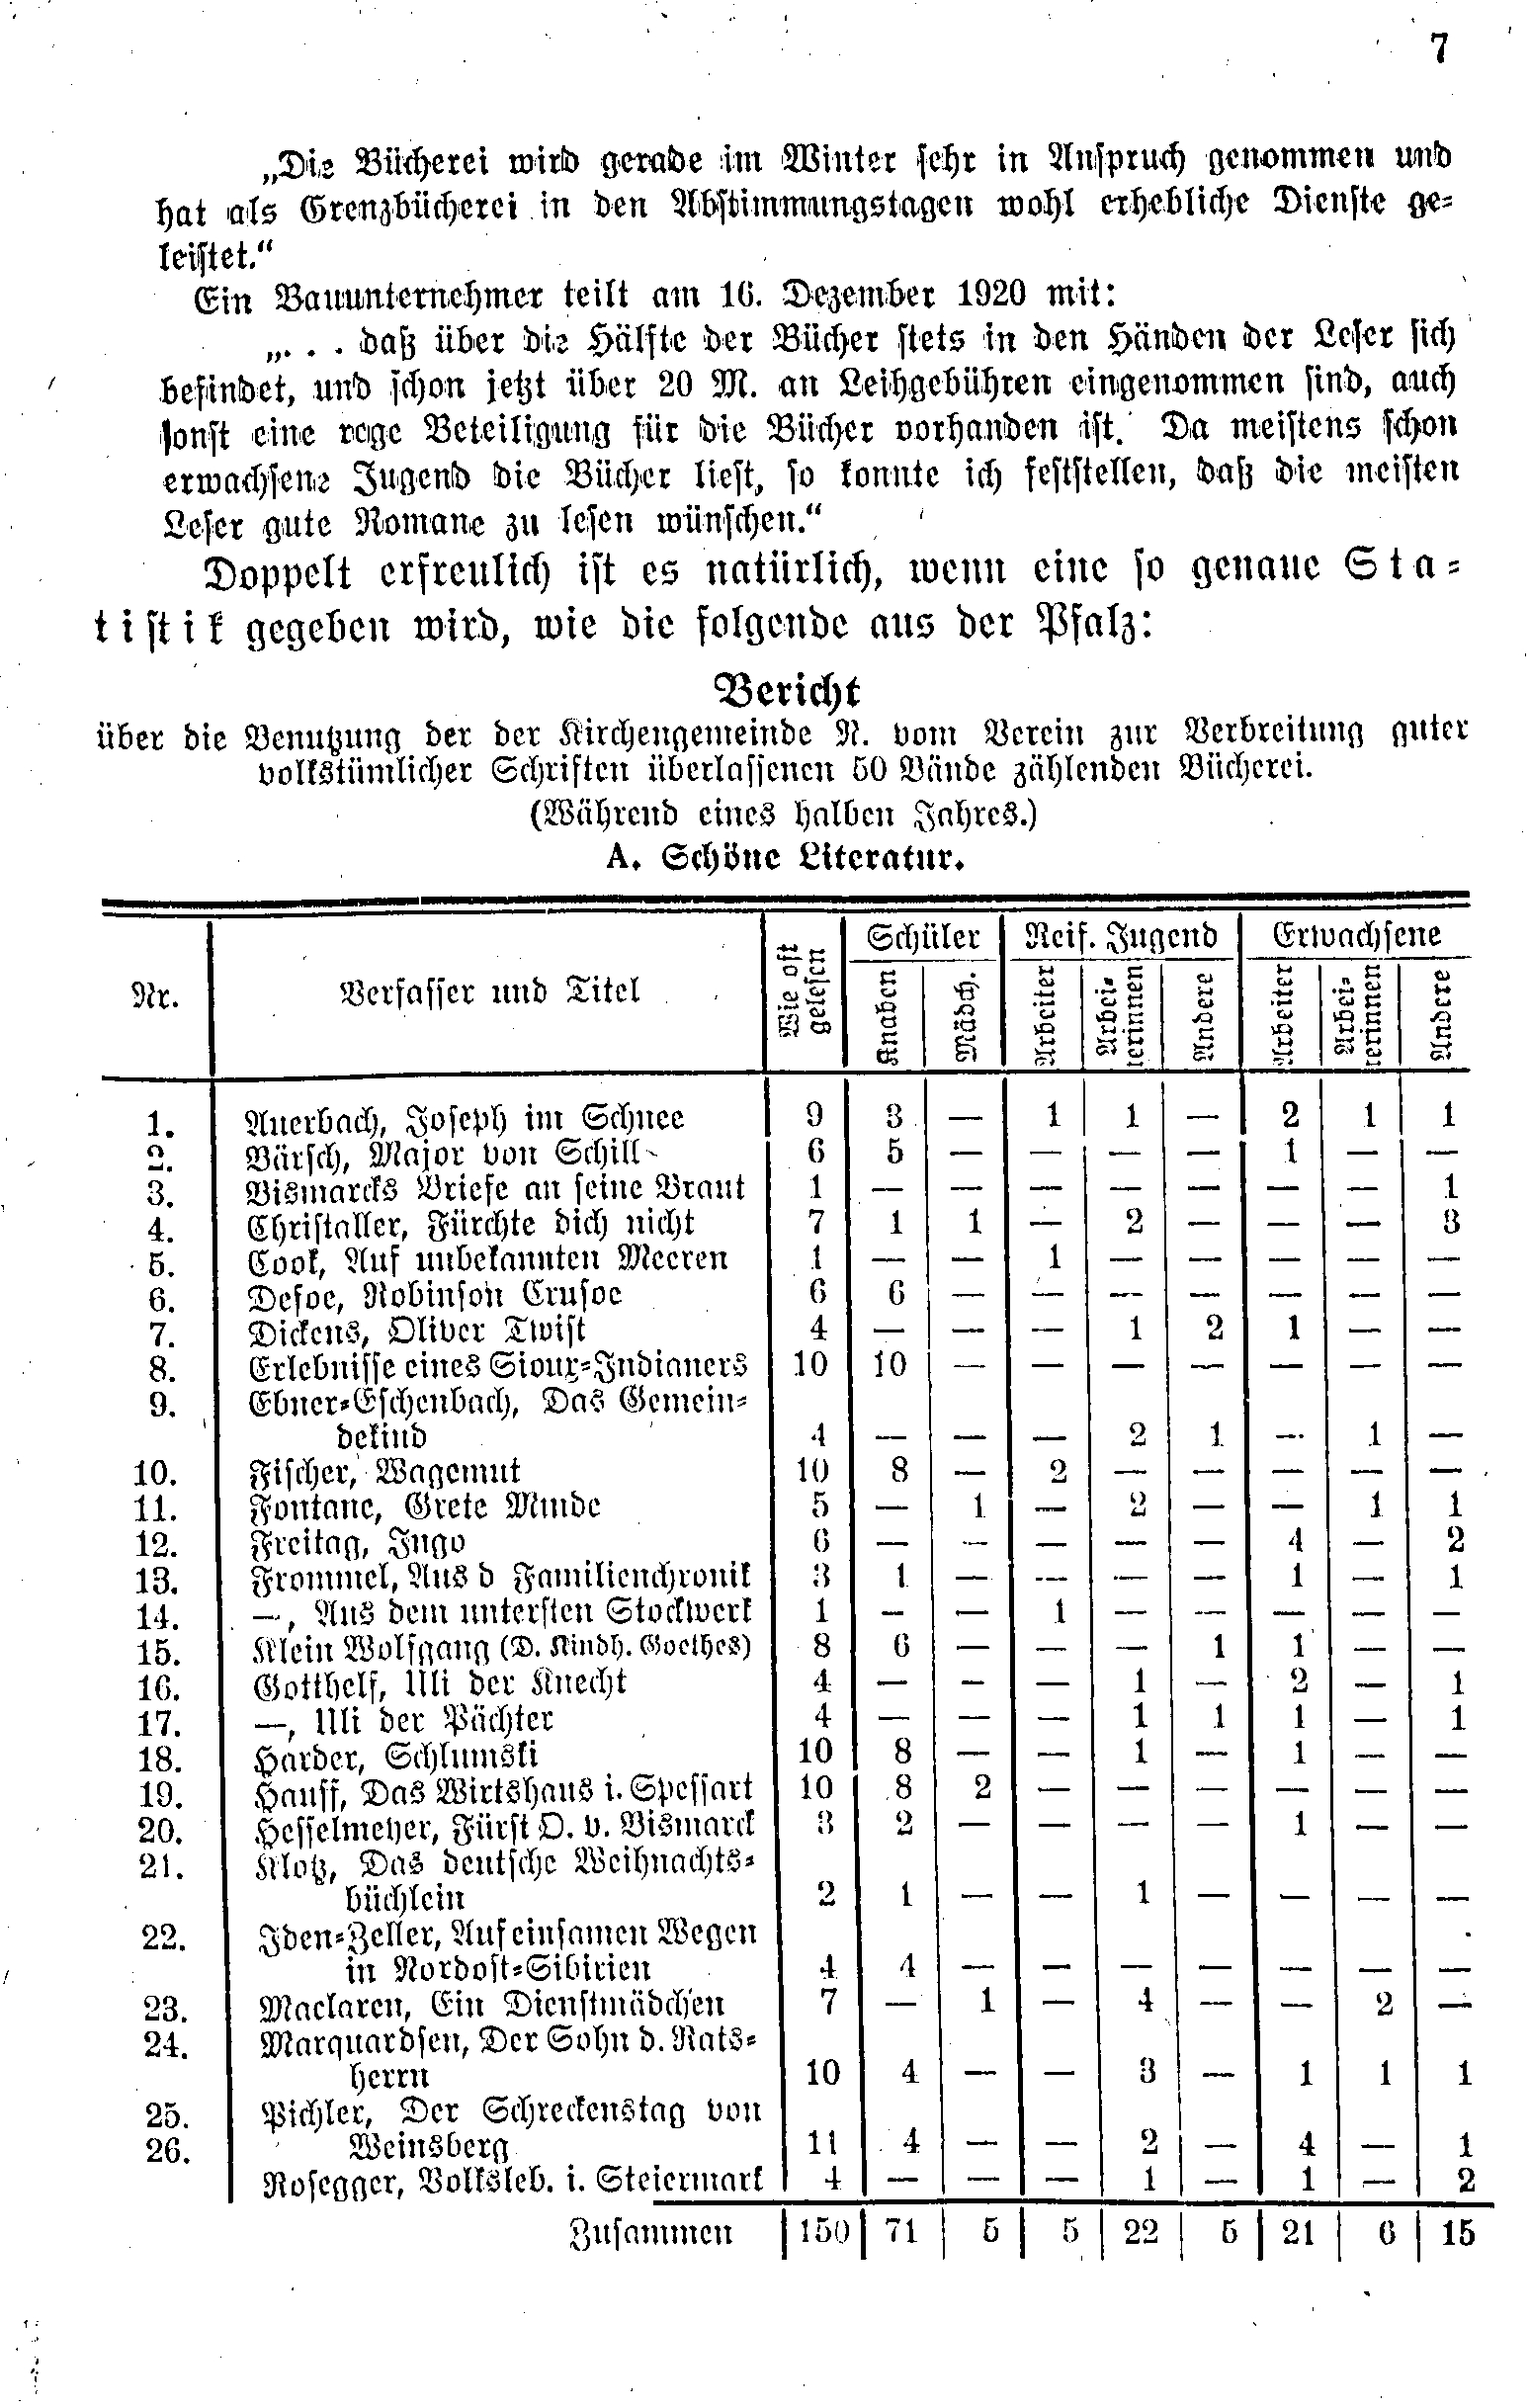
\includegraphics{img/scheffen_statistik_1.jpg}
\caption{Aus Scheffen 1921: 7. Dargestellt wird die Ausleihstatistik der
Bücherei einer Kirchgemeinde (R., «aus der Pfalz»).}
\end{figure}

\begin{figure}
\centering
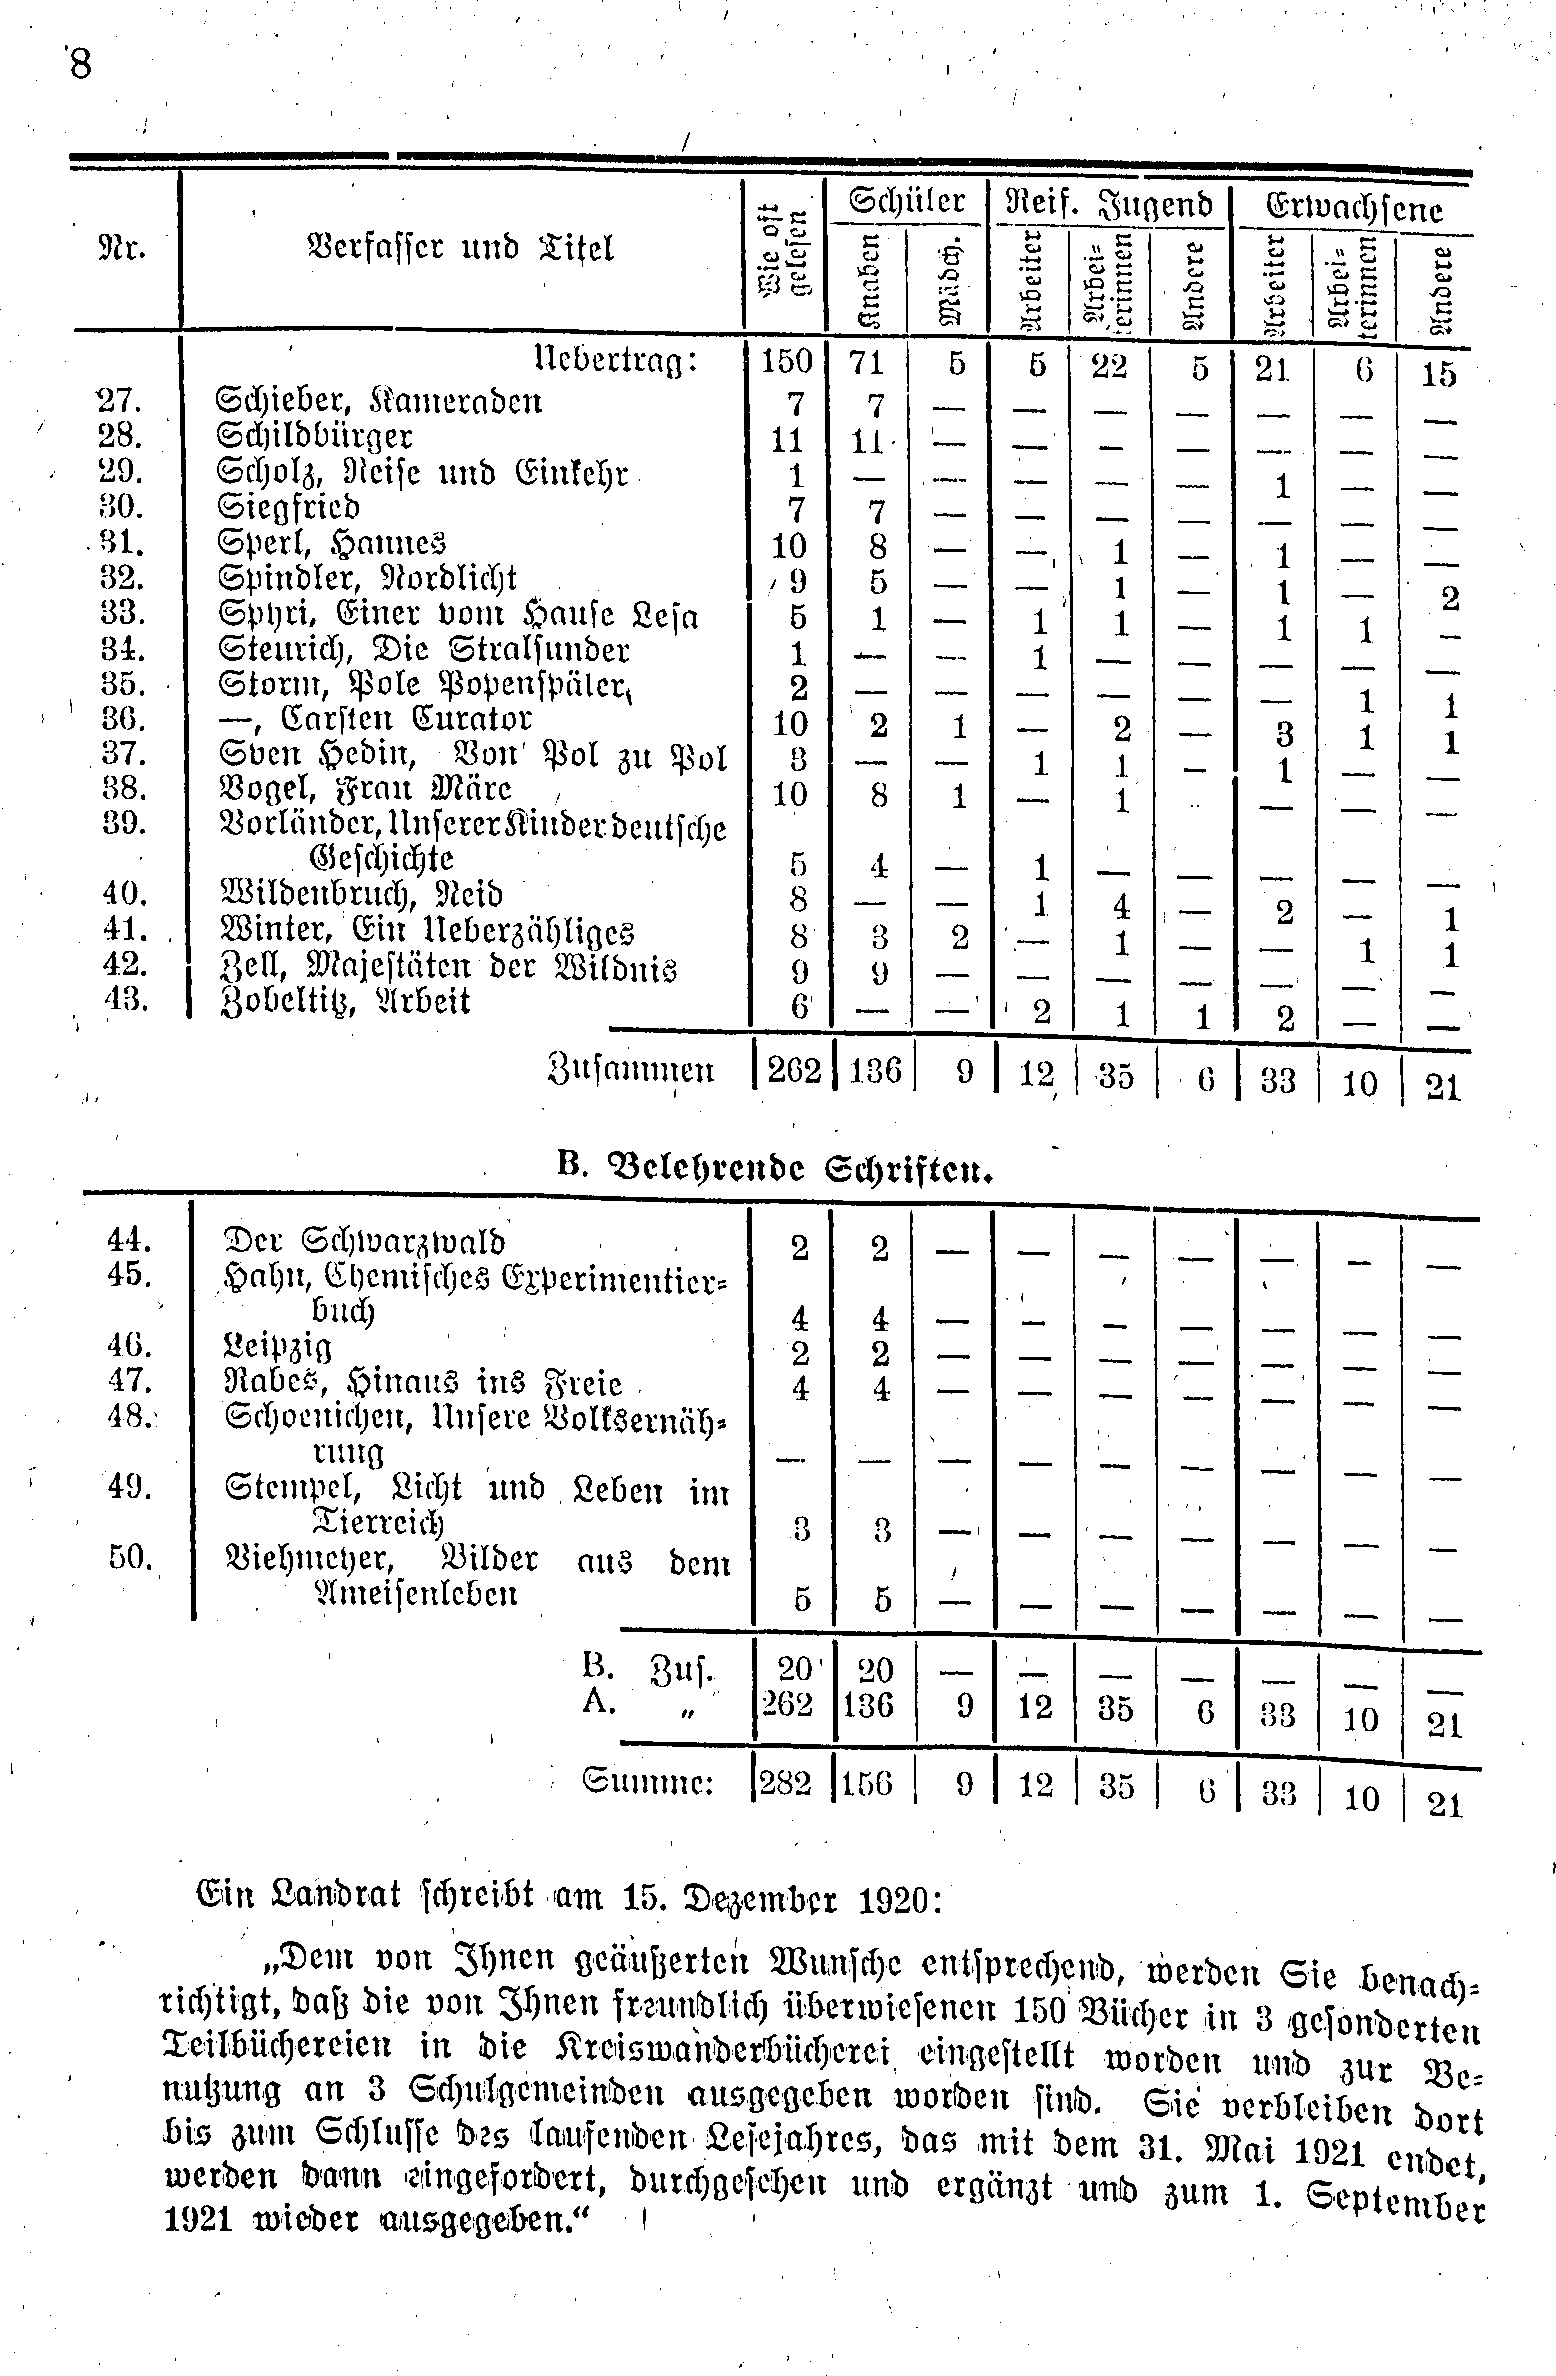
\includegraphics{img/scheffen_statistik_2.jpg}
\caption{Aus Scheffen 1921: 8.}
\end{figure}

Was sich in diesem Text auch findet, und dann die weiteren Texte des
Vereins prägen wird, ist die Behauptung, mit der eigenen Arbeit für «das
ringende Deutschtum» (Scheffen 1921: 9) unpolitisch zu sein. (Vergleiche
auch Weber 1929) Dies war, wie schon erwähnt, eine der
Grundüberzeugungen des völkischen Denkens:

\begin{quote}
«So will unser Verein durch seine Kulturarbeit ringendem Deutschtum ein
Helfer sein. Dabei stellt sich der Verein grundsätzlich außerhalb der
politischen Parteien und arbeitet interkonfessionell, wie es überhaupt
unsere Meinung ist, dass Kulturarbeit parteipolitisch und konfessionell
nicht gebunden sein darf, sondern das deutsche Geistesleben der
Vergangenheit und Gegenwart darzubieten hat.» (Scheffen 1921: 9)
\end{quote}

Zusätzlich zur Verschickung dieser Büchersammlungen und der Kontakte,
die zu halten versucht wurden, publizierte der Verein kontinuierlich
weitere Listen von Büchern (Hesse 1928) unterschiedlichen Umfangs und
für unterschiedliche -- wie man es heute nennen würde -- Zielgruppen.

1926 begann der Verein darüber hinaus «Grenzbüchereitagungen»
durchzuführen, die meist jährlich und meist in einem der deutschen
«Grenzgebiete» stattfanden. Auf diesen wurden die Arbeit des Vereins und
der Büchereien diskutiert, teilweise an weiteren Listen gearbeitet und
auch Büchereien besucht. Zudem wurden ab der zweiten Hälfte der 1920er
Jahre unregelmässig Lehrgänge angeboten. (Anonym 1926, Nachtigall 1929,
Hesse 1931) Ebenfalls zu dieser Zeit begann der Verein -- «in
Zusammenarbeit mit wissenschaftlichen Fach- und Forschungsstellen für
Grenz- und Auslandsdeutschtum, gefördert durch das Reichsministerium des
Innern» (Weber 1928: 27) -- «grenzwissenschaftliche Büchereien»
aufzubauen. Diese sollten, platziert in zentralen Orten im «Grenzland»,
dazu dienen, Wissen über die «Deutschtumsarbeit» zu verbreiten. (Weber
1928). Die Idee war, dass sich die in der Grenzlandarbeit tätigen
Personen in ihnen die Grundlagen für ihre Arbeit aneignen und aktuell
halten sollten.

Grundsätzlich verstand der Verein seine Arbeit selber nicht einfach als
das Verschicken von Büchern, sondern als «Bildungspflege». Wie ebenso
schon erwähnt, benannte sich der Verein 1928 explizit in
\emph{Grenzbüchereidienst und Bildungspflege e.V.} um. Unter diesem
Schlagwort wurde im gesamten Volksbildungswesen damals unter anderem die
explizite Arbeit an den Leser*innen -- also die Erziehung zum richtigen
Lesen -- verstanden. Dies bezog sich nicht nur auf Bücher und das Lesen,
sondern zum Beispiel auch auf das damals neue Medium Film (Ackerknecht
1918) sowie auf andere Bereiche, die man heute eher der Kulturarbeit
oder der sozialen Arbeit zuordnen würde. Scheffen umschreibt das
Verständnis dieses Begriffs durch den Verein wie folgt:

\begin{quote}
«{[}Man versteht{]} unter ‹Verbreitung› nicht nur -- wie vielfach nach
gegenwärtigem Sprachgebrauch in der Volksbildungspflege -- ein
mechanisches Hinauswerfen, sondern das Heranbringen guten Schrifttums an
weite Bevölkerungskreise, die sonst von dessen erzieherischer Wirkung
unberührt geblieben wären.» (Scheffen 1928b: 3)
\end{quote}

Damit bewegte sich der Verein auf Höhe des damaligen Verständnis von
Bildungspflege in Büchereien -- es ging um eine moderne, möglichst
effektive Organisation einer Büchereiarbeit, die auf bestimmte Ziele hin
ausgerichtet war. Der Verein verstand seine Büchereien als moderne
Einrichtungen.

\hypertarget{zusammenarbeit-mit-den-staatlichen-beratungsstellen}{%
\subsection{3.4 Zusammenarbeit mit den staatlichen
Beratungsstellen}\label{zusammenarbeit-mit-den-staatlichen-beratungsstellen}}

In den 1920er Jahren begannen also im DACH-Raum Gemeinden und der Staat
an sich mehr Verantwortung für die Volksbüchereien zu übernehmen. Einer
der Gründe dafür wird gewesen sein, dass sich die beiden 1918 neu
gegründeten Republiken neu aufstellten und sich dabei auch in anderen
Bereichen immer mehr engagierten. Das gesamte Bildungswesen (Pöggler
1974), aber zum Beispiel auch die soziale Infrastruktur, die öffentliche
Gesundheitspflege oder der Kulturbereich wurden immer mehr als
Aufgabenbereiche angesehen, in dem der Staat sich aktiv einbringen
müsse. All dies wurden Bereiche, die zum Teil der politischen
Verhandlungen wurden -- also für die Gesetze diskutiert und erlassen,
die Infrastrukturen aufgebaut, feste Etats in staatliche Budgets
eingestellt wurden und so weiter. (Allerdings war diese Entwicklung
zeitgleich auch in der Schweiz zu beobachten, die bekanntlich schon
länger, seit der Annahme der Bundesverfassung durch das Volk 1848, eine
Republik war.) Man kann dieses «Anwachsen der Staatsquote» als Teil der
Modernisierung der Gesellschaften im DACH-Raum interpretieren.

Im Büchereibereich schlug sich das zum Beispiel nieder in der Gründung
von staatlichen Beratungsstellen für das Volksbüchereiwesen sowie in
Diskussionen um ein Büchereigesetz. (Schuster 1929b) Für diese
Beratungsstellen gab es vor 1918 kaum Vorbilder, auch wenn Vorläufer in
der preussischen Provinz Oberschlesien (Kaisig 1912) sowie in Dänemark
bekannt waren. (Langfeldt 1924. 1931 wird dieser Vergleich zwischen
«Zentralbibliotheken» in Dänemark und Beratungsstellen in Deutschland
vom gleichen Autor (Langfeldt 1931: 234) auch explizit gezogen
werden.)\footnote{Die Arbeit in Oberschlesien war explizit im Rahmen der
  «Verdeutschungspolitik» Preussens gegenüber der polnisch sprechenden
  Bevölkerung in dieser Provinz eingebettet. Die Arbeit in Dänemark
  wurde in Deutschland als Teil einer vergleichbaren
  «Dänisierungspolitik» (Langfeldt 1924) interpretiert.} Sie wurden auch
nicht überall eingerichtet oder gar zentral von Berlin und Wien aus
organisiert. Vielmehr ergriffen einzelne Länder oder Provinzen die
Initiative, andere nicht. Zudem wurden die Beratungsstellen, die
eingerichtet wurden, offenbar unterschiedlich ausgestattet und wohl auch
mit unterschiedlichen Aufgaben betraut. Am Ende der 1920er Jahre gab es
in Deutschland dann so viele, dass sich 1929 auf der Jahrestagung des
\emph{Verbandes Deutscher Volksbibliothekare} eine
\emph{Arbeitsgemeinschaft Deutscher Beratungsstellenleiter} bildete.
(Schuster 1929b)\footnote{1938 liefert Franz Schriewer eine Monographie
  zu Aufgaben und Struktur der Beratungsstellen, bei ihm
  Volksbüchereistellen genannt, allerdings aus seiner spezifischen
  Perspektive und unter nationalsozialistischen Prämissen, also zum
  Beispiel nach dem «Führerprinzip» organisiert. Diese Schrift
  repräsentiert -- auch im Abschnitt zur Geschichte der Beratungsstellen
  (Schriewer 1938: 22--38) -- nicht die tatsächliche Situation während
  der Weimarer Republik.}

Aber grundsätzlich wurden die Beratungsstellen immer mit der
Unterstützung des Ausbaus des Büchereiwesens betraut. (Schriewer 1924a,
Schriewer 1925a, Schriewer 1938) Das heisst nicht, dass sie selber
Büchereien betrieben. Vielmehr scheinen sie akzeptiert zu haben, dass
diese von verschiedenen Vereinen mit teilweise unterschiedlichen Zielen
betrieben werden und dass deshalb die Positionierung einer Bücherei
gegenüber der jeweiligen Gemeinde sehr unterschiedlich sein konnte.
Gerade in Texten, die zu Beginn der nationalsozialistischen Herrschaft
geschrieben wurden, wird deshalb immer wieder erwähnt (und als negativ
dargestellt), dass es in der Zeit zuvor an vielen Orten mehrere
Büchereien auch unterschiedlicher politischer Ausrichtung gegeben hätte,
die erst jetzt (also im Nationalsozialismus) zentralisiert würden.
(Ruppe 1939) Die Beratungsstellen organisierten Statistiken, Beratungen
und Fortbildungen. (Siehe zum Beispiel Schriewer 1924a, Schriewer 1924c,
Schriewer 1925a) Oft betrieben sie auch «Wanderbüchereien», Sammlungen
von Büchern, die immer für mehrere Monate an eine Gemeinde oder einen
Verein abgegeben wurden und dann an einen anderen Ort weitergeschickt
wurden. Was diese Wanderbüchereien von heutigen Blockausleihen, die zum
Beispiel die \emph{Büchereizentrale Schleswig-Holstein} oder die
\emph{Stiftung Bibliomedia Schweiz} anbieten, unterscheidet, ist, dass
sie immer als Vorläufer einer «Standbibliothek» angesehen wurden
(Ackerknecht 1922) -- die Vereine oder Gemeinden sollten mit ihnen
praktisch lernen, eine Bücherei zu führen und dann in naher Zukunft
selber eine solche gründen.

In diesen Beratungsstellen wurden, finanziert von den Provinzen und
Ländern, feste Stellen geschaffen, also in gewisser Weise
Karrieremöglichkeiten für Personen, die zu Expert*innen im Büchereiwesen
wurden, eingerichtet. Gleichzeitig erreichten diese Beratungsstellen
wohl nie alle Büchereien. Es gab zum Beispiel die gesamte Zeit über
sowohl für die katholischen Büchereien als auch die Arbeiterbibliotheken
eigene, den Beratungsstellen vergleichbare Strukturen, die wohl die
jeweils betreffenden Büchereien besser organisierten. Die staatlichen
Beratungsstellen scheinen teilweise mit ihnen zusammengearbeitet zu
haben, aber man darf sich diese Koordination wohl nicht so relativ
problemlos vorstellen, wie dies heute zwischen den jeweiligen
Nachfolgeeinrichtungen (also staatlichen Beratungsstellen, deutschem und
österreichischen \emph{Borromäusverein} beziehungsweise \emph{Sankt
Michaelsbund} in Bayern) der Fall ist.

Relevant für die Geschichte der Grenzbüchereiarbeit ist nun, dass eine
ganze Anzahl von Personen aus diesen Beratungsstellen aus den
«Grenzgebieten» mit dem Verein zusammenarbeitete oder aber explizit im
Verein aktiv war. Prominentestes Beispiel dafür ist wieder Franz
Schriewer, der für den Verein aktiv war, aber gleichzeitig bis 1933 die
\emph{Zentrale für Nordmarkbüchereien} in Flensburg leitete. Er war
keine Ausnahme. Vielmehr war der Verein eng mit den Beratungsstellen,
aber auch den betreffenden Ministerien vernetzt. Immer wieder traten
Leiter von Beratungsstellen auf den Tagungen des Vereins auf, wurden
Arbeitsberichte der Beratungsstellen vom Verein publiziert (vergleiche
zum Beispiel Fischer 1928) und wurde gleichzeitig von den
Beratungsstellen auf die Arbeit des Vereins zurückgegriffen.

Auffällig ist, dass in den Darstellungen des Vereins die Arbeit der
Beratungsstellen, der Büchereien vor Ort und des Vereins als eine
Gesamtheit dargestellt werden. Alle Büchereien, die in bestimmten
Gebieten eingerichtet wurden, wurden offenbar zur «Grenzbücherei»
erklärt, solange sie nur einen Kontakt zu den Beratungsstellen oder dem
Verein hatten. (Scheffen 1928a) Ob die Bibliothekar*innen vor Ort oder
deren Trägereinrichtungen dies auch so sahen, oder ob sie andere Ziele
hatten, schien dabei nicht von Interesse zu sein.

Dies wird vor allem dann deutlich, wenn diese Denkweise auf andere
Länder übertragen wird. Gerade Dänemark und der Tschechoslowakei wird
explizit unterstellt, dass ihre jeweilige Bibliothekspolitik darauf
ausgerichtet sei, dass jeweils ein Volk (das Dänische und das
Tschechische) eine Vorherrschaft im jeweiligen Land etablieren solle. In
beiden Ländern waren Bibliotheksgesetze erlassen worden, welche für eine
Versorgung der Bevölkerung mit Büchereien sorgen sollten.\footnote{Auch
  Belgien hatte ein Bibliotheksgesetz erlassen, das von Scheffen (1928:
  12) aber nur kurz -- weil seiner Meinung nach noch nicht wirklich
  wirksam -- erwähnt wird. Das polnische Büchereiwesen bewertet Scheffen
  ebenfalls unter völkischem Gesichtspunkt: «Das polnische Büchereiwesen
  ist noch unterentwickelt, aber mit starken nationalem Machtinstinkt
  und rücksichtlosem Willen wird hier versucht, zugleich mit der
  Polnisierung der dem polnischen Staat zugefallenen deutschen
  Minderheiten auch eine Einwirkung auf politisch deutsch gebliebenes
  Gebiet zu erzielen. Die slawischen Dialekte der oberschlesischen und
  kaschubischen Bevölkerung wie auch die sprachlich nicht deutschen
  Masuren gaben den Polen den Vorwand zu dem Versuch, hier innerhalb
  unserer jetzigen deutschen Reichsgrenzen völkisch-politischen Einfluß
  zu gewinnen.» (Scheffen 1928a: 12)} Wilhelm Scheffen (1928) diskutiert
diese explizit als Gefahr. Das tschechoslowakische Gesetz wird (in
Auszügen aus der deutschen Version) sogar in den Mitteilungen
abgedruckt. (Tschechoslowakei 1928) Dabei war dieses Gesetz explizit so
ausgestaltet worden, dass alle nationalen Minderheiten, also auch die
deutschsprachige, ihre eigenen Büchereien haben sollten.
(Tschechoslowakei 1928: 23--24, Moucha 1929) Überall, wo 400 oder mehr
Angehörige einer Minderheit lebten, war eine eigene Büchersammlung
einzurichten. Waren es weniger, so wurden Büchereien in naheliegenden
Gemeinden eingerichtet. Sicherlich kann man sich heute fragen, warum die
Büchereien überhaupt nach sprachlichen Minderheiten getrennt werden
mussten. Aber, wenn es dem \emph{Grenzbüchereidienst} nur darum gegangen
wäre, dass die deutsche Sprache oder Kultur gefördert wird, dann hätten
sie das Gesetz als Vorbild ansehen können -- aber durch das völkische
Denken wurde es vor allem als Gefahr interpretiert. Scheffen (1928: 11)
diskutiert vor allem, was diese Regelung für «deutsche Gemeinden»
bedeuten würde, in denen auch «Tschechen» wohnen. Aus den Reihen des
Vereins wird später ein Büchereigesetz vor allem deshalb gefordert
werden, um die gleichen Werkzeuge im «Volkskampf» zur Verfügung zu
haben, wie die Staaten um Deutschland herum sie hätten. (Schriewer
1933b)

Was aus den Veröffentlichungen des Vereins nicht ersichtlich wird, ist,
wie dieser überhaupt seine Aktivitäten finanzierte. Gerade der Erwerb
und die kostenlose Versendung von Büchern bedurfte eines
kontinuierlichen Geldflusses. Wie gesagt war der Verein offenbar immer
gut mit den jeweiligen gesellschaftlichen Eliten verbunden. Seine
Verbindungen zu staatlichen Beratungsstellen oder auch Ministerien (die
mehrfach bei den Tagungsberichten dankend erwähnt werden) lassen
zumindest vermuten, dass ein Teil dieser Mittel auch direkt aus
staatlichen Quellen stammte.

\hypertarget{grenzbuxfcchereiarbeit-wuxe4hrend-des-nationalsozialismus}{%
\section{4. Grenzbüchereiarbeit während des
Nationalsozialismus}\label{grenzbuxfcchereiarbeit-wuxe4hrend-des-nationalsozialismus}}

\hypertarget{existenz-nach-der-nationalsozialistischen-machtergreifung}{%
\subsection{4.1 Existenz nach der nationalsozialistischen
Machtergreifung}\label{existenz-nach-der-nationalsozialistischen-machtergreifung}}

Das übergreifende Verhalten des deutschen Volksbüchereiwesens im
Nationalsozialismus ist als Selbstanpassung beschrieben worden. (Andrae
1970, Kettel 1981, Boese 1987, Vodosek \& Komoroski 1989, Vodosek \&
Komoroski 1992, Schmitz \& Knoche 2011, Kuttner \& Vodosek 2017) Sowohl
Verbände, Infrastruktureinrichtungen wie die Fachstellen und Büchereien
als auch Bibliothekar*innen selbst passten sich schnell dem neuen System
an. Jüdische und politisch unliebsame Kolleg*innen wurden schnell
ausgeschlossen. Der \emph{Verband Deutscher Volksbibliothekare} wurde
direkt in das nationalsozialistische System integriert. Im Rahmen der
«Gleichschaltung» wurden bislang führende Personen teilweise in die
zweite Reihe gestellt -- wenn auch nicht unbedingt für lange -- und
beispielsweise die Zeitschriften \emph{Bücherei und Bildungspflege} und
\emph{Hefte für Büchereiwesen} 1933 beendet, die Redaktionen entlassen
und dafür die Zeitschrift \emph{Die Bücherei} gegründet, welche mit
einer neuen Redaktion, aufgebaut nach dem Führerprinzip, herausgegeben
wurde. Gleichwohl geschah diese Übernahme in gewisser Weise geordnet.
(Fritz, Ackerknecht \& Schuster 1933, Schuster 1934) Gleichzeitig war
die gesamte Bücherei- und Literaturpolitik des Nationalsozialismus durch
interne Kämpfe zwischen verschiedenen Organisationen und unklaren
Richtlinien gekennzeichnet, innerhalb derer sich alle Beteiligten
ständig neu orientieren mussten. (Barbian 2010)

Vor diesem Hintergrund ist es hervorhebenswert, dass dies alles für den
Verein \emph{Grenzbüchereidienst und Bildungspflege e.V.} nicht galt. Er
wurde weder verboten noch gleichgeschaltet, sondern konnte die gesamte
Zeit des Nationalsozialismus weiter existieren. Einzig sein Name wurde
reduziert zu \emph{Grenzbüchereidienst e.V.} (Scheffen 1933) Einzelne
Vertreter hatten im Rahmen der internen Machtkämpfe im
Nationalsozialismus Rückschläge zu erfahren, allerdings auch in Massen.
Das prominente Beispiel ist hier wieder Franz Schriewer, der 1933 seine
Stelle in Flensburg verlor. Dietmar Albrecht schreibt im
«Biographische{[}n{]} Lexikon für Schleswig-Holstein und Lübeck», dass
er «Politischen Denunziationen und ehrverletzenden Beschuldigungen»
(Albrecht 2020 {[}1987{]}: 2442) ausgesetzt gewesen wäre, führt aber
nicht weiter aus, worum es genau ging. Danker (2017) geht, aufgrund
vorliegender Dokumente, etwas tiefer auf diese Auseinandersetzungen ein,
wertet sie aber als Form der eher persönlichen Auseinandersetzungen, die
am Anfang des nationalsozialistischen Regimes in gewisser Weise «normal»
waren: «Man hatte {[}Schriewer{]} förmlich aus der Region gejagt; eine
gewiss sehr, sehr bitterer Erfahrung. Aber Ärger mit lokalen NS-Größen
sagt wenig über Nähe oder Distanz zur NS-Bewegung und zum neuen Staat
aus. Das gilt insbesondere für Stadt und Landkreis Flensburg, wo
regionale NS-Repräsentanten für viel Kabale und Konflikte standen, eine
sehr aufgeregte Minderheiten- und Grenzpolitik des Jahres 1933 ihr
Übriges leistete.» (Danker 2017: 87f.) Dafür wurde Schriewer 1934
Stadtbibliothekar in Frankfurt/Oder und betrieb dann dort weiter
«Grenzbüchereiarbeit», indem er das Büchereisystem in der dortigen
«Grenzregion» organisierte. (Schriewer 1934) Für einige Jahre war er
dann in Berlin als Leiter der \emph{Reichsstelle für das
Volksbüchereiwesen} des \emph{Reichsministeriums für Wissenschaft,
Erziehung und Volksbildung} tätig, bevor er 1937 nach Frankfurt
zurückkehrte. Während seiner Zeit in Berlin war er auch Herausgeber von
\emph{Die Bücherei} und insoweit einer der einflussreichsten Personen im
deutschen Volksbüchereiwesen der damaligen Zeit. Er erlebte 1933 also
einen kurzen, persönlichen Tiefpunkt, dem aber recht bald ein
Karrieresprung folgte.

Der Verein selbst wurde aktiv in das nationalsozialistische
Büchereiwesen integriert. Die gerade erwähnte Fachzeitschrift \emph{Die
Bücherei} wurde als Publikationsorgan des Vereins genutzt (Fritz,
Ackermann \& Schuster 1933), was auch explizit im Impressum vermerkt
wurde. Deshalb erschienen in ihr, noch regelmässiger als zuvor in der
\emph{Bücherei und Bildungspflege}, Beiträge zum «Grenzbüchereidienst».
Nach 1934 -- einem Jahr, in welchem sowohl Franz Schriewer (Schriewer
1934) als auch Wilhelm Scheffen (Scheffen 1934) noch je eine längere
Darstellungen zur Grenzbüchereiarbeit, jetzt als Teil der staatlichen
Büchereiplanungen, veröffentlichten -- handelte es sich dabei aber vor
allem um Berichte zu Treffen des Vereins (beispielsweise Hesse 1937,
Zweck 1937). Inhaltlich tiefergehende Artikel wurden weiterhin vor allem
in den \emph{Mitteilungen} publiziert. Die einzige Ausnahme davon bietet
eine 1940 in \emph{Die Bibliothek} veröffentlichte historische Übersicht
zum Grenzbüchereidienst, wieder von Wilhelm Scheffen (Scheffen 1940). In
dieser stellt er die Arbeit des Vereins auch vor 1933 als
übereinstimmend mit den Zielen des Nationalsozialismus dar -- eine
Position, mit der er, wie gleich im nächsten Abschnitt sichtbar werden
wird, nicht alleine stand.

Ein Unterschied war, dass der Verein jetzt, nach 1933, weniger ein
Monopol auf das Thema völkische Büchereiarbeit hatte. Stattdessen wurden
gerade von nationalsozialistischen Aktiven im Büchereiwesen die Themen
des Vereins aufgegriffen und inhaltlich ausgedehnt. Ein Beispiel dafür
ist ein ebenfalls in \emph{Die Bücherei} erschienener Text zu Büchereien
«jenseits der Reichsgrenze». (Roscher 1934) In ihm werden Diskurse, die
bislang in den \emph{Mitteilungen} gepflegt wurden, erweitert. Sie
verändern sich damit, aber es zeigt sich auch, dass diese Erweiterung in
Richtung explizit nationalsozialistischer Ideologie einfach, und ohne
dabei Widersprüche zu produzieren, möglich war. Der Autor nimmt quasi
das völkische Denken, dass sich im Verein geographisch immer um die
sogenannten «Grenzgebiete» gedreht hatte, und erweitert es -- im Text
erst geht es nur um diese Gebiete, dann aber auch um «das Deutschtum» im
gesamten Europa sowie der Sowjetunion und am Ende um jenes, dass er
weltweit verortet, namentlich in der damaligen britischen Kolonie
Südafrika und bei deutschen Gemeinschaften in Südamerika. Für den Autor
gelten jetzt alle Menschen, die irgendwelche deutschen Vorfahren haben,
als «Deutsche», deren Volkstum gefährdet sei. Zudem verbindet er das
völkische Denken, welches im Verein betrieben wurde, explizit mit
antisemitischem Denken. Dies zeigt sich im folgenden Zitat, dass sich am
Beginn nicht gross anders liest, als der weiter oben zitierte, 1929 in
den \emph{Mitteilungen} publizierte völkische Grundlagentext (König
1929), bevor es dann explizit antisemitisch wird.

\begin{quote}
«Wir müssen uns immer wieder ins Bewußtsein rufen: Über ein Drittel
aller Deutschen lebt außerhalb des Deutschen Reiches, verteilt auf vier
weitere deutsche Staaten (Österreich und Danzig, Luxemburg und
Liechtenstein), einen Staat mit deutscher Mehrheit (Schweiz) und 29
andere Staaten mit geschlossenen deutschen Siedlungsgruppen, ferner auf
das Streudeutschtum in sämtlichen Ländern der Erde {[}\ldots{]}.
Demgemäß ist auch das deutsche Büchereiwesen jenseits der Reichsgrenze
zahlenmäßig beachtlich und vor allem: sehr mannigfachig. {[}...{]}

Überall auf der Erde, wo deutsches Volkstum mit fremden zusammenstößt,
ohne von einer starken Reichsgewalt geschützt zu werden, ist das
Deutschtum gezwungen, sich zu behaupten, Sprache und Kultur zu
verteidigen und den Abfall deutscher Volksgenossen vom angestammten Sein
zu verhindern. Das gilt auch von {[}sic!{]} Staaten, wie Luxemburg oder
der Schweiz, die ganz oder vorwiegend deutschen Volkstums sind und die
doch mehr oder weniger (die gemischtvölkische Schweiz weniger) unter
französischem Einfluß stehen. Das gilt auch von {[}sic!{]} Österreich,
wo das Judentum auf vielen Lebensgebieten noch unumschränkte Macht hat.»
(Roscher 1934: 537)
\end{quote}

Weiterhin beschreibt der Autor die Notwendigkeit, die Büchereien, die er
zum «Auslandsdeutschtum» zählt, und deren Bestände er beispielsweise als
teilweise gefährlich undeutsch beschreibt (weil sie in Dänemark auch
Literatur enthielten, die im Deutschen Reich verboten worden war, oder
weil sie in Südafrika auch englische «Groschenhefte» umfassen würden),
nicht nur zu beraten oder zu unterstützen, sondern -- kongruent mit der
Vorstellung einer gleichgeschalteten und autoritär geführten
Gesellschaft -- explizit vom Deutschen Reich aus anzuleiten.

In gewisser Weise wurden Vorstellungen, die der Verein vor 1933
vertreten hatte, im Nationalsozialismus also aufgegriffen, radikalisiert
und als Teil der staatlichen Aufgaben begriffen.\footnote{Ob sich dies
  dann auch in der realen Büchereiarbeit niederschlug, ist eine offene
  Frage. Barbian (2010) zeigt, dass die reale Bücherei- und
  Literaturpolitik, wie andere Bereiche des nationalsozialistischen
  Staates auch, von ständigen Machtkämpfen zwischen verschiedenen
  Einrichtungen mit jeweils umfassenden Machtanspruch gekennzeichnet
  waren, die zu widersprüchlichen Realitäten in der Praxis führten.
  Insoweit ist das auch hier zu vermuten.}

\hypertarget{grenzbuxfcchereifahrten-und-selbstanpassung}{%
\subsection{4.2 Grenzbüchereifahrten und
Selbstanpassung}\label{grenzbuxfcchereifahrten-und-selbstanpassung}}

Grundsätzlich wurden Verein und Aktive der Grenzbüchereiarbeit also
recht problemlos in das nationalsozialistische System integriert. Die
Ausgaben der \emph{Mitteilungen}, die in dieser Zeit erschienen, zeigen,
dass sich dafür die Ideen und Arbeitsweisen nicht ändern mussten.
Vielmehr wurden sie nur leicht in der Terminologie angepasst und die
Verbindung zum Staat scheint noch enger geworden zu sein. Sichtbar wird
dies beispielsweise in einer noch besseren Ausstattung der
\emph{Mitteilungen} selbst. Sie enthalten in dieser Zeit mehr Graphiken,
ein besseres Druckbild oder auch besseres Papier. Aber es ändert sich
zum Beispiel kaum, wer oft in ihnen publiziert. Einzig, dass neben
Wilhelm Scheffen jetzt auch seine Ehefrau Luise Scheffen-Döring
verstärkt auftrat, war neu.

Aus den Tagungen des Vereins werden nun «Grenzbüchereifahrten».
(Scheffen-Döring 1935, Anonym 1936, Scheffen-Döring 1936,
Scheffen-Döring 1938, Scheffen-Döring 1939a, Scheffen-Döring 1939b,
Heiligenstaedt 1939) Diese führten immer rund eine Woche lang in ein
Grenzgebiet. Dort wurden weiterhin Vorträge geboten, aber auch Besuche
in kleinen Büchereien und Besuche der Grenze selbst, von der aus dann
jeweils gemeinsam in angeblich deutsches Land geschaut wurde, das jetzt
zum falschen Staat gehören würde. Zumindest in den dazugehörigen
Berichten wird immer ein Blick in ein Feindesland inszeniert und diesem
«Feind» jeweils unterstellt, das Land nicht richtig zu
nutzen.\footnote{Ein Beispiel: «Der Nachmittag gehört dem Kreise
  Groß-Wartenberg, wo Kreissparkassendirektor Kellner uns die Grenze
  entlangführt. Hier tritt ein wenig bekanntes und doch besonders großes
  Unrecht von Versailles in die {[}sic!{]} Erscheinung: ohne Abstimmung,
  ohne irgend eine historische Grundlage, hat man hier 90 Gemeinden und
  Güter mit über 26 000 Menschen und 51 000 Hektar Land an Polen
  gegeben. {[}\ldots{]} Die Barriere mitten über die Landstraße, der wir
  noch auf mehrere Meter fernbleiben müssen, zeigt uns die ganze
  Sinnlosigkeit dieser Landzerreißung.\\
  Was ist der tiefere Grund? Auch Herr von Heinersdorf, der
  alteingesessene Landrat des Kreises, der die ganzen Kampfjahre
  miterlebt hat, kann ihn uns nicht nennen. Sind auch seit der
  Jahrhundertwende gelegentlich einige polnische Ansprüche erhoben
  worden, so hat man doch {[}vor 1921{]} nicht einmal daran gedacht,
  einen polnischen Zählkandidaten aufzustellen. Wirtschaftliche Vorteile
  hat der neue Landbesitz Polen nicht gebracht, die Verwaltung dieses
  dünnbesiedelten Agrarlandes ist teuer, der Weg zu nächsten Kreisstadt
  Ostrovo 35 Kilometer weit, also praktisch zum Absatz unbenutzbar. Auch
  strategisch hat das Gebiet keine Bedeutung, es bleibt als einzige
  Lösung die mechanische Zugrundelegung der gefälschte Spettschen
  Nationalitäten-Karte, die bei so mancher Entscheidung von Versailles
  für den Osten eine verhängnisvolle Rolle gespielt hat.»
  (Scheffen-Döring 1935: 20--21)\\
  Die Autorin dieser Zeilen verschweigt die, teilweise bewaffneten und
  sehr wohl bekannten, Auseinandersetzungen zwischen Polen und
  Deutschland kurz nach dem Ende des Ersten Weltkriegs (zumeist erster,
  zweiter und dritter polnischer Aufstand genannt) sowie die Ergebnisse
  einer Volksabstimmung, die zur Teilung der ehemaligen Provinz
  Oberschlesien führten. Da diese Auseinandersetzungen, insbesondere die
  «Schlacht am Annaberg» im Mai 1921, zu den ständig wiederholten
  Geschichten der völkischen Bewegung gehörten, kann man davon ausgehen,
  dass das nicht unabsichtlich geschah. (Siehe auch die Berichte aus
  allen «deutschen» Volksbüchereien, die nach diesem dritten polnischen
  Aufstand in der Zeitschrift \emph{Die Volksbücherei in Oberschlesien}
  publiziert wurden und teilweise von Schliessungen oder Zerstörungen in
  den Büchereien berichteten. (Verband oberschlesischer Volksbüchereien
  E.V. 1921))} Und gleichzeitig werden Büchereien als Teil eines Kampfes
zwischen Völkern dargestellt, beispielsweise im Abschnitt «Das Buch im
Grenzkampf» im Bericht der «Bayerischen Ostmarkfahrt» 1936
(Scheffen-Döring 1936: 48--53) oder aber, wenn Josef Wuß, «Leiter der
Staatlichen Grenzbüchereistelle, Bayreuth, und der Gaubüchereistelle des
NSDAP», in den Mitteilungen das Ziel seiner Stelle wie folgt umschreibt
(vergleiche auch Taupitz 1938):

\begin{quote}
«Der Nationalsozialismus will den deutschen Menschen entsprechend seinem
ihm vorschwebenden Ideal führen und formen. Dieser Erziehungs- und
Bildungsarbeit hat sich die Volksbücherei ein- und unterzuordnen. Sie
ist als volksnahe und von Staats wegen fachlich richtig geführte
Vermittlungsstelle notwendiger und wichtiger Bücher verpflichtet und in
der Lage, die Formung des inneren Menschen im Sinne des
Nationalsozialismus zu unterstützen. Indem sie das Schrifttum der Nation
in führender und leserpsychologischer Auswahl bereithält, wirkt sie
zugleich dem reinen Intellektualismus entgegen, der ja immer im Schatten
der Bücherwelt steht.» (Wuß 1936: 63)
\end{quote}

Wuß bewegt sich mit dieser Darstellung weiter im Diskursrahmen der
Büchereipädagogik. (Der Begriff «Leserpsychologie» wurde gemeinhin
benutzt, wenn es darum ging, zu verstehen, wie und warum einzelne
Menschen lesen.) Verändert hat sich also nicht die eigentliche Arbeit
des Vereins, es wird jetzt nur statt völkischer explizit einer
nationalsozialistischen Denkweise gefolgt.

Dies zeigt sich gut in einer der beiden Ausgaben der
\emph{Mitteilungen}, die direkt 1933 erschienen. Diese Ausgabe besteht
aus nur zwei Artikeln (Scheffen 1933, Schriewer 1933b) und einer Karte.
Im einleitenden Text behauptet Scheffen zwar -- wie dies auch
vergleichbare Texte anderer Organisationen taten, welche versuchten,
1933 für sich einen Platz im nationalsozialistischen System zu finden --
zuerst folgendes: «Ein Sturmwind ist über Deutschland dahingerauft. Ein
neues Deutschland ist geworden. Die Entwicklung geht, wohin wir blicken,
gewaltig schnell weiter.» (Scheffen 1933: 3). Anschliessend stellt er
aber die Arbeit des Vereins vor allem als kontinuierlich dar. Schon
lange wäre dieser von der «Deutschtumsabteilung des Reichsministerium
des Inneren {[}...{]} wesentlich gefördert {[}worden{]}» (Scheffen 1933:
4). Er schreibt von 2000 betreuten Büchereien und rund 100
grenzwissenschaftlichen Büchereien, die der Verein direkt unterhält,
sowie von alleine in den ersten neun Monaten 1933 verschickten 33.956
Büchern (Scheffen 1933: 5). Ebenso erwähnt er eine weitere
«Grundbestandsliste», die der Verein gerade erstellt hatte. Seine
Vorstellung von der zukünftigen Aufgabe des Vereins liest sich nicht
wirklich anders, als vor der nationalsozialistischen Machtübernahme:

\begin{quote}
«Bei der Gewinnung unseres ganzen Volkes für die Idee der Sendung des
deutschen Menschen im Schicksalsland des Ostens, bei der Stützung des
Grenzländers in seiner Pionierarbeit und bei der Pflege der organischen
Einheit von dieseits und jenseits der Grenze wird überall das deutsche
Buch mit großen Wirkungsmöglichkeiten einzusetzen sein.» (Scheffen 1933:
6)
\end{quote}

Interessant ist die Selbstdarstellung des Vereins auf der dieser Ausgabe
der \emph{Mitteilungen} beigefügten Karte. Diese zeigt die Grenzen des
damaligen Deutschen Reiches, dann die «abgetretenen Gebiete», also die
durch den Versailler Vertrag und teilweise daran anschliessende
Volksabstimmungen an andere Länder abgetretenen Gebiete. Hier werden
sie, indem «die früheren Reichsgrenzen» eingetragen werden, als
gewissermassen dem Deutschen Reich zugehörig gekennzeichnet.\footnote{Obgleich
  viele von ihnen selber erst wenige Jahrzehnte vor oder bei der
  Reichsgründung 1871 durch Kriege Teil deutscher Staaten geworden waren
  (Elsass-Lothringen, Schleswig).} Zudem eingetragen sind auf der Karte
die «Grenzbüchereigebiete», in denen der Verein tätig war. Diese folgen
fast genau den völkischen Vorstellungen, die in dem weiter oben
zitierten Text von König (1929) dargestellt wurden: Sie liegen an allen
Grenzgebieten des Deutschen Reiches (zu Dänemark, Polen, der
Tschechoslowakei, Frankreich, Luxemburg und Belgien), ausser denen, die
König als Deutsch (oder «westgermanisches Sondervolk») beschreibt (also
Schweiz, Österreich, die Niederlande sowie den Teil der
Tschechoslowakei, der wohl als «Deutsch» galt). Dass die Grenze zur
Freien Stadt Danzig auch als «Grenzbüchereigebiet» gilt, liegt wohl
daran, dass sie selbst direkt an Polen grenzt. (Insoweit stimmt nur die
Grenze zu Luxemburg nicht mit Königs Aufzählung überein.) Weiterhin sind
die «Büchereizentralen» (also die staatlichen Beratungsstellen)
eingezeichnet, welche in diesen «Gebieten» tätig sind. Sie alle sind
jeweils mit einer Linie mit dem Vereinssitz in Berlin verbunden. Es
entsteht so der Eindruck, als würde der Verein den Anspruch erheben,
diese Beratungsstellen -- in der zeitgenössischen Terminologie -- zu
führen.

\begin{figure}
\centering
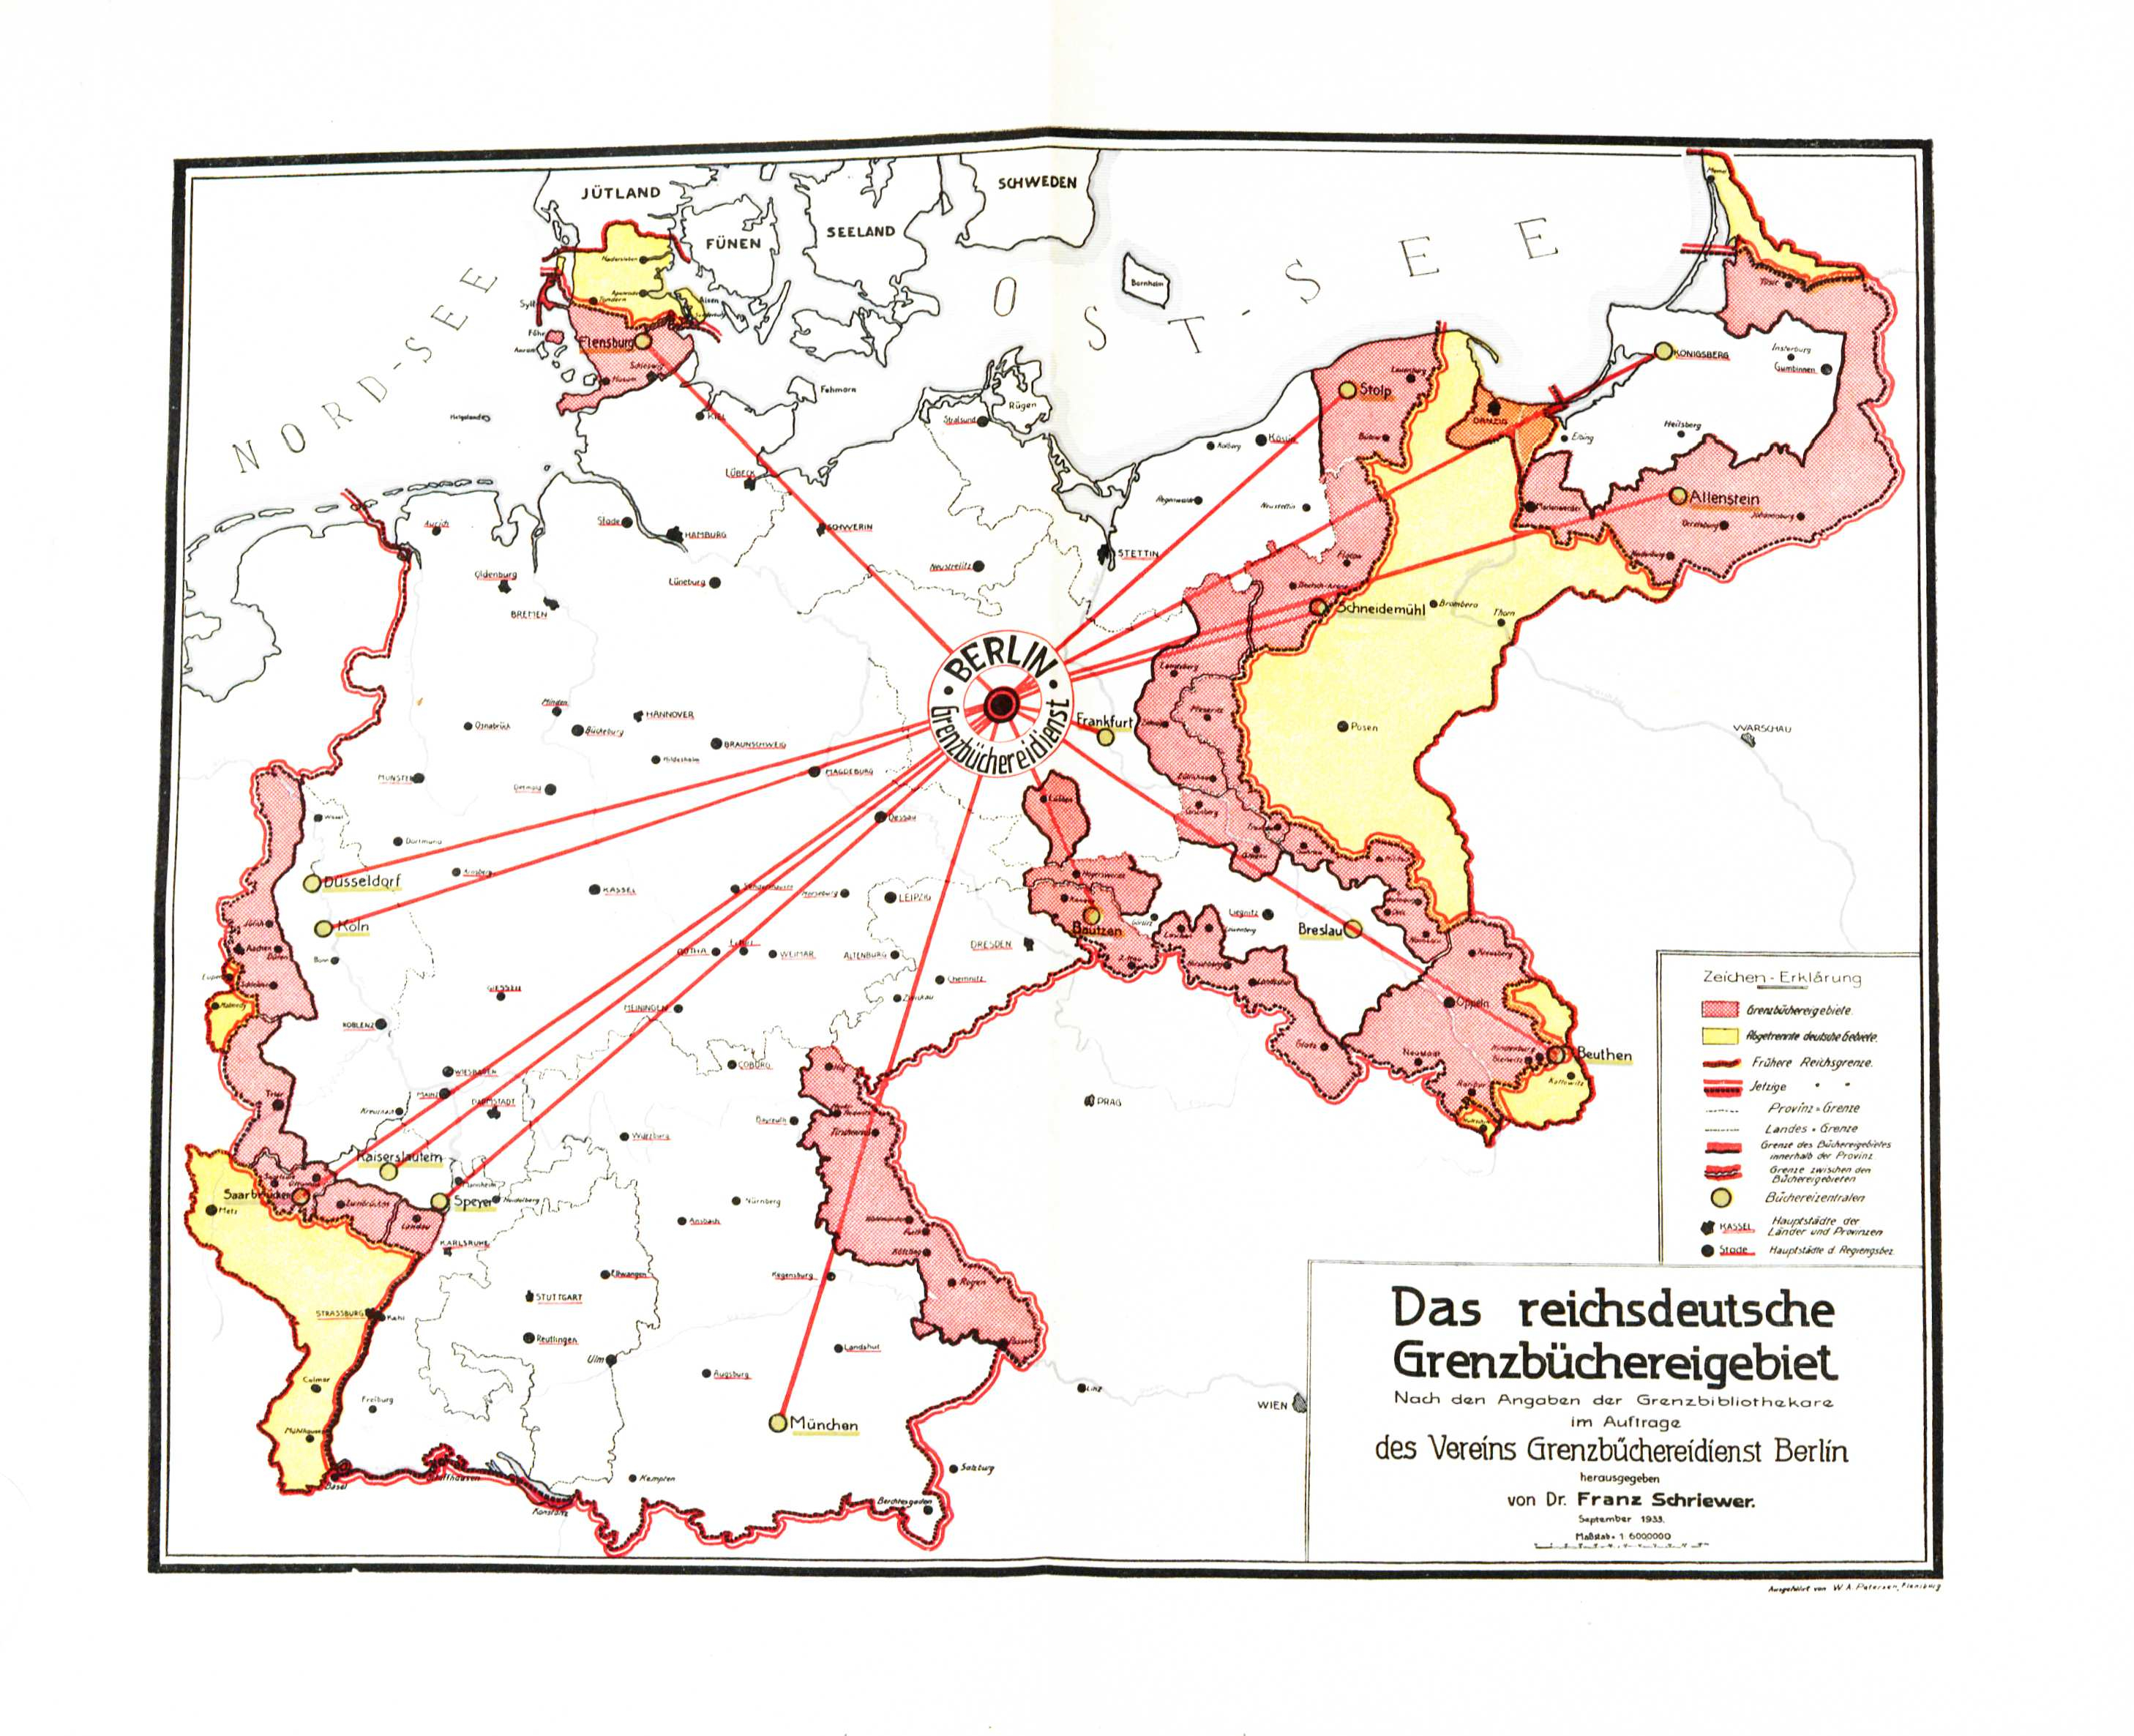
\includegraphics{img/karte_reichsdeutsche.jpg}
\caption{Karte aus Grenzbüchereidienst e.V. Mitteilungen (1933) 12:
Umschlagseite.}
\end{figure}

Der zweite Text von Franz Schriewer führt diese Selbstdarstellung zu
politischen Forderungen weiter. In einem Schritt führt Schriewer den bis
dato noch etwas offenen Volksbegriff, der in den \emph{Mitteilungen}
verwendete wurde, direkt mit der nationalsozialistischen Vorstellung
zusammen:

\begin{quote}
«{[}Es{]} heißt für unsere Büchereiarbeit: Alles, was in unserem
Schrifttum, besonders in der Schönen Literatur, abgestandene Romantik
oder museale Beschreibung von Volkstumserscheinungen ist, ist unwirksam
und kann entbehrt werden. Wenn wir eine neue Bodenverbundenheit des
deutschen Menschen wollen, genügt uns nicht eine leere Heimatpflege. Es
hilft uns auch nicht der künstliche Mythos. Wir müssen zurück zu den
wirklichen Kräften und dürfen nicht an gewesenen Formen hängenbleiben.
Volkstum ist nicht starre Form und ewig verharrende Erscheinung,
Volkstum ist ein geistig-seelisches Gerichtetsein aus Schicksal, Blut
und Rasse.» (Schriewer 1933b: 11f.)
\end{quote}

Weiterhin beschreibt Schriewer die bisherige Arbeit des Verein als
unpolitisch und über den Parteien stehend, wie dies im völkischen
Diskurs -- wie weiter oben geschildert -- normal war. Jetzt nennt er
dies aber explizit eine Strategie, um in der Weimarer Demokratie
überhaupt völkische Politik betreiben zu können. Egal, ob dies von
Schriewer (oder anderen Aktiven) während der Weimarer Republik
tatsächlich so gesehen wurde, bestätigt er hiermit, dass auch völkische
Aktiven zumindest im Nationalsozialismus klar ist, dass ihre Haltung
sehr wohl politisch war -- auch wenn sie immer behauptet hatten, mit
«dem Volk» eine überzeitliche Entität zu unterstützen. Schriewer
schreibt:

\begin{quote}
«Unser Verhältnis zum Staat wird damit {[}mit der
nationalsozialistischen Machtergreifung{]} heute ein grundlegend
anderes. Wir haben all die Jahre bewußt unsere Kulturarbeit an den
Grenzen abseits gehalten vom Parteienstaat. Wir trieben Kulturpolitik,
klammerten aber stillschweigend das Wort ‹Politik› ein. Indem wir uns
auf die Insel der Volkstumspflege zurückzogen, entpolitisierten wir
gleichsam unsere Arbeit. War das Mangel an politischem Gefühl oder
Verkennung der Tatsache, dass die Politik den Vorrang im Schicksal eines
Volkes hat, war das ein Nachwirken bürgerlich-ästhetisierenden
Bildungsbetriebes? Nein, wir handelten so, wenn vielleicht auch nicht
immer ganz bewußt, so doch notgedrungen und instinktiv richtig. Denn
Staat und Volkstum klafften nach dem Kriege je länger desto mehr
auseinander. Im großen und ganzen stand die Staatspolitik mit ihrem
international-demokratischen Gehabe im Gegensatz zu den Grundkräften des
deutschen Volkstums. {[}\ldots{]} Wir konnten, wenn wir deutsche
Kulturpolitik treiben wollten, nichts anderes tun, als die Grundkräfte
hegen und pflegen in der Hoffnung, dass das Schicksal den Deutschen die
Stunde der Politik bescheren würde, in der diese von uns nach bestem
Vermögen betreuten Kräfte sich frei entfalten könnten. {[}...{]}

Volkstum und Staat sind wieder eins. Erziehen wir durch das Buch zum
Volkstum, so meinen wir den Staat. Erziehen wir zum Staat durch das
Buch, so führen wir ins Volkstum.» (Schriewer 1933b: 13f.)
\end{quote}

Anders gesagt ordnete Schriewer hier die Grenzbüchereiarbeit vollständig
dem nationalsozialistischen Staat unter. Die Büchereien müssten dem
Führerprinzip folgen, ebenso die Büchereistellen: «Ich selbst bin der
Meinung, dass es richtig ist, die Grenzbüchereistellen staatlich zu
machen, weil die Entwicklung zum totalen Staat die allgemeine
Kulturpflege in den Staat hineinziehen wird.» (Schriewer 1933b: 15) Der
Staat müsse jetzt, so seine Forderung -- mit dem Verweis darauf, dass
dies in Dänemark auch der Fall wäre (Schriewer 1933b: 17) --
Bildungsmassnahmen als Teil des Volkstumskampfes begreifen und fördern.

Dies gipfelt bei ihm in der Parole: «Aus dieser Not kann uns nur ein
Grenzbüchereigesetz helfen {[}...{]}.» (Schriewer 1933b: 20) Diese
Forderung nach einem Büchereigesetz war dabei weder neu, noch wurde sie
nur von Schriewer erhoben. Vielmehr hatte er sie selber schon vertreten,
beispielsweise zwei Jahre vorher im Rahmen eines eingehenden Vergleiches
des deutschen mit dem schwedischen, dänischen, norwegischen und
finnischen Büchereiwesen. (Schriewer 1931b) In den Jahren zuvor hatten
vor allem Erwin Ackerknecht und Johannes Langfeldt ein solches gefordert
(Ackerknecht 1933) und vor allem in der Zeitschrift \emph{Bücherei und
Bildungspflege} über die Entwicklung der Gesetzgebungen in den gleichen
Ländern berichtet. (Langfeldt 1924, Langfeldt 1925, Langfeldt 1933) 1929
war zudem vom \emph{Verband Deutscher Volksbibliothekare} eine eigene
Arbeitsgruppe eingerichtet worden, welche Gesetze dieser Art sammeln und
dann einen eigenen Entwurf vorlegen sollte. (Schuster 1929b)

Grundsätzlich erhob Schriewer Forderungen, die dann tatsächlich vom
neuen Regime umgesetzt wurden (ob nun aufgrund der Arbeit von Schriewer
oder selbsttätig, lässt sich nicht einfach klären). Im gleichen Jahr
wurde zum Beispiel eine «Neuordnung der Beratungsstellen» angekündigt,
die nun gleichgeschaltet wurden, explizit für alle Büchereien ihres
jeweiligen Arbeitsgebietes zuständig und zudem nach dem Führerprinzip
organisiert werden sollten. (Kock 1934) Gleichzeitig sollten sie besser
dotiert und mit Befugnissen ausgestattet werden. Nur ein explizites
Büchereigesetz wurde nie erlassen.

\begin{figure}
\centering
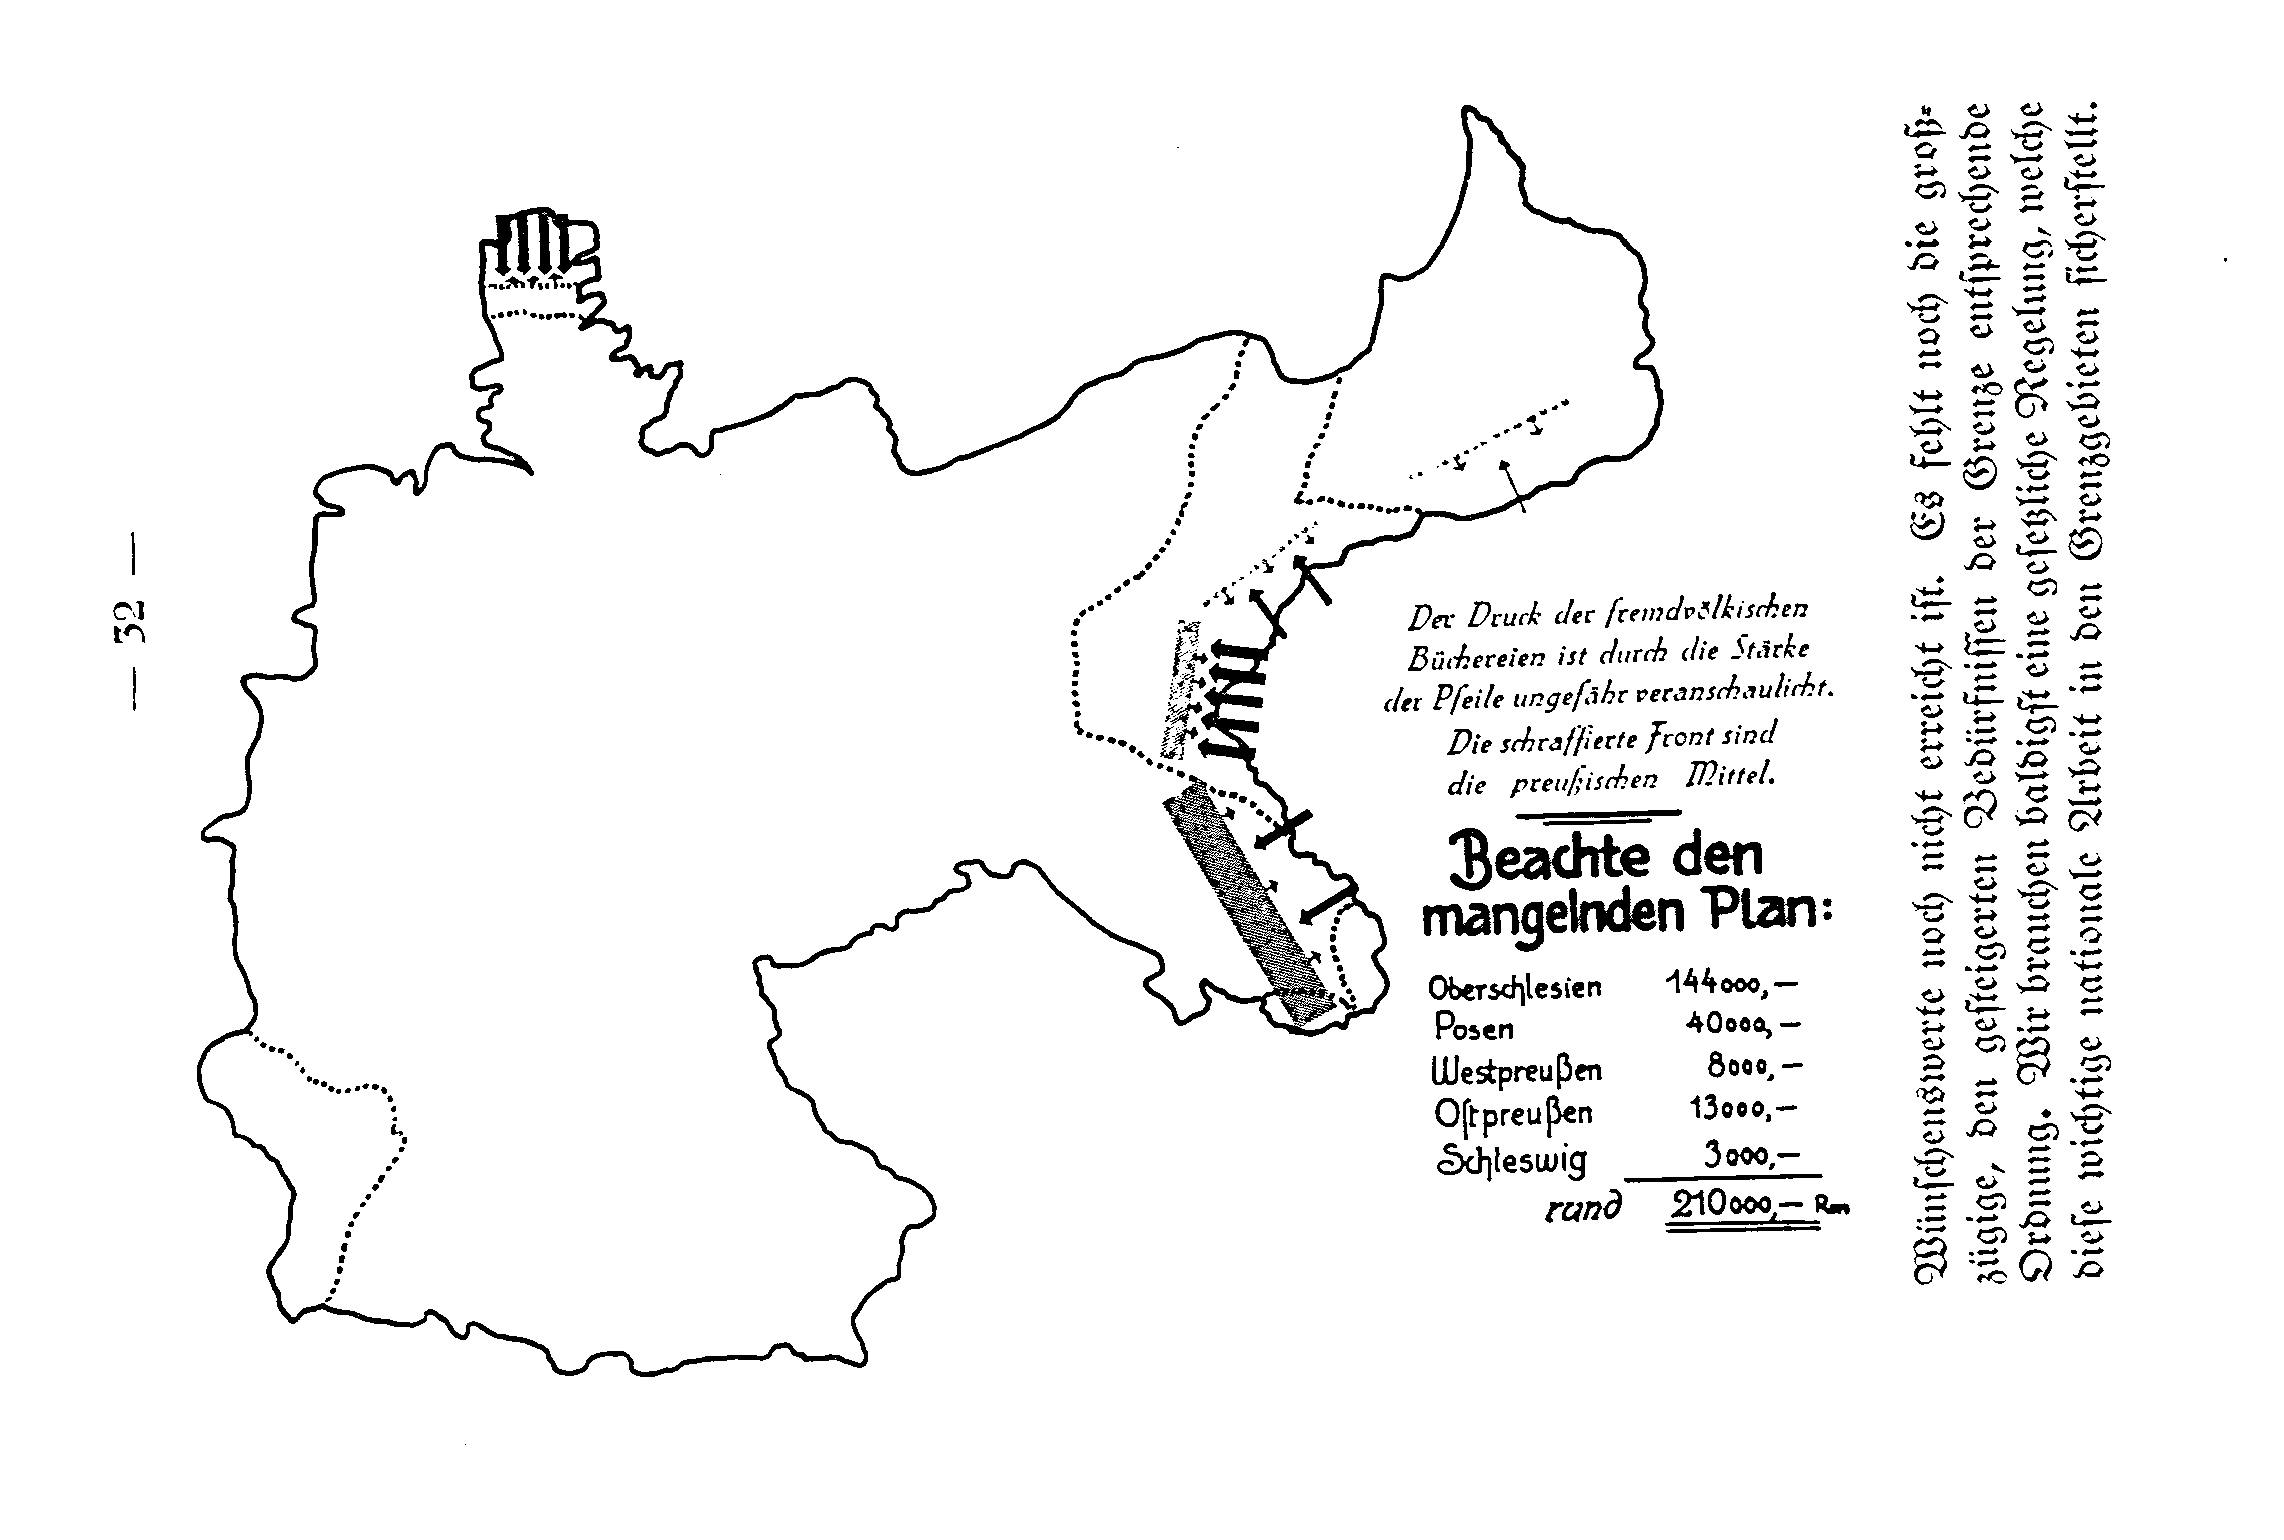
\includegraphics{img/karte_angriffe.jpg}
\caption{Karte aus Schriewer (1933b: 32). Die Karte zeigt das Deutsche
Reich nicht in den 1933 aktuellen Grenzen, sondern denen von 1914.
(Danzig, 1933 noch explizit «Freie Stadt» unter Völkerbundmandat, wenn
auch mit NSDAP-Regierung, ist gar nicht erst eingetragen.) In ihnen
abgetragen sind die angeblichen «Angriffe» dänischer und polnischer
Büchereiwesen und die -- angeblich -- zu geringen Verteidigungen von
deutscher Seite. Die Herkunft der Zahlen ist nicht klar (auch nicht,
warum angebliche «Angriffe» aus anderen Ländern nicht eingetragen sind),
aber es scheint, als würde einfach der Etat für die Förderung der
jeweiligen Büchereiwesen übersetzt in quasi militärische Aufgebote, die
sich in einer Schlachtordnung gegenüberstehen.}
\end{figure}

In den folgenden Jahren bis zum Beginn des Zweiten Weltkrieges
veränderte sich die konkrete Arbeit des Vereins nur leicht. Soweit
sichtbar, wurden weiterhin Bücher verschickt, Bücherlisten erstellt und
Büchereien beraten. Die Tagungen wurden, wie dargestellt, zu Fahrten
ausgebaut, bei denen «die Grenze» erfahrbar werden sollte. In den
\emph{Mitteilungen} wurden zudem «neue» Methoden der Büchereiarbeit
propagiert, beispielsweise der gezielte Einsatz von Lesungen.
Gleichzeitig scheint die Zusammenarbeit von Beratungsstellen und anderen
staatlichen Stellen noch enger geworden zu sein. Praktisch auf allen
Fahrten waren sie vertreten, gaben Arbeitsberichte und publizierten auch
in den \emph{Mitteilungen} selbst. Es scheint, als wäre der Verein
erfolgreich in das nationalsozialistische System integriert gewesen --
er hatte sich selbst gleichgeschaltet.

Ob dies für alle im Verein Aktiven galt, kann aufgrund der vorliegenden
Quellen nicht geklärt werden. Das könnte nur durch bibliographische
Studien geschehen. Es ist also denkbar, dass einzelne Personen einen
anderen Weg gingen oder aber ganz aus dem Büchereiwesen ausgeschlossen
wurden. Aber gesamthaft für den Verein gilt dies nicht.

\hypertarget{letzter-bruchpunkt-zweiter-weltkrieg}{%
\subsection{4.3 Letzter Bruchpunkt: Zweiter
Weltkrieg}\label{letzter-bruchpunkt-zweiter-weltkrieg}}

Der letzte Bruchpunkt der Vereinsgeschichte scheint der Beginn des
Zweiten Weltkrieges gewesen zu sein. Die letzte Publikation über die
konkrete Arbeit, zur Grenzbüchereifahrt nach Klagenfurt, also das dann
gerade angeschlossene Österreich, erschien 1939. (Scheffen-Döring 1939b,
Wille 1939) Danach taucht der Verein offenbar nur noch einmal mit einem
schon weiter oben genannten Beitrag von Wilhelm Schuster (Schuster 1940)
in den betreffenden Fachzeitschriften auf. Anschliessend scheint er
seine Aktivitäten eingestellt zu haben -- wohl mit der Vorstellung, sie
nach dem Ende des Krieges und einem Sieg des nationalsozialistischen
Deutschland wieder aufnehmen zu können. Aber der genaue Ablauf dieses
Endes lässt sich heute nicht mehr vollständig rekonstruieren. Ein
Nachlass des Vereins scheint nicht zu existieren. (Er wird zumindest in
den relevanten Archiven nicht nachgewiesen.) Was aber bekannt ist, ist,
dass eine ganze Anzahl von zuvor im «Grenzbüchereidienst» tätigen
Personen in die deutsche Wehrmacht eingezogen wurden. Hier ist wieder
Franz Schriewer als Beispiel zu nennen, der ab 1939 im Militär diente
(allerdings in Frankfurt/Oder selber) und für einige Jahre nicht mehr
gross als Autor in den relevanten Fachzeitschriften auftrat (Weimar
1976; gleichwohl aber mit eigenständigen Publikationen, vergleiche
Danker 2017).

Es scheint, als wäre die Arbeit des Vereins mit dem Beginn des Zweiten
Weltkrieges oder aber in dessen Verlauf eingestellt worden. Nach dem
Ende des Nationalsozialismus wurde er -- im Gegensatz zu vielen der
Staatlichen Fachstellen, mit denen er verbunden war -- nicht
weitergeführt oder wiedergegründet. Er scheint mit dem Regime
untergegangen zu sein. Dies gilt, wie auch schon thematisiert, nicht für
die Aktiven selbst. Diese fanden sich in vielen Fällen in den
Folgejahren vor allem im Büchereiwesen der westlichen Besatzungszonen
und dann der Bundesrepublik Deutschland wieder und besetzten dort
einflussreiche Positionen. Um dies nochmal an Franz Schriewer zu zeigen:
Er kehrte nach dem Zweiten Weltkrieg wieder nach Flensburg zurück und
wurde praktisch wieder in seine alte Position eingesetzt. In den
Folgejahren baute er das Büchereiwesen in Schleswig-Holstein neu auf,
schrieb jetzt aber zum Beispiel eher von der «Büchereilandschaft
Schleswig» (Schriewer 1958) und richtet sich auch nicht gegen die
dänische Kultur- und Büchereipolitik. Gleichwohl tat er dies zum Teil
weiter unter dem Schlagwort der «Grenzbüchereiarbeit». (Siehe den
Reihentitel der Schrift zur «Büchereilandschaft Schleswig» (Schriewer
1958): «Jahresbericht für das Grenzbüchereiwesen».) Danker (2017)
beschreibt diese Arbeit -- inklusive des damaligen Kontexts, unter
anderem der «Neudänischen Bewegung» -- biographisch als Fortsetzung der
bisherigen Arbeit Schriewers, bei gleichzeitiger Schuldabwehr; aber auch
als Versuch, sich in den neuen Verhältnissen zu orientieren. Wenn
Schriewer im vorliegenden Artikel als Beispiel für das deutsche
Volksbüchereiwesen gilt, dann auch damit.

\hypertarget{bewertung-und-fazit}{%
\section{5. Bewertung und Fazit}\label{bewertung-und-fazit}}

\hypertarget{politische-und-moralische-fragen}{%
\subsection{5.1 Politische und moralische
Fragen}\label{politische-und-moralische-fragen}}

Wie lässt sich die Geschichte des Vereins für Grenzbüchereidienst im
Rückblick bewerten? Zuerst ist selbstverständlich klar, dass diese
Arbeit grundsätzlich politisch falsch war: Die Vorstellungen von
Völkern, die gewissermassen als eigenständige Entitäten über den
Menschen und Staaten stehen und die sich gegenseitig bekämpfen, ist
nicht in der Realität gegründet. Was genau unter dem Begriff «Volk»
verstanden werden kann und wie sich kulturelle Identitäten innerhalb
eines Staates oder über verschiedene Staaten hinweg entwickeln, ist eine
bis heute offene Frage. Auch, was diese Kulturen, die im völkischen
Denken als eigenständige Entitäten «Volk» verstanden wurden,
«zusammenhält» oder gerade nicht zusammenhält, ist nicht eindeutig zu
klären. Ebenso ist nicht einfach zu klären, wann, wie und wieso Menschen
eine Kultur, die sie prägte, im Laufe der Zeit verändern, «verlassen»
oder eine neue Kultur annehmen. Klar ist aber, dass dies weder
ausschliessend passiert -- also dass Menschen sehr wohl Teil
verschiedener Kulturen sein können, als auch mehrere Kulturen innerhalb
eines Staates oder einer Region miteinander koexistieren können --, noch
dass sich diese Kulturen per se «bekämpfen».

Sicherlich gab und gibt es Fälle, in denen versucht wurde, Kulturen zu
vernichten -- aber nicht, weil dies in anderen Kulturen so angelegt ist,
sondern als Ergebnis staatlicher Interessen und Politik. Alleine in
Europa -- selbst, wenn man den von Europa ausgehenden Kolonialismus
ausblendet -- gibt es zahlreiche Beispiele dafür. Beispielsweise die
Politik der Assimilierung gegen die Kultur der Samen in Skandinavien
oder die bis heute anhaltenden Auseinandersetzung zwischen französischen
Staat und identitären Bewegungen in Korsika und dem Languedoc, die sich
zum Beispiel um Fragen von Kultur und Sprache, aber auch um ökonomische
Themen drehen. Historisch gab es zudem weit gewalttätigere
Auseinandersetzungen, die bis heute nicht vollständig beendet sind, wie
in Nordirland oder dem Baskenland. Aber auch die sorbische Kultur und
ihre Behandlung durch die jeweiligen deutschen Staaten kann hier als
Beispiel herangezogen werden. Doch die Vorstellung, dass dies immer so
sein muss und praktisch «in der Natur der Völker» angelegt wäre, ist
offensichtlich falsch.

Sowohl die sorbische Kultur als auch, um noch einmal auf dieses Beispiel
zurückzukommen, die dänische Kultur in Schleswig-Holstein heute, zeigen,
dass immer auch ein ganz anderes Denken über «Völker» möglich war und
ist. Auch ohne bis zu Ende zu klären, ob es überhaupt übergreifende
«Volkskulturen» gibt und wie Menschen auf diese bezogen werden sollten,
hat sich heute in Europa als Grundsatz etabliert, dass Minderheiten und
deren Kulturen geschützt werden müssen und dass ihnen Möglichkeiten
geboten werden müssen, sich zu entwickeln. Man hätte also in
Schleswig-Holstein immer auch ein Büchereiwesen aufbauen können, dass
sich gleichzeitig an Menschen richtet, welche sich zur deutschen, zur
dänischen, zu einer deutsch-dänischen, einer schleswigschen
Regionalkultur oder auch zu anderen Kulturen zugehörig fühlen. Die
Tschechoslowakei hatte dies nach 1918 mit ihrem Büchereigesetz versucht.
(Tschechoslowakei 1928) Aber dies wurde, wie gesagt, vom Verein als
Gefahr, nicht als mögliches Vorbild diskutiert. (Scheffen 1928a)

Schaut man mit diesem Wissen auf die Arbeit des «Grenzbüchereidienstes»
zurück, fällt aber auch eine Parallele auf: Kultur und Bücher wurden als
Werkzeug zur «Erhaltung» des Volkstums angesehen. Deutsche Bücher
sollten die deutsche Kultur und die deutsche Sprache erhalten. Ein
Ansatz heute, um Kulturen von Minderheiten zu fördern, ist weiterhin die
Förderung von Kultur und Literatur. Heute werden sowohl
sorbischsprachige als auch -- um ein weiteres Beispiel anzuführen --
rätoromanische Verlage und Publikationen finanziell unterstützt. Im
Gegensatz zum Grenzbüchereidienst aber ist diese Kulturförderung nicht
möglichst hegemonial gedacht, sondern als Ergänzung in einer
Kulturlandschaft, in welcher jeweils Publikationen verschiedener
Sprachen und Kulturen nebeneinander stehen.\footnote{Nicht explizit
  thematisiert wurde hier im Text, dass in der Grenzbüchereiarbeit auch
  explizit gegen «zu viele» Übersetzungen aus anderen Kulturen
  argumentiert wurde. (Vergleiche Schmitz 1928) In Besprechungen wurde
  aber zum Beispiel immer wieder auch abgewogen, ob bestimmte übersetzte
  Texte überhaupt in Büchereien «eingesetzt» werden sollten oder , ob
  sie vielleicht nur für Grossstadtbüchereien geeignet wären, nicht aber
  für völkisch homogener gedachte Dörfer.} Verbunden sind diese beiden
Ansätze aber darin, dass der Kultur und der Literatur eine starke Rolle
in Bezug auf Kultur zugeschrieben wird -- aber unter sehr anderen
Vorzeichen.

In diesem Text sollte es explizit nicht darum gehen, einzelne Aktive zu
bewerten. Und dennoch drängt sich die Frage auf, wie deren Arbeit
moralisch zu bewerten ist. War sie einfach zeitgenössisch, also «das,
was alle sagen» und deshalb von heute aus einfacher zu verurteilen, als
in der damaligen Zeit?

Dazu zwei kurze Anmerkungen: Erstens wurde weiter oben betont, dass das
völkische Denken und die nationalsozialistische Ideologie nicht per se
gleichgesetzt werden können. Man kann also nicht direkt aus der
Geschichte ab 1933 die Denkweisen und Handlungen völkischer Aktiver vor
1933 verurteilen. Aber, was auch sichtbar wurde, war, dass sich der
Verein 1933 sehr einfach und direkt in das nationalsozialistische System
integrieren lies. Offenbar gab es keinen Widerstand, sondern ein
Anpassen und Weitermachen. Das Denken der Aktiven war offenbar nur wenig
vom nationalsozialistischen entfernt -- die rassistische Vorstellung vom
Volk wurde schnell übernommen, Formen demokratischer oder offenerer
Mitbestimmung (also zum Beispiel der Vereine, welche die konkreten
Büchereien vor Ort führten) wurden schnell gegen eine zentralisierende,
autoritär organisierte Struktur («Führerprinzip») getauscht.

Zweitens gab es immer Alternativen, auch zeitgenössisch. Niemand war bis
1933 gezwungen, völkisch zu denken. Das völkische Denken wurde ja selber
als Alternative gegen internationalistische Denkweisen verstanden,
insbesondere in der organisierten Arbeiter*innenschaft und im
politischen Katholizismus. (Abgesehen davon, wie internationalistisch
diese beiden Milieus tatsächlich waren.) Das schon angeführte Beispiel
der Tschechoslowakei, die eine aktive Minderheitenpolitik betrieb, war
seit 1918 ebenso immer sichtbar. Aber auch in der deutschen Literatur
zum Volksbüchereiwesen selber finden sich Gegenbeispiele. In den
\emph{Mitteilungen} des Vereins findet sich ein Bericht über die Arbeit
der bayerischen Beratungsstelle (Fischer 1928), in dem die Probleme der
Büchereien im «Grenzgebiet» als die von Einrichtungen in -- wie man
heute sagen würde -- infrastrukturschwachen Regionen dargestellt werden.
Es geht darin um Infrastruktur, Personal, Etat und so weiter, aber nicht
um völkische Überlegungen. Das wäre also auch immer möglich gewesen.

Als Erwin Ackerknecht -- ein vielleicht noch produktiverer Autor als
Franz Schriewer -- 1930 in einem Artikel die mögliche Nutzung von
Schallplatten auf Bildungsveranstaltungen in Volksbüchereien besprach,
nutzte er dazu eine Sprache, die teilweise ähnlich der klingt, wie die,
welche in den \emph{Mitteilungen} des Verein genutzt wurde. Zudem nutzt
er Begrifflichkeiten, die heute als explizit rassistisch gelten:

\begin{quote}
«Eine außerordentliche Erweiterung ihres musikalischen und zugleich
völkerpsychologischen Horizontes wird vielen durch die fremdländische
Musik ermöglicht werden, die in Gestalt von Schallplatten zu haben ist.
Ich denke hier nicht so sehr an die Unmenge mehr oder weniger echter
Nigger-Songs, Tangos usw., obwohl selbstverständlich auch unter dieser
gelegentlich ein in seiner Art ‹ernst zu nehmendes› Stück ist. (So habe
ich für meine Person immer neuen Vergnügen an dem virtuos harmonisierten
Kater-Minnesang der beiden Negerquartette ‹Oh Lucindy› und ‹Ol` man
river› Electrola EB 916). Ich denke auch nicht in erster Linie an die
Kosakenchöre, von denen es eine ganze Reihe schöner Aufnahmen gibt.
Vielmehr liegt mir besonders daran, auf die hebräischen Gesänge
aufmerksam zu machen, die in der Wiedergabe durch den stimmgewaltigen
Kantor Rosenblatt selbst einem Antisemiten in vorgerücktem Stadium ans
Herz greifen müssten. {[}...{]}» (Ackerknecht 1930: 10)\footnote{Es
  folgen noch eine Reihe von anderen internationalen Aufnahmen,
  inklusive dem Wort «Zigeunerkapelle», bevor Ackerknecht dann zum
  eigentlichen Thema des Artikels übergeht.}
\end{quote}

Wie an diesem Zitat leicht nachzuvollziehen ist, steht diese Sprache bei
Ackerknecht im Dienst eines ganz anderen Denkens. Auch er geht wohl
davon aus, dass Völker irgendwie untereinander verschieden sind, aber
weder sieht er sie hier als miteinander kämpfende Entitäten, noch
scheint er «das eigene Volk» (das wäre bei Ackerknecht das deutsche)
bevorzugen zu wollen. Im Gegenteil, er plädiert für die Macht der Musik
als Mittel zur Verständigung zwischen den Menschen, die sogar «einem
Antisemiten in vorgerücktem Stadium» (Ackerknecht 1930: 10) ergreifen
müsste. Der Artikel von Ackerknecht ist in der gleichen Zeitschrift
\emph{Bücherei und Bildungspflege} erschienen, in der auch viele
Beiträge von Franz Schriewer publiziert wurden. Es war also auch nicht
die zeitgenössische Sprache alleine, die irgendwie das völkische Denken
erzwungen hätte. Es war immer auch möglich, mit dieser Sprache
inhaltlich gänzlich andere Ideen auszudrücken.

Ein weiteres Beispiel ist die Eröffnungsansprache, die Wilhelm Schuster
als Vorsitzender des \emph{Verbandes Deutscher Volksbibliothekare} (dem
dominierenden Verband der deutschen Volksbüchereiwesens) auf der
Jahrestagung von 1929 hielt -- also zu einer Zeit, in welcher der
\emph{Grenzbüchereidienst} selber sich eindeutig zu völkischen
Prinzipien bekannt hatte. In der Rede geht es um das Verhältnis von
Büchereien und weiterer Kulturarbeit. Für unseren Zusammenhang
interessant ist, dass Schuster dies mit einem eindeutigen positiven
Bezug «zur demokratischen sozialen Republik» (Schuster 1929a: 386), also
der Weimarer Republik, tat. Er bezeichnet sie, inklusive ihrer
politischen Strukturen zur Aushandlung von Differenzen, als
fortschrittlichste der existierenden Staatsformen. Ein solches
Bekenntnis, dass die Demokratie nicht einfach als Parteienstreit abtat,
über dem eine angebliche grössere «völkische» Idee stand, war damals im
Büchereiwesen auch von höchster Stelle aus möglich. (Obgleich es 1933
dann Schuster war, welcher das Büchereiwesen und den Verband relativ
reibungslos in den nationalsozialistischen Staat integrierte.)

Beachtet man dies, dann kann man die Denk- und Argumentationsweisen der
Aktiven in der Grenzbüchereiarbeit eben doch auch moralisch verurteilen:
Sie hatten offenbar immer Alternativen, aber sie wählten eine explizit
völkische Denkweise. Ob sie dieser auch nach 1945 verpflichtet waren
oder sich anderen, demokratischen Prinzipien zuwandten, ist eine andere
Frage. Schaut man sich aber die Entwicklung des schleswig-holsteinischen
Büchereiwesens, wieder unter Franz Schriewer, nach 1945 an, dann scheint
ein solcher Sinneswandel bei einigen wohl eingetreten zu sein.
(Schriewer 1958) Es stand dann beispielsweise nicht mehr kontinuierlich
unter dem Eindruck, einen «dänischen Einfluss» abwehren zu müssen.

Ein erstaunlicher Punkt ist, dass sich zumindest in den für diesen
Artikel hier gesichteten Schriften des Vereins -- im Gegensatz zu
sonstigen völkischen Publikationen -- kein konkreter Antisemitismus
findet. Sicherlich, implizit war er im völkischen Denken immer angelegt.
Eventuell wurde er nicht erwähnt, weil sich der Verein vor allem mit dem
ländlichen Raum befasste, der als einigermassen ausserhalb der
kapitalistischen Entwicklungen stehend gedacht wurde; während diese
Entwicklungen im Antisemitismus bekanntlich «den Juden» und «der
Grossstadt» zugeschrieben wurden. Aber vielleicht gehörten die im Verein
Aktiven tatsächlich zu dem kleinen Teil der Völkischen, die eine andere
Position zum Antisemitismus einnahmen. (Puschner, Schmitz \& Ulbricht
1996a) Letztlich hat dieses «Fehlen» die meisten Aktiven aber nicht
daran gehindert, sich später im explizit antisemitischen
nationalsozialistischen System zu engagieren.

\hypertarget{zum-erfolg-der-grenzbuxfcchereiarbeit}{%
\subsection{5.2 Zum Erfolg der
Grenzbüchereiarbeit}\label{zum-erfolg-der-grenzbuxfcchereiarbeit}}

Aber: War der \emph{Grenzbüchereidienst} erfolgreich? Hundertausende,
wohl eher Millionen von Büchern wurden im Laufe seines Bestehens
verschickt. Tausende, wenn nicht zehntausende, potentielle
Bibliothekar*innen wurden beraten, kontaktiert und mit Informationen
versorgt. Tagungen wurden durchgeführt, Grundbestandslisten für
Büchereien erstellt und verschickt (auch hier ist die konkrete Zahl
nicht mehr feststellbar, aber die Listen scheinen alle kostenlos
verschickt worden zu sein, insoweit ist von einem hohen Verbreitungsgrad
auszugehen). Publikationen wurden verbreitet. Grenzwissenschaftliche
Bibliotheken wurden aufgebaut und betrieben. Es wurden Kontakte zu den
entstehenden Beratungsstellen aufgebaut, sowie offenbar auch Kontakte zu
staatlichen Stellen und anderen potentiellen Geldgebern
aufrechterhalten.

Und trotzdem ist die Frage nicht zu klären, ob all diese Arbeit
tatsächlich Erfolg hatte. Wurden die verschickten Bücher überhaupt
aufgestellt? Wurden sie verliehen? Und wenn ja, hatten sie den
erwünschten «völkischen» Erfolg? Fühlten sich Menschen durch sie
«deutsch»? Ordneten sie sich den völkischen Gedanken unter und
entschieden sich zum Beispiel dafür, «im Dorf zu bleiben», um «deutschen
Boden» zu bewirtschaften? Oder wurden die Bücher vielleicht nur als
weiterer «Lesestoff» neben anderen Publikationen genutzt? Wurden die
Grundbestandslisten benutzt -- und wenn ja, von wem und wofür?
Entstanden, wie sich erhofft wurde, aus den Büchersendungen
eigenständige Büchereien, die dann vor Ort von lokalen Vereinen oder von
den Gemeinden getragen wurden? Hat der Verein durch seine Kontakte und
seine Beratungen vielleicht dafür gesorgt, dass moderne Büchereien
eingerichtet und professionell geführt wurden? Oder waren die vielen
Sendungen auch deshalb möglich, weil sich solche örtlichen Büchereien
nicht bildeten, also viele Gemeinden immer «Neuland» blieben und immer
neue Büchersendung «aufnehmen» konnten?

In den \emph{Mitteilungen} wurden Statistiken einzelner Büchereien
abgedruckt oder auch aus begeisterten Briefen an den Verein zitiert.
Aber ansonsten ging es in den Publikationen zur «Grenzbüchereiarbeit»
erstaunlich wenig um die konkrete Realität vor Ort. Letztlich wird es
wohl nur durch ganz konkrete Lokalstudien möglich sein, wenn überhaupt,
zu klären, welchen Einfluss die Arbeit des Vereins in den einzelnen
Gemeinden und bei den Menschen vor Ort tatsächlich hatte.

Fest steht, dass die staatlichen Beratungsstellen für Büchereien, mit
denen der Verein zusammenarbeitete, in vielen Fällen bis heute weiter
existieren, zumindest dort, wo sie heute nicht auf dem Gebiet anderer
Staaten liegen.\footnote{Es wäre eine interessante Fragestellung, ob
  sich zum Beispiel im polnischen Öffentlichen Bibliothekswesen heute
  noch Strukturen finden, die damals aufgebaut wurden. Aber das ist
  nicht im Fokus dieses Artikels.} Grundsätzlich existieren solche heute
in allen Bundesländern Deutschlands und Österreichs. Aber: Ist das ein
Ergebnis der Arbeit des Vereins? Oder hat der Verein hier nicht auf eine
Entwicklung zur «Erhöhung der Staatsquote» im Volksbüchereiwesen
reagiert, die auch ohne ihn eingetreten worden wäre? Hat das völkische
Denken die Struktur der Beratungsstellen und ihrer Arbeit geprägt -- und
wenn ja, wirkt das heute noch nach? Auch dies ist ohne konkrete
Lokalstudien schwer zu bestimmen und wird auch dann nur schwierig zu
beantworten sein, da -- wie erwähnt -- oft die Leiter der
Beratungsstellen gleichzeitig im Verein aktiv waren. Wer hat in solchen
Fällen dann wen beeinflusst? Zu vermuten ist aber, dass dieser Einfluss
in der Realität recht klein war. Dabei, das sollte noch festgehalten
werden, war die Situation in Deutschland in den 1920er und 1930er Jahren
an sich davon gekennzeichnet, dass das Verhältnis von Vereinen, privaten
Initiativen, Gesellschaft, Wirtschaft und Staat grundsätzlich neu
ausgehandelt wurde, nicht nur im Volksbüchereiwesen. Die Gründung der
Republiken, die entstehenden politischen Bewegungen, kurz: die
gesellschaftliche Modernisierung machten dies notwendig. Das es am
Anfang der 1920er Jahre sinnvoll erschien, dass Vereine die Hauptarbeit
im Büchereiwesen trugen und dass gleichzeitig noch nach stabilen Formen
für eine langfristige Struktur zur Unterstützung dieser Büchereien
gesucht wurde, während im Laufe der 1920er Jahre der Staat mehr
Verantwortung übernahm, war zeitgenössisch. Dies passierte auch in
anderen Bereichen. (Vergleiche Pöggler (1974) für die
Erwachsenenbildung, insbesondere die Volkshochschulen, und Feldmann
(1975) für den relativ bald gescheiterten Versuch, in den frühen 1920er
Jahren eine Arbeitsgemeinschaft von Industrieverband und Gewerkschaften
zu etablieren.) Eventuell wäre der Verein ohne den Nationalsozialismus
also irgendwann vollständig eine staatliche Struktur geworden und hätte
seinen völkischen Fokus verloren. Unter Umständen wäre die
Grenzbüchereiarbeit irgendwann zu einer Büchereiförderung in
strukturschwachen Gebieten geworden. Dann wäre sein Vermächtnis unter
Umständen positiver zu bewerten.

Insoweit muss man am Ende aber feststellen, dass der Verein über lange
Zeit ernstgemeinte und auch an den Entwicklungen des damaligen
Volksbüchereiwesens orientierte Arbeit geleistet hat sowie dafür eine
grosse Masse an Ressourcen mobilisieren konnte, aber das die konkrete
Wirkung dieser Arbeit nicht mehr nachzuweisen ist.\footnote{Eine weitere
  offene Frage ist, ob und wie dies in den anderen Ländern passierte.
  Vom Verein und anderen Aktiven im deutschen Volksbüchereiwesen wurde
  kontinuierlich unterstellt, dass die anderen Staaten ihr Büchereiwesen
  mit den gleichen Zielen einsetzen würden, wie dies vom Verein
  angedacht wurde. Interessant wäre zu untersuchen, ob dies stimmt oder
  ob in anderen Ländern andere Ziele vorherrschten.}

\hypertarget{abschliessende-bewertung}{%
\subsection{5.3 Abschliessende
Bewertung}\label{abschliessende-bewertung}}

Geschichte hat keine Moral per se, aber es lässt sich dennoch aus ihr
lernen. Was die Geschichte der Grenzbüchereiarbeit für das heutige
Bibliothekswesen zeigt, ist, dass Öffentliche Bibliotheken nicht von
sich aus für eine politische Richtung oder Denkweise stehen. Der Verein
konnte die ganze Zeit seines Bestehens über davon ausgehen, dass seine
Arbeit (die Grundlisten, die verschickten Bücher, die Beratung zum
Aufbau moderner Büchereien) mit seinen politischen Grundüberzeugungen
übereinstimmte. Er wollte ein völkisches Büchereiwesen aufbauen und
später dann den Aufbau eines nationalsozialistischen Büchereiwesens
unterstützen. Dabei stand er, was den bibliothekarischen Diskurs und die
verwendeten Techniken betrifft, vollkommen im Mainstream des damaligen
deutschen Büchereiwesens. Einige der Personen -- um noch einmal auf
Franz Schriewer zu verweisen -- waren sogar das, was man heute
Innovator*innen nennen würde, welche diese Techniken (vergleiche
Schriewer (1924) zu den Büchereilehrgängen, die er organisierte sowie
Schriewer (1925) zur Unterbringung kleiner Sammlungen in speziellen
Bücherschränken) und die Reflexion über die Arbeit in Büchereien (siehe
Schriewer (1926) zur Kritik an zu geringer Beachtung lokaler
Gegebenheiten bei der Planung und Anleitung von Bibliotheken)
vorantrieben. Einerseits lässt sich dies auf das völkische
Selbstverständnis, Teil der modernen Gesellschaft zu sein und diese
verändern zu wollen, zurückführen. Andererseits zeigt dies auch, dass
inhaltlich falsche Ideen über die Gesellschaft nicht davon abhalten,
Büchereien weiterzuentwickeln. Es gibt keine direkte Verbindung von
«richtigen Ideen» über die Gesellschaft und der jeweiligen
Bibliotheksarbeit -- vielmehr sind Volksbüchereien, oder heute
Öffentliche Bibliotheken, Einrichtungen, die von verschiedenen
politischen Richtungen betrieben und weiterentwickelt werden können.

Zwei Dinge fallen zudem auf. Erstens war es im völkischen Büchereiwesen
während der Weimarer Republik normal, zu behaupten, eine gewisse
neutrale Position «über den Parteien» einzunehmen. Wie auch in anderen
völkischen Gruppierungen legte man Wert darauf, alle Teile «des Volkes»
ansprechen zu wollen und angeblich auch repräsentieren zu können.
Unterschiede, ob politische oder soziale, wurden als nebensächlich
bezeichnet, welche die «überzeitliche Wahrheit» des Volkes nicht
tangieren würden. Gleich mit Beginn des nationalsozialistischen Regimes
wurde, wie gezeigt, eine neue Argumentation formuliert, nämlich dass
dies immer eine Schutzbehauptung gewesen wäre, um auch in der Demokratie
völkische Politik betreiben zu können. Aber es ist davon auszugehen,
dass zumindest für einen Teil der Aktiven für eine lange Zeit während
der Weimarer Republik diese Vorstellung, einigermassen neutral zu sein,
prägend war. Nicht alle werden das nur «vorgeschoben» haben. Das führt
zu der Frage, wie spätere, auch heute noch verbreitete, Vorstellungen
von einer «Neutralität» der Öffentlichen Bibliotheken zu bewerten sind.
Sind das auch Vorstellungen, die zwar von vielen geteilt werden, die
aber von einer bestimmten gesellschaftlichen Vorstellung geprägt sind?
Sind heutige Vorstellungen von Neutralität im Bibliotheksbereich nicht
eventuell auch davon geprägt, einen gemeinsamen (selbstverständlich
nicht völkischen) Zusammenhang innerhalb der Gesellschaft zu sehen, der
über den politischen Auseinandersetzungen und sozialen Differenzen
besteht? Der Neutralitätsgedanke im Bibliothekswesen ist in den letzten
Jahren mehrfach kritisiert worden, zum Beispiel aus antirassistischen
und antikolonialen, aber auch aus feministischen und anderen
Perspektiven. (Lewis 2008, Leyrer 2019, Wagner \& Crowley 2020, Hennicke
2021, Scott \& Saunders 2021) Die in diesem Artikel geschilderte
Geschichte ergänzt diese Kritik in gewisser Weise.

Und zweitens ist festzustellen, dass diese ganze Arbeit, welche der
Verein unternahm, inklusive der ganzen Ressourcen, die dafür mobilisiert
wurden, auf bestimmten Überzeugungen von der Wirksamkeit von Büchern und
Büchereien aufbaute. Obgleich es schwer zu klären ist, welche
tatsächliche Wirkung diese Arbeit hatte, gab es bei den Aktiven doch die
feste Überzeugung, dass durch sie «das Volkstum» gestärkt wurde oder das
«andere Völker» ihre jeweiligen Büchereien einsetzen würden, um ihr
«Volkstum» zu stärken. Mit Abstand von heute betrachtet erscheint das
eine nicht nachvollziehbare Vorstellungswelt, die sich vielleicht auch
dadurch erhalten konnte, dass ihre Realität empirisch kaum untersucht
wurde. In keinem einzigen Artikel in den \emph{Mitteilungen} wurde
jemals versucht, in den betreffenden Regionen beispielsweise mit
Umfragen, Beobachtungen oder -- was zeittypisch als sinnvoll gegolten
hätte -- Bevölkerungsstatistiken zu überprüfen, ob sich durch die
Büchereien das «völkische Bewusstsein» verändert hätte. Es wurde nur
immer und immer wieder behauptet.

Doch auch das wirft die Frage auf, wie es heute ist. Werden Öffentliche
Bibliotheken vielleicht auch heute betrieben auf der Basis bestimmter
Überzeugungen, die zwar wirkmächtig sind, aber kaum überprüft werden?
Wird zum Beispiel jemals gezeigt, dass die weit verbreitete
«Leseförderung» tatsächlich dazu führt, dass mehr, besser oder zumindest
gerne gelesen wird? Oder -- das würde dann heissen, dass Ideen eine
wichtige Rolle in der Bibliotheksarbeit spielen -- reicht die
Vorstellung aus, dass sie eine Wirkung haben? Auffällig ist, dass es
tatsächlich kaum Untersuchungen zu diesem Fragekomplex gibt. Sicherlich:
Leseförderung ist etwas anderes, als es die völkische
Grenzbüchereiarbeit war; sie ist etwas, das auch zu begrüssen wäre, wenn
es gar keine nachweisbare Wirkung hat. Aber in gewisser Weise scheint
hier auch eine Parallele zu bestehen. Die Vorstellung alleine, dass
Volksbüchereien beziehungsweise Öffentliche Bibliotheken eine bestimmte
Wirkung haben, führt dazu, dass (erstaunlich viele) Ressourcen für die
bibliothekarische Arbeit mobilisiert werden können.

\hypertarget{literatur}{%
\section{6. Literatur}\label{literatur}}

Ackerknecht, Erwin. 1918. \emph{Das Lichtspiel im Dienste der
Bildungspflege: Handbuch für Lichtspielreformer}. Berlin: Weidmann.

---------. 1922. «Wanderbücherei». \emph{Bücherei und Bildungspflege:
Zeitschrift für die gesamten außerschulischen Bildungsmittel} 2 (9):
185--96.

---------. 1926. \emph{Büchereifragen: Aufsätze zur Bildungsaufgabe und
Organisation der modernen Bücherei}. 2., Vermehrte Auflage. Berlin:
Weidmann.

---------. 1930. «Bildungspflege und Schallplatte». \emph{Bücherei und
Bildungspflege: Zeitschrift für die gesamten außerschulischen
Bildungsmittel} 10 (1): 7--15.

---------. 1933. «Büchereigesetzgebung». \emph{Bücherei und
Bildungspflege: Zeitschrift für die gesamten außerschulischen
Bildungsmittel} 13 (3): 171--85.

Albrecht, Dietmar. 2020. «Schriewer, Franz Wilhelm Friedrich». In
\emph{BioLex Digital: Biographisches Lexikon für Schleswig-Holstein und
Lübeck}, herausgegeben von Schleswig-Holsteinische Landesbibliothek,
2441--43. Kiel; Hamburg: Wachholtz Verlag.

Amm, Bettina. 2012. «Die Ludendorff-Bewegung im Nationalsozialismus -
Annäherung und Abgrenzungsversuche». In \emph{Die völkisch-religiöse
Bewegung im Nationalsozialismus: eine Beziehungs- und
Konfliktgeschichte}, herausgegeben von Clemens Vollnhals und Uwe
Puschner, 127--47. Schriften des Hannah-Arendt-Instituts für
Totalitarismusforschung 47. Göttingen: Vandenhoeck \& Ruprecht.

Andrae, Friedrich, Hrsg. 1970. \emph{Volksbücherei und
Nationalsozialismus: Materialien zur Theorie und Politik des
öffentlichen Büchereiwesens in Deutschland 1933-1945}. Beiträge zum
Büchereiwesen. Reihe B: Quellen und Texte 3. Wiesbaden: O. Harrassowitz.

Anonym. 1922. «Entwicklung und gegenwärtige Arbeit des Vereins zur
Verbreitung guter volkstümlicher Schriften E.V.» \emph{Mitteilungen des
Vereins zur Verbreitung guter volkstümlicher Schriften}, Nr. 5: 1--11.

---------. 1928. «Tagungen des ‹Grenzbüchereidienst und Bildungspflege
E.V.›: Zweite Grenzbüchereitagung in Chorinchen (Mark) vom 13.-15..
Oktober 1927 , Büchereilehrgang für evangelische Arbeitersekretäre in
Düsseldorf vom 12.-15. April 1928». \emph{Grenzbüchereidienst und
Bildungspflege}, Nr. 8: 80--87.

---------. 1936. «Volksbücherei-Kundgebung in Bayreuth».
\emph{Grenzbüchereidienst e.V. Mitteilungen}, Nr. 14: 11--28.

Barbian, Jan-Pieter. 2010. \emph{Literaturpolitik im NS-Staat: von der
Gleichschaltung bis zum Ruin}. Fischer Taschenbuch 16306. Frankfurt am
Main: Fischer Taschenbuch Verlag.

Boese, Engelbrecht. 1987. \emph{Das öffentliche Bibliothekswesen im
Dritten Reich}. Bibliothek und Gesellschaft. Bad Honnef: Bock und
Herchen.

Brajer, Sven. 2022. \emph{Am Rande Dresdens?: Das völkisch-national
Spektrum einer «konservativen Kulturstadt» 1879-1933}. Dresden; München:
Thelem Universitätsverlag.

Breuer, Stefan. 2010. \emph{Die Völkischen in Deutschland Kaiserreich
Und Weimarer Republik}. 2., Unveränderte Auflage. Darmstadt: WBG
Wissenschaftliche Buchgesellschaft.

Danker, Uwe. 2017. «Franz Schriewer: Volksbibliothekar, Referatsleiter
der Reichsstelle, Grenzkämpfer. Biographische Erkundungen 1921-1959». In
\emph{Volksbibliothekare im Nationalsozialismus: Handlungsspielräume,
Kontinuitäten, Deutungsmuster}, herausgegeben von Sven Kuttner und Peter
Vodosek, 67--118. Wolfenbütteler Schriften zur Geschichte des Buchwesens
50. Wiesbaden: Harrassowitz Verlag.

Engelhardt, Isabelle. 2015. «Der Kampf gegen die moralische Vergiftung:
Die Diskussionen um ‹Schund und Schmutz› in Film und Literatur». In
\emph{Diskursgeschichte der Weimarer Republik}, herausgegeben von
Thorsten Eitz und Isabelle Engelhardt, Band 2:261--312. Hildesheim;
Zürich; New York: Georg Olms Verlag.

Escher, Hermann. 1922. «Die schweizerische Volksbibliothek».
\emph{Wissen und Leben} 25: 227--35.
\url{https://doi.org/10.5169/seals-749915}.

Fahlbusch, Michael und Ingo Haar. 2020. «Einleitung: Das Völkische als
genuin deutschnationales Ideologem». In \emph{Völkische Wissenschaften:
Ursprünge, Ideologien und Nachwirkungen}, herausgegeben von Michael
Fahlbusch, Ingo Haar, Anja Lobenstein-Reichmann, und Julien
Reitzenstein, 1--13. Berlin; Boston: De Gruyter Oldenbourg.
\url{https://doi.org/10.1515/9783110654592}.

Fahlbusch, Michael, Ingo Haar, Anja Lobenstein-Reichmann, und Julien
Reitzenstein, Hrsg. 2020. \emph{Völkische Wissenschaften: Ursprünge,
Ideologien und Nachwirkungen}. Berlin; Boston: De Gruyter Oldenbourg.
\url{https://doi.org/10.1515/9783110654592}.

Feldhausen, Gg. 1910. «Die Kinder-Lesehalle in Wiesbaden». \emph{Blätter
für Volksbibliotheken und Lesehallen} 11 (5--6): 69--71.

Feldman, Gerald Donald. 1985. \emph{Industrie und Gewerkschaften
1918-1924: die überforderte Zentralarbeitsgemeinschaft}. Schriftenreihe
der Vierteljahrshefte für Zeitgeschichte 50. Stuttgart: Deutsche
Verlags-Anstalt.

Fischer, Anton. 1928. «Tätigkeitsbericht über die Grenzbüchereiarbeit
der bayerischen staatlichen Beratungsstelle für Volksbüchereien an der
Staatsbibliothek München». \emph{Grenzbüchereidienst und
Bildungspflege}, Nr. 8: 69--72.

Flachowsky, Sören. 2018. \emph{«Zeughaus für die Schwerter des Geistes»:
die Deutsche Bücherei in Leipzig, 1912-1945}. Göttingen: Wallstein
Verlag.

Fritz, Gottlieb, Erwin Ackerknecht und Wilhelm Schuster. 1933. «Zum
Abschied». \emph{Bücherei und Bildungspflege: Zeitschrift für die
gesamten außerschulischen Bildungsmittel} 13 (5): 329--30.

Hansen, Julie. 1914. «Ein Streifzug durch Londoner Volksbibliotheken.
Ostern 1914». \emph{Blätter für Volksbibliotheken und Lesehallen} 15
(9--10): 145--51.

Hartung, Günter. 1996. «Völkische Ideologie». In \emph{Handbuch zur
«Völkischen Bewegung» 1871-1918}, herausgegeben von Uwe Puschner, Walter
Schmitz, und Justus H. Ulbricht, 22--41. München; New Providence;
London; Paris: K.G. Saur.

Heiligenstaedt, Fritz. 1939. «Das Volksbüchereiwesen im nordöstlichen
Grenzraum». \emph{Grenzbüchereidienst e.V. Mitteilungen}, Nr. 16:
37--44.

Hennicke, Steffen. 2021. \emph{Neutralität in Bibliotheken}. Berliner
Handreichungen zur Bibliotheks- und Informationswissenschaft 479.
Berlin: Humboldt Universität zu Berlin, Institut für Bibliotheks- und
Informationswissenschaft.

Hesse, Charlotte von. 1928. «Bücherlisten des ‹Grenzbüchereidienst und
Bildungspflege E.V.›» \emph{Grenzbüchereidienst und Bildungspflege}, Nr.
8: 64--68.

---------. 1931. «Wie tun wir Grenzbüchereidienst?»
\emph{Grenzbüchereidienst und Bildungspflege}, Nr. 10: 55--72.

---------. 1937. «Werbeveranstaltung des Grenzbüchereidienstes E.V.
Berlin». \emph{Die Bücherei: Zeitschrift für Schriftumspflege} 4 (4--5):
230--33.

Hoffmann, Heike. 1996. «Völkische Kapitalismus-Kritik: Das Beispiel
Warenhaus». In \emph{Handbuch zur «Völkischen Bewegung» 1871-1918},
herausgegeben von Uwe Puschner, Walter Schmitz, und Justus H. Ulbricht,
558--71. München; New Providence; London; Paris: K.G. Saur.

Honigheim, Paul. 1923. «Der volkswirtschaftliche Lehrfilm».
\emph{Bücherei und Bildungspflege: Zeitschrift für die gesamten
außerschulischen Bildungsmittel} 3 (1): 20--26.

Kaisig, Karl. 1912. «Der Verband oberschlesischer Volksbüchereien».
\emph{Blätter für Volksbibliotheken und Lesehallen} 13 (5 / 6): 73--81.

Kander, Viktor. 1928. «Das deutsche Büchereiwesen in
Polnisch-Oberschlesien, Ostschlesien und Galizien». \emph{Bücherei und
Bildungspflege: Zeitschrift für die gesamten außerschulischen
Bildungsmittel} 8 (3): 169--72.

Kettel, Andreas. 1981. \emph{Volksbibliothekare und Nationalsozialismus:
zum Verhalten führender Berufsvertreter während der
nationalsozialistischen Machtübernahme}. Pahl-Rugenstein
Hochschulschriften. Gesellschafts- und Naturwissenschaften 72. Serie
Faschismusstudien. Köln: Pahl-Rugenstein.

Kock, Richard. 1934. «Die Neuordnung der Beratungsstellen». \emph{Die
Bücherei: Zeitschrift für Schriftumspflege} 1 (1): 18--29.

König, Fr.~1929. «Die Bedeutung der Außen- und Grenzdeutschen für die
deutsche Gesamtkultur». \emph{Grenzbüchereidienst und Bildungspflege},
Nr. 9: 26--49.

Kuttner, Sven, und Peter Vodosek, Hrsg. 2017. \emph{Volksbibliothekare
im Nationalsozialismus: Handlungsspielräume, Kontinuitäten,
Deutungsmuster}. Wolfenbütteler Schriften zur Geschichte des Buchwesens
50. Wiesbaden: Harrassowitz Verlag.

Langfeldt, Johannes. 1924. «Die Entwicklung der Volksbüchereien in
Dänemark». \emph{Bücherei und Bildungspflege: Zeitschrift für die
gesamten außerschulischen Bildungsmittel} 4 (2): 87--91.

---------. 1931. «Das neue dänische Büchereigesetz». \emph{Bücherei und
Bildungspflege: Zeitschrift für die gesamten außerschulischen
Bildungsmittel} 11 (4): 232--42.

---------. 1933. «Zentralisierende und dezentralisierende Auswirkungen
des dänischen Büchereigesetzes». \emph{Bücherei und Bildungspflege:
Zeitschrift für die gesamten außerschulischen Bildungsmittel} 13 (3):
188--94.

Lewis, Alison M. 2008. \emph{Questioning Library Neutrality: Essays from
Progressive Librarian}. Duluth, Minn: Library Juice Press.

Leyrer, Katharina. 2019. «Zur Unmöglichkeit eines neutralen
Bibliotheksangebots». \emph{LIBREAS. Library Ideas}, Nr. 35.
\url{https://libreas.eu/ausgabe35/leyrer/}.

Lindmaier, Irene. 1917. «Aus der Kriegsbücherei unseres Vereins».
\emph{Mitteilungen des Vereins zur Verbreitung guter volkstümlicher
Schriften}, Nr. 1: 10--14.

Linse, Ulrich. 1996. «Völkisch-rassische Siedlungen der Lebensreform».
In \emph{Handbuch zur «Völkischen Bewegung» 1871-1918}, herausgegeben
von Uwe Puschner, Walter Schmitz, und Justus H. Ulbricht, 397--410.
München; New Providence; London; Paris: K.G. Saur.

Maiwald, Georg. 1931. «Zur Frage der privaten Leihbibliotheken».
\emph{Bücherei und Bildungspflege: Zeitschrift für die gesamten
außerschulischen Bildungsmittel} 12 (2): 104--8.

Moucha, Anton. 1929. «Zehn Jahre tschechoslowakisches Büchereigesetz».
\emph{Bücherei und Bildungspflege: Zeitschrift für die gesamten
außerschulischen Bildungsmittel} 9 (5): 321--41.

Nachtigall, Herta. 1929. «Dritte Grenzbüchereitagung».
\emph{Grenzbüchereidienst und Bildungspflege}, Nr. 9: 80--87.

Pöggeler, Franz, Hrsg. 1974. \emph{Geschichte der Erwachsenenbildung}.
Handbuch der Erwachsenenbildung 4. Stuttgart: Kohlhammer.

Puschner, Uwe, Walter Schmitz, und Justus H. Ulbricht, Hrsg. 1996a.
\emph{Handbuch zur «Völkischen Bewegung» 1871-1918}. München; New
Providence; London; Paris: K.G. Saur.

---------. 1996b. «Vorwort». In \emph{Handbuch zur «Völkischen Bewegung»
1871-1918}, herausgegeben von Uwe Puschner, Walter Schmitz, und Justus
H. Ulbricht, IX--XXIII. München; New Providence; London; Paris: K.G.
Saur.

Rau, Christian. 2018. \emph{«Nationalbibliothek» im geteilten Land: die
Deutsche Bücherei, 1945-1990}. Göttingen: Wallstein Verlag.

Reinhold. 1921. «Gute volkstümliche Schriften aus den letzten Jahren».
\emph{Mitteilungen des Vereins zur Verbreitung guter volkstümlicher
Schriften}, Nr. 4: 37--43.

Retterath, Jörn. 2016. \emph{«Was ist das Volk?»: Volks- und
Gemeinschaftskonzepte der politischen Mitte in Deutschland 1917-1924}.
Quellen und Darstellungen zur Zeitgeschichte 110. Berlin; Boston: Walter
de Gruyter.

---------. 2020. «‹Volk ist etwas ganz anderes, als was bisher als
solches auftrat›: Volkskonzepte in der Völkischen Bewegung zu Beginn der
Weimarer Republik». In \emph{Völkische Wissenschaften: Ursprünge,
Ideologien und Nachwirkungen}, herausgegeben von Michael Fahlbusch, Ingo
Haar, Anja Lobenstein-Reichmann, und Julien Reitzenstein, 102--17.
Berlin; Boston: De Gruyter Oldenbourg.
\url{https://doi.org/10.1515/9783110654592}.

Roscher, Heinz. 1934. «Deutsches Büchereiwesen jenseits der
Reichsgrenze». \emph{Die Bücherei: Zeitschrift für Schriftumspflege} 1
(12): 537--42.

Rosenberger, Sebastian. 2020. «Oswald Spenglers ‹Der Untergang des
Abendlandes›. Eine völkische Geschichtsphilosophie?» In \emph{Völkische
Wissenschaften: Ursprünge, Ideologien und Nachwirkungen}, herausgegeben
von Michael Fahlbusch, Ingo Haar, Anja Lobenstein-Reichmann, und Julien
Reitzenstein, 118--39. Berlin; Boston: De Gruyter Oldenbourg.
\url{https://doi.org/10.1515/9783110654592}.

Ruppe, Hans. 1939. «Die neue Volksbücherei in der Ostmark». \emph{Die
Ostmarkbücherei: Mitteilungen der Staatlichen Volksbüchereistelle Wien}
1 (1--2): 4--8.

Scheffen, Wilhelm. 1920. «Grenzmarkbüchereien». \emph{Mitteilungen des
Vereins zur Verbreitung guter volkstümlicher Schriften}, Nr. 3: 1--8.

---------. 1921. «Buch und Kulturarbeit für das ringende Deutschtum».
\emph{Mitteilungen des Vereins zur Verbreitung guter volkstümlicher
Schriften}, Nr. 4: 1--16.

---------. 1928a. «Grenzbüchereiarbeit, Tatsachen und Ziele».
\emph{Grenzbüchereidienst und Bildungspflege}, Nr. 8: 5--20.

---------. 1928b. «Vorwort». \emph{Grenzbüchereidienst und
Bildungspflege}, Nr. 8: 3--4.

---------. 1933. «Grenzbüchereidienst in der Zeitenwende».
\emph{Grenzbüchereidienst e.V. Mitteilungen}, Nr. 12: 3--7.

---------. 1934. «Grenzbüchereiarbeit im preussischen Osten». \emph{Die
Bücherei: Zeitschrift für Schriftumspflege} 1 (7--8): 313--25.

Scheffen-Döring, Luise. 1935. «Reisebericht». \emph{Grenzbüchereidienst
e.V. Mitteilungen}, Nr. 13: 14--44.

---------. 1936. «Reisebericht». \emph{Grenzbüchereidienst e.V.
Mitteilungen}, Nr. 14: 29--60.

---------. 1938. «Tagungsbericht». \emph{Grenzbüchereidienst e.V.
Mitteilungen}, Nr. 15: 15--37.

---------. 1939a. «Tagungsbericht». \emph{Grenzbüchereidienst e.V.
Mitteilungen}, Nr. 17: 21--43.

---------. 1939b. «Tagungsbericht». \emph{Grenzbüchereidienst e.V.
Mitteilungen}, Nr. 16: 9--36.

Scherzberg, Lucia. 2012. «Katholizismus und völkische Religion
1933-1945». In \emph{Die völkisch-reli\-giöse Bewegung im
Nationalsozialismus: eine Beziehungs- und Konfliktgeschichte},
herausgegeben von Clemens Vollnhals und Uwe Puschner, 299--334.
Schriften des Hannah-Arendt-Instituts für Totalitarismusforschung 47.
Göttingen: Vandenhoeck \& Ruprecht.

Schmitz, D.A. 1928. «Zur Überfremdung des deutschen Buchmarktes».
\emph{Bücherei und Bildungspflege: Zeitschrift für die gesamten
außerschulischen Bildungsmittel} 8 (4): 236--38.

Schmitz, Wolfgang, und Michael Knoche, Hrsg. 2011.
\emph{Wissenschaftliche Bibliothekare im Nationalsozialismus:
Handlungsspielräume, Kontinuitäten, Deutungsmuster}. Wolfenbütteler
Schriften zur Geschichte des Buchwesens 46. Wiesbaden: Harrassowitz
Verlag.

Schriewer, Franz. 1923. «Büchereiwesen im deutschen und dänischen
Grenzgebiet». \emph{Bücherei und Bildungspflege: Zeitschrift für die
gesamten außerschulischen Bildungsmittel} 3 (4): 220--23.

---------. 1924a. «Büchereilehrgänge der Zentrale für
Nordmarkbüchereien». \emph{Bücherei und Bildungspflege: Zeitschrift für
die gesamten außerschulischen Bildungsmittel} 4 (2): 82--87.

---------. 1924b. «Der Schrank der Dorfbücherei». \emph{Bücherei und
Bildungspflege: Zeitschrift für die gesamten außerschulischen
Bildungsmittel} 4 (4): 188--93.

---------. 1924c. «Dorfbücherei und Bauernhochschule». \emph{Bücherei
und Bildungspflege: Zeitschrift für die gesamten außerschulischen
Bildungsmittel} 4 (1): 8--19.

---------. 1925a. «Eine Statistik ländlicher Büchereiarbeit».
\emph{Bücherei und Bildungspflege: Zeitschrift für die gesamten
außerschulischen Bildungsmittel} 5 (1): 1--11.

---------. 1925b. «Zur Methodik des Leserkatalogs». \emph{Bücherei und
Bildungspflege: Zeitschrift für die gesamten außerschulischen
Bildungsmittel} 5 (5): 261--72.

---------. 1926. «Schematismus im deutschen Büchereiwesen».
\emph{Bücherei und Bildungspflege: Zeitschrift für die gesamten
außerschulischen Bildungsmittel} 6 (5): 263--67.

---------. 1931a. «Das Prinzip der Führung und Freiheit in der Bücherei:
Referat auf auf dem skandinavisch-deutschen Bibliothekarstreffen».
\emph{Bücherei und Bildungspflege: Zeitschrift für die gesamten
außerschulischen Bildungsmittel} 11 (6): 385--94.

---------. 1931b. «Was sagt die Flensburger Büchereiausstellung dem
Grenzbüchereiwesen?» \emph{Grenzbüchereidienst und Bildungspflege}, Nr.
10: 5--41.

---------. 1933a. «Aus der Vorgeschichte des Grenzbüchereiwesens».
\emph{Grenzbüchereidienst und Bildungspflege} 11: 7--32.

---------. 1933b. «Das Grenzbüchereiwesen im neuen Staate».
\emph{Grenzbüchereidienst e.V. Mitteilungen}, Nr. 12: 8--20.

---------. 1933c. \emph{Neue Bücher: Angebotsliste der Staatlichen
Beratungsstelle für das Volksbüchereiwesen in der Provinz
Schleswig-Holstein}. Flensburg: Beratungsstellen für das
Volksbüchereiwesen in der Provinz Schleswig-Holstein.

---------. 1934. «Die Ostbücherei, alte und neue Wege». \emph{Die
Bücherei: Zeitschrift für Schriftumspflege} 1 (4): 151--61.

---------. 1938. \emph{Die staatlichen Volksbüchereistellen: im Aufbau
des deutschen Volksbüchereiwesens}. Veröffentlichungen der Berliner
Bibliotheksschule, Abteilung für den Dienst an Volksbüchereieen 1.
Leipzig: Einkaufshaus für Büchereien.

---------. 1958. \emph{Erforschung der Büchereilandschaft Schleswig}.
Jahresbericht für das Grenzbüchereiwesen, 1957 / 1958. Flensburg:
Deutscher Grenzverein für Kulturarbeit im Landesteil Schleswig.

Schulz, Kurd. 1930. «Zur Gestaltung des Buchkartenapparats».
\emph{Bücherei und Bildungspflege: Zeitschrift für die gesamten
außerschulischen Bildungsmittel} 10 (4): 241--50.

---------. 1931. «Zur Gestaltung des Buchkartenapparats». \emph{Bücherei
und Bildungspflege: Zeitschrift für die gesamten außerschulischen
Bildungsmittel} 11 (1): 13--21.

Schuster, Wilhelm. 1929a. «Büchereiarbeit und Kulturpolitik: Ansprache
zur Eröffnung der 5. Jahresversammlung des Verbandes Deutscher
Volksbibliothekare». \emph{Bücherei und Bildungspflege: Zeitschrift für
die gesamten außerschulischen Bildungsmittel} 9 (6): 385--92.

---------. 1929b. «Die Jahresversammlung des Verbandes Deutscher
Volksbibliothekare in Frankfurt a. M. vom 29.9.-2.10.1929».
\emph{Bücherei und Bildungspflege: Zeitschrift für die gesamten
außerschulischen Bildungsmittel} 9 (6): 415--27.

---------. 1934. «Bücherei und Nationalsozialismus: Ansprache zur
Jahresversammlung des VDV, September 1933». \emph{Die Bücherei:
Zeitschrift für Schriftumspflege} 1 (1): 1--9.

---------. 1940. «Zwanzig Jahre ‹Grenzbüchereidienst›». \emph{Die
Bücherei: Zeitschrift für Schriftumspflege} 7 (9): 257--63.

Scott, Dani, und Laura Saunders. 2021. «Neutrality in Public Libraries:
How Are We Defining One of Our Core Values?» \emph{Journal of
Librarianship and Information Science} 53 (1): 153--66.
\url{https://doi.org/10.1177/0961000620935501}.

Sielaff, Erich. 1930. «Schülerbücherei und Schundbekämpfung».
\emph{Bücherei und Bildungspflege: Zeitschrift für die gesamten
außerschulischen Bildungsmittel} 10 (7): 467--86.

Taupitz, Karl. 1938. «Die politische Aufgabe der Grenzbücherei».
\emph{Grenzbüchereidienst e.V. Mitteilungen}, Nr. 15: 105--8.

Tschechoslowakei. 1928. «Gesetz vom 22. Juli 1919 über die öffentlichen
Gemeindebibliothek. Auszug». \emph{Grenzbüchereidienst und
Bildungspflege}, Nr. 8: 21--24.

Verband oberschlesischer Volksbüchereien E.V. 1921. «Aus unseren
Büchereien und andere Nachrichten». \emph{Die Volksbücherei in
Oberschlesien: Zeitschrift des "Verbandes oberschlesischer
Volksbüchereien E.V.} 12 (3--4): 20--26.

Verein zur Verbreitung guter volkstümlicher Schriften. 1917a. «Bücher
für unsere Soldaten». \emph{Mitteilungen des Vereins zur Verbreitung
guter volkstümlicher Schriften}, Nr. 1: 17--32.

---------. 1917b. «Der Verein zur Verbreitung guter volkstümlicher
Schriften». \emph{Mitteilungen des Vereins zur Verbreitung guter
volkstümlicher Schriften}, Nr. 1: Umschlagseite 1.

---------. 1918a. «Bücher für Arbeiterinnen». \emph{Mitteilungen des
Vereins zur Verbreitung guter volkstümlicher Schriften}, Nr. 2: 36--60.

---------. 1918b. «Der Verein zur Verbreitung guter volkstümlicher
Schriften». \emph{Mitteilungen des Vereins zur Verbreitung guter
volkstümlicher Schriften}, Nr. 2: 84--86.

---------. 1920. «Literatur für Grenzmarkenbüchereien».
\emph{Mitteilungen des Vereins zur Verbreitung guter volkstümlicher
Schriften}, Nr. 3: 23--45.

---------. 1921a. «Unsere Zusammenarbeit mit dem Allgemeinen deutschen
Sprachverein». \emph{Mitteilungen des Vereins zur Verbreitung guter
volkstümlicher Schriften}, Nr. 4: 32--33.

---------. 1921b. «Verein zur Verbreitung guter volkstümlicher
Schriften». \emph{Mitteilungen des Vereins zur Verbreitung guter
volkstümlicher Schriften}, Nr. 4: ohne Seiten.

---------. 1922. «Entwicklung und gegenwärtige Arbeit des Vereins zur
Verbreitung guter volkstümlicher Schriften E.V.» \emph{Mitteilungen des
Vereins zur Verbreitung guter volkstümlicher Schriften}, Nr. 5: 1--11.

Vodosek, Peter, und Manfred Komorowski, Hrsg. 1989. \emph{Bibliotheken
während des Nationalsozialismus}. Bibliotheken während des
Nationalsozialismus 1. Wiesbaden: Otoo Harrassowitz.

---------, Hrsg. 1992. \emph{Bibliotheken während des
Nationalsozialismus}. Bibliotheken während des Nationalsozialismus 2.
Wiesbaden: Otoo Harrassowitz.

Vollnhals, Clemens, und Uwe Puschner, Hrsg. 2012. \emph{Die
völkisch-religiöse Bewegung im Nationalsozialismus: eine Beziehungs- und
Konfliktgeschichte}. Schriften des Hannah-Arendt-Instituts für
Totalitarismusforschung 47. Göttingen: Vandenhoeck \& Ruprecht.

Wagner, Travis L., und Archie Crowley. 2020. «Why are bathrooms
inclusive if the stacks exclude? Systemic exclusion of trans and gender
nonconforming persons in post-Trump academic librarianship».
\emph{Reference Services Review} 48 (1): 159--81.
\url{https://doi.org/10.1108/RSR-10-2019-0072}.

Wanninger, Susanne. 2014. «‹Herr Hitler, ich erkläre meine
Bereitwilligkeit zur Mitarbeit›: Rudolf Buttmann (1885-1947): Politiker
und Bibliothekar zwischen bürgerlicher Tradition und
Nationalsozialismus». Beiträge zum Buch- und Bibliothekswesen Bd. 59.
Wiesbaden: Harrassowitz.

Weber, Gertrud. 1928. «Die grenzwissenschaftliche Bücherei - eine
volkspolitische Notwendigkeit». \emph{Grenzbüchereidienst und
Bildungspflege}, Nr. 8: 25--33.

---------. 1929. «Ein Jahrzehnt Grenzbüchereiarbeit im Zeichen deutschen
Aufbaus». \emph{Grenzbüchereidienst und Bildungspflege}, Nr. 9: 5--25.

Weimar, Volker. 1976. \emph{Franz Schriewer 1893-1966}.
Biobibliographien 3. Berlin: Deutscher Bibliotheksverband, Arbeitsstelle
für das Bibliothekswesen.

Wild, Helen. 1957. «Volksbüchereiplanung in Gross-Zürich». In
\emph{Büchereiplanung: Zehn Beiträge zum Volksbildungswesen der
Gegenwart, Professor Dr.~Erwin Ackerknecht zum 75. Geburtstag},
herausgegeben von Rudolf Joerden und Johannes Langfeldt, 67--79.
Bücherei und Bildung, Beiheft. Reutlingen: Bücherei und Bildung.

Wille, Trude. 1939. «Mit dem Buch an die Grenze: Bericht über die Tagung
des Grenzbüchereidienstes in Klagenfurt». \emph{Die Ostmarkbücherei:
Mitteilungen der Staatlichen Volksbüchereistelle Wien} 1 (4): 1--3.

Winker. 1920. «Das Buch zur Pflege des Deutschtums in besetzten
Gebieten». \emph{Mitteilungen des Vereins zur Verbreitung guter
volkstümlicher Schriften}, Nr. 3: 8--13.

Wuß, Josef. 1936. «Aufbauplan». \emph{Grenzbüchereidienst e.V.
Mitteilungen}, Nr. 14: 61--64.

Zifreund, Viktor. 1929. «Grundsätze und Erfahrungen der Leserberatung».
\emph{Bücherei und Bildungspflege: Zeitschrift für die gesamten
außerschulischen Bildungsmittel} 9 (5): 341--51.

Zweck, L. 1937. «Grenzbüchereitagung Aachen-Monschau 23.-28. August
1937». \emph{Die Bücherei: Zeitschrift für Schriftumspflege} 4 (11):
495--96.

%autor
\begin{center}\rule{0.5\linewidth}{0.5pt}\end{center}

\textbf{Karsten Schuldt}, Dr.~Wissenschaftlicher Projektleiter am
Schweizerischen Institut für Informationswissenschaft, FH Graubünden.
Redakteur der LIBREAS. Library Ideas.

\end{document}